\documentclass[table, aspectratio=169]{beamer}
%% Choose aspect ratio:
% [aspectratio=43]  % 4:3 (default)
% [aspectratio=169] % 16:9, wide

\usetheme{metropolis} % Use metropolis theme
\usepackage[utf8]{inputenc}
\usepackage[english]{babel}
%% Choose your language:
% [ngerman]   % German
% [english]   % English

% ######################################################################
% ######################################################################
% ######################################################################
%% Add your own packages, macros, etc.
\usepackage{xcolor,colortbl}
\usepackage{mathtools}
\usepackage{booktabs,nicematrix}
\usepackage{rotating}
\usepackage[style=alphabetic,backend=biber]{biblatex} % Bibliography
\addbibresource{\jobname.bib}                         % Bibliography
\usepackage{fontawesome}
\usepackage{filecontents}
\usepackage{setspace}
\usepackage{mathrsfs}
\usepackage{subcaption}
\usepackage{multirow}
\usepackage{bm}
\usepackage{pgfplots}
\usepackage[linesnumbered,ruled,vlined]{algorithm2e}
\SetKwComment{Comment}{/* }{ */}
\usepackage{framed, color}
\usepackage{tikz}
\usetikzlibrary{external}
\usetikzlibrary{calc,patterns, arrows.meta, shapes.geometric, positioning, decorations.markings, decorations.pathmorphing}
\usetikzlibrary{cipher}
\usepackage{skinny}
\usepackage{tugcolors}
\usepackage{skinnyzero} % definitions for figures: colors, etc
\setbeamersize
{
	text margin left=0.4cm,
	text margin right=0.4cm
}

% ######################################################################
% ######################################################################
% ######################################################################

%% Enter presentation metadata and the content of the title slide 
\title{Automating Cryptanalysis: \\ Automated Reasoning and Structural Links Between Attacks}
% \date{\today}
\date{March 15, 2025}
\author{Hosein Hadipour, Ruhr University Bochum, Germany}
\institute{\hyperlink{https://skcamworkshop.github.io/skcam2025/}{SKCAM 2025} - Rome, Italy~
\includegraphics[height=0.3cm]{./figures/flag_of_italy.pdf}}
\titlegraphic{
\begin{tikzpicture}[overlay, remember picture]
  % Top image (original photo)
  \node[anchor=south east, xshift=-1.5cm, yshift=1.1cm] at (current page.south east) {
    \begin{tikzpicture}
      \clip (1.5,1.5) circle(1.5cm);
      \includegraphics[width=3cm, height=3cm]{figures/hosein.jpg}; % Original photo
    \end{tikzpicture}
  };
\end{tikzpicture}
}

% ######################################################################
% ######################################################################
% ######################################################################
%% Macros
\newcommand{\tikzmark}[1]{\tikz[overlay,remember picture] \node (#1) {};}

\colorlet{upper}{tugred}
\colorlet{upperfix}{tugyellow}
\colorlet{upperunknown}{upper}
\colorlet{lower}{mach}
%\colorlet{lower}{mach} % alternative, brighter mach
\colorlet{lowerfix}{tugmid}
\colorlet{lowerunknown}{lower}
\colorlet{common}{tuggreen}

\newcommand{\dllegupper}[1][black]{\legendwrap{\TFill[#1]{0,0}}}
\newcommand{\dlleglower}[1][black]{\legendwrap{\BFill[#1]{0,0}}}
\newcommand{\dllegend}{%
  \dllegupper[upperfix] active difference
  \dllegupper[upperunknown] unknown difference
  \dlleglower[lowerfix] active mask
  \dlleglower[lowerunknown] unknown mask%
}
\newcommand{\dlshortlegend}{%
  \dllegupper[upper] difference
  \dlleglower[lower] linear mask%
}
\newcommand{\dlfeistellegend}{%
  \tikz[stateopts,baseline=(base)]{\draw[upper,very thick] (0,0) -- (.7,0) ++(0,-.3) coordinate (base);} differential
  \tikz[stateopts,baseline=(base)]{\draw[lower,very thick] (0,0) -- (.7,0) ++(0,-.3) coordinate (base);} linear%
}

\newcolumntype{Y}{>{\centering\arraybackslash}X}
\newcommand{\smallmath}{\everydisplay{\fontsize{8pt}{10pt}\selectfont}}

% S-box tables
\newcommand{\ddt}{\texttt{DDT}\xspace}
\newcommand{\lat}{\texttt{LAT}\xspace}
\newcommand{\bct}{\texttt{BCT}\xspace}
\newcommand{\dlct}{\texttt{DLCT}\xspace}
\newcommand{\udlct}{\texttt{UDLCT}\xspace}
\newcommand{\ldlct}{\texttt{LDLCT}\xspace}
\newcommand{\edlct}{\texttt{EDLCT}\xspace}
\newcommand{\ddlct}{\texttt{DDLCT}\xspace}
\newcommand{\ubct}{\texttt{UBCT}\xspace}
\newcommand{\lbct}{\texttt{LBCT}\xspace}
\newcommand{\ebct}{\texttt{EBCT}\xspace}
\newcommand{\dbct}{\texttt{DBCT}\xspace}
% Correlation and probability
\newcommand{\corr}{\mathbb{C}\xspace}
\newcommand{\pr}{\mathbb{P}\xspace}
\newcommand{\corrmid}{\mathbb{R}\xspace}


% Distinguisher notations
\newcommand{\Up}{_{u}} % Suffix for upper part of the distinguisher
\newcommand{\Mid}{_{m}} % Suffix for middle part of the distinguisher
\newcommand{\Low}{_{\ell}} % Suffix for lower part of the distinguisher
\newcommand{\Dist}{_{D}} % Suffix to represent the distinguisher
\newcommand{\In}{_{\textrm{B}}} % Suffix for inputs
\newcommand{\Out}{_{\textrm{F}}} % Suffix for outputs
\newcommand{\MU}{_{\textsc{mu}}} % Suffix for middle part of the distinguisher
\newcommand{\ML}{_{\textsc{ml}}} % Suffix for middle part of the distinguisher
\newcommand{\TK}{\textit{TK}}

%%% commands to represent CSP/COP variables/constraints%%%
\newcommand{\ax}{\texttt{AX}\xspace} %AX
\newcommand{\ay}{\texttt{AY}\xspace} %AY
\newcommand{\az}{\texttt{AZ}\xspace} %AZ
\newcommand{\aw}{\texttt{AW}\xspace} %AW
\newcommand{\dx}{\texttt{DX}\xspace} %DX
\newcommand{\lx}{\texttt{LX}\xspace} %LX
\newcommand{\dy}{\texttt{DY}\xspace} %DY
\newcommand{\ly}{\texttt{LY}\xspace} %LY
\newcommand{\dz}{\texttt{DZ}\xspace} %DZ
\newcommand{\lz}{\texttt{LZ}\xspace} %LZ
\newcommand{\dw}{\texttt{DW}\xspace} %DW
\newcommand{\lw}{\texttt{LW}\xspace} %LW
\newcommand{\kx}{\texttt{KX}\xspace} %KX
\newcommand{\ky}{\texttt{KY}\xspace} %KY
\newcommand{\dtk}{\texttt{DTK}\xspace} %DTK
\newcommand{\dstk}{\texttt{DSTK}\xspace} %DSTK

\newcommand{\axu}{\texttt{AXU}\xspace} %AXU
\newcommand{\ayu}{\texttt{AYU}\xspace} %AYU
\newcommand{\azu}{\texttt{AZU}\xspace} %AZU
\newcommand{\dxu}{\texttt{DXU}\xspace} %DXU
\newcommand{\dxmu}{\texttt{DXMU}\xspace} %DXU
\newcommand{\dyu}{\texttt{DYU}\xspace} %DYU
\newcommand{\dzu}{\texttt{DZU}\xspace} %DZU
\newcommand{\lxu}{\texttt{LXU}\xspace} %LXU
\newcommand{\axl}{\texttt{AXL}\xspace} %AXL
\newcommand{\ayl}{\texttt{AYL}\xspace} %AYL
\newcommand{\azl}{\texttt{AZL}\xspace} %AZL
\newcommand{\dxl}{\texttt{DXL}\xspace} %DXL
\newcommand{\dxml}{\texttt{DXML}\xspace} %DXL
\newcommand{\dyl}{\texttt{DYL}\xspace} %DYL
\newcommand{\dzl}{\texttt{DZL}\xspace} %DZL
\newcommand{\lxl}{\texttt{LXL}\xspace} %LXL
\newcommand{\astk}{\texttt{ASTK}\xspace} %ASTK

\newcommand{\xu}{\texttt{XU}\xspace} %XU
\newcommand{\xl}{\texttt{XL}\xspace} %XL
\newcommand{\xmu}{\texttt{XMU}\xspace} %XMU
\newcommand{\xml}{\texttt{XML}\xspace} %XML
\newcommand{\PU}{\texttt{PU}\xspace} %XPU
\newcommand{\QL}{\texttt{QL}\xspace} %CL
\newcommand{\RM}{\texttt{RM}\xspace} %rm

\newcommand{\cp}[1]{\textit{\texttt{#1}}\xspace} % CP x
\newcommand{\csp}{\textit{\texttt{CSP}}\xspace} % CSP problem
\newcommand{\cop}{\textit{\texttt{COP}}\xspace} % COP problem
\newcommand{\cpmodel}{\mathcal{M}\xspace} % CP model M
\newcommand{\cpvars}{\mathcal{M}.\texttt{var}\xspace} % CP variables
\newcommand{\cpcons}{\mathcal{M}.\texttt{con}\xspace} % CP constraints
\newcommand{\cpobj}{\mathcal{M}.\texttt{obj}\xspace} % CP objective
\newcommand{\booltoint}{\textit{\texttt{bool2int}}\xspace} % CP bool2int operator
\newcommand{\cpif}{\textit{\texttt{if}}\xspace} % CP If
\newcommand{\cpthen}{\textit{\texttt{then}}\xspace} % CP Then
\newcommand{\cpelse}{\textit{\texttt{else}}\xspace} % CP Else
\newcommand{\cpelseif}{\textit{\texttt{elseif}}\xspace} % CP Elseif
\newcommand{\cpendif}{\textit{\texttt{endif}}\xspace} % CP Endif

\newcommand{\cplink}{\textit{\texttt{Link}}\xspace} % CP Link
\newcommand{\cpxor}{\textit{\texttt{XOR}}\xspace} % CP XOR
\newcommand{\cpsbox}{\textit{\texttt{S-box}}\xspace} % CP S-box
\newcommand{\cpmds}{\textit{\texttt{MDS}}\xspace} % CP MDS
\newcommand{\cpbranch}{\textit{\texttt{Branch}}\xspace} % CP Branching
\newcommand{\cpcopy}{\textit{\texttt{Copy}}\xspace} % Copy: equivalent to branching point
\newcommand{\cptrue}{\textit{\texttt{True}}\xspace} % CP True
\newcommand{\cpfalse}{\textit{\texttt{False}}\xspace} % CP False
\newcommand{\cplog}{\textit{\texttt{LG}}\xspace} % CP Log(g) - 0.53
\newcommand{\cpmax}{\textit{\texttt{max}}\xspace} % CP Max
\newcommand{\cpmin}{\textit{\texttt{min}}\xspace} % CP Min
\newcommand{\cpmdiff}{\textit{\texttt{Mdiff}}\xspace} % CP Mdiff
\newcommand{\cpminvdiff}{\textit{\texttt{Minvdiff}}\xspace} % CP Minvdiff
\newcommand{\cpmlin}{\textit{\texttt{Mlin}}\xspace} % CP Mlin
\newcommand{\cpminvlin}{\textit{\texttt{Minvlin}}\xspace} % CP Minvlin
\newcommand{\cpmdata}{\textit{\texttt{Mdata}}\xspace} % CP Mdata
\newcommand{\cpminvdata}{\textit{\texttt{Minvdata}}\xspace} % CP Minvdata

\makeatletter
\NewDocumentCommand{\DrawBox}{s O{}}{%
    \tikz[overlay,remember picture]{
    \IfBooleanTF{#1}{%
        \coordinate (RightPoint) at ($(left |- right)+(\linewidth-\labelsep-\labelwidth,0.0)$);
    }{%
        \coordinate (RightPoint) at (right.east);
    }%
    \draw[tugred,#2]
      ($(left)+(-0.2em,0.9em)$) rectangle
      ($(RightPoint)+(0.2em,-0.3em)$);}
}

\NewDocumentCommand{\DrawBoxWide}{s O{}}{%
    \tikz[overlay,remember picture]{
    \IfBooleanTF{#1}{%
        \coordinate (RightPoint) at ($(left |- right)+(\linewidth-\labelsep-\labelwidth,0.0)$);
    }{%
        \coordinate (RightPoint) at (right.east);
    }%
    \draw[tugred,#2]
      ($(left)+(-\labelwidth,0.9em)$) rectangle
      ($(RightPoint)+(0.2em,-0.3em)$);}
}

\def\rowcolor{\noalign{\ifnum0=`}\fi\bmr@rowcolor}
\newcommand<>{\bmr@rowcolor}{%
    \alt#1%
        {\global\let\CT@do@color\CT@@do@color\@ifnextchar[\CT@rowa\CT@rowb}% 
        {\ifnum0=`{\fi}\@gooble@rowcolor}% 
}
\newcommand{\@gooble@rowcolor}[2][]{\@gooble@rowcolor@}
\newcommand{\@gooble@rowcolor@}[1][]{\@gooble@rowcolor@@}
\newcommand{\@gooble@rowcolor@@}[1][]{\ignorespaces}
\newcommand{\sparen}{\vspace*{-.3cm}}
\newcommand<>\hlbox[2]{%
  \alt#3{\makebox[\dimexpr\width-2\fboxsep]{\colorbox{#1}{#2}}}{#2}%
}

%%%%%%%%%%%%%%%%%%%%%%%%%%%%%%%%%%%%%%%%%%%%%%%%%%%%%%%%%%%%%%%%%%%%%%%%
% For Partial-sum example on AES
\colorlet{act}{tugyellow}
\colorlet{con}{white}
\colorlet{bal}{colB}
\newcommand{\KeysData}{K & D}
\newcommand{\PSfont}{\footnotesize}
\newcommand{\PScale}{.88}
\newcommand{\iAct}[1]{\Fill[act]{#1}\Cell{#1}{\color{white}\PSfont A}}
\newcommand{\iBal}[1]{\Fill[bal]{#1}\Cell{#1}{\color{white}\PSfont B}}
\newcommand{\iCon}[1]{\Fill[con]{#1}\Cell{#1}{\color{gray}\PSfont C}}
\newcommand{\iStep}[2]{\Fill[tugblue]{#1}\Cell{#1}{\color{white}\PSfont\texttt #2}}
\newcommand{\iKey}[2]{\Fill[tuggreen]{#1}\Cell{#1}{\color{white}\PSfont\texttt #2}}
\newcommand{\iPartial}[2]{\Fill[tugyellow]{#1}\Cell{#1}{\color{white}\PSfont\texttt #2}}

\newcommand{\SingleCell}[1]{
  \tikz[stateopts]{ %, rounded corners=2pt
    \draw (.5,-.5) coordinate (s);
    #1
  }  
}

\newcommand{\PartialSumStepInit}{
  \tikz[yscale=\PScale]{
    \foreach \i/\s in {0/1,1/1,2/2,3/3} {
      \ifcase \i
        \draw ++(\i*.5+1,0) node[inner sep=0pt] (c\i) {\SingleCell{\iStep{s}{\s}}};
      \or
        \draw ++(\i*.5+1,0) node[inner sep=0pt] (c\i) {\SingleCell{\iStep{s}{\s}}};
      \else
        \draw ++(\i*.5+1,0) node[inner sep=0pt, opacity=0.5] (c\i) {\SingleCell{\iStep{s}{\s}}};
      \fi
    }

    \foreach \i/\in/\s in {0/0/1,1/1/1} {
      \draw (c\in) ++(0,-.5-\i*.35) coordinate[xor] (xorc\i);
      \draw (c0) ++(-\in*.5-.5, 0) node[inner sep=0pt] (k\i) {\SingleCell{\iKey{s}{\s}}};
      \draw (c\in.south) ++(0,-1.3) node[sbox,inner sep=2pt] (sbox\in) {$\mathcal{S}_{\i}$};

      \draw[->, rounded corners=2pt] (c\in.south) -- (xorc\in.north);
      \draw[->, rounded corners=2pt] (k\in.south) |- (xorc\in.west);

      \draw[->, rounded corners=2pt] (xorc\in) -- (sbox\in);
    }

    \draw (sbox1) ++(0,-.5) coordinate[xor] (xors);

    \draw[->, rounded corners=2pt] (sbox1) -- (xors);
    \draw[->, rounded corners=2pt] (sbox0) |- (xors);

    \draw (c2 |- xors) ++(0,-.5) node[sbox, minimum width=3.0cm, inner sep=2pt] (count) {\texttt{count}};

    \draw[->, rounded corners=2pt] (xors.south) -- (xors |- count.north);
    \draw[->, rounded corners=2pt] (c2.south) -- (c2 |- count.north);
    \draw[->, rounded corners=2pt] (c3.south) -- (c3 |- count.north);

    \draw[->, rounded corners=2pt] (xors |- count.south) -- ++(0,-.2);
    \draw[->, rounded corners=2pt] (c2 |- count.south) -- ++(0,-.2);
    \draw[->, rounded corners=2pt] (c3 |- count.south) -- ++(0,-.2);
  }
}

\newcommand{\PartialSumStepTwo}{
  \tikz[yscale=\PScale]{
    \draw node[inner sep=0pt, opacity=0.5] (k1) {\SingleCell{\iKey{s}{1}}}
    ++(.5, 0) node[inner sep=0pt, opacity=0.5] (k2) {\SingleCell{\iKey{s}{1}}}
    ++(.5, 0) node[inner sep=0pt] (k) {\SingleCell{\iKey{s}{2}}}
    ++(.5,0) node[inner sep=0pt] (c1) {\SingleCell{\iPartial{s}{2}}}
    ++(.5,0) node[inner sep=0pt] (c2) {\SingleCell{\iStep{s}{2}}}
    ++(.5,0) node[inner sep=0pt, opacity=0.5] (c3) {\SingleCell{\iStep{s}{3}}};


    \draw (c2) ++(0,-.5) coordinate[xor] (xorc);

    \draw (c2.south) ++(0,-.8) node[sbox,inner sep=2pt] (sbox) {$\mathcal{S}_{2}$};

    \draw[->, rounded corners=2pt] (c2.south) -- (xorc.north);
    \draw[->, rounded corners=2pt] (k.south) |- (xorc.west);

    \draw[->, rounded corners=2pt] (xorc) -- (sbox);

    \draw (sbox) ++(0,-.5) coordinate[xor] (xors);

    \draw[->, rounded corners=2pt] (sbox) -- (xors);
    \draw[->, rounded corners=2pt] (c2.south) ++(-.5,0) -- ++(0,-1.3) -- (xors);

    \draw (c2 |- xors) ++(.25,-.5) node[sbox, minimum width=2.15cm, inner sep=2pt] (count) {\texttt{count}};

    \draw[->, rounded corners=2pt] (xors.south) -- (xors |- count.north);
    \draw[->, rounded corners=2pt] (c3.south) -- (c3 |- count.north);

    \draw[->, rounded corners=2pt] (xors |- count.south) -- ++(0,-.2);
    \draw[->, rounded corners=2pt] (c3 |- count.south) -- ++(0,-.2);
  }  
}

\newcommand{\PartialSumStepThree}{
  \tikz[yscale=\PScale]{
    \draw node[inner sep=0pt, opacity=0.5] (k1) {\SingleCell{\iKey{s}{1}}}
    ++(.5, 0) node[inner sep=0pt, opacity=0.5] (k2) {\SingleCell{\iKey{s}{1}}}
    ++(.5, 0) node[inner sep=0pt, opacity=0.5] (k3) {\SingleCell{\iKey{s}{2}}}
    ++(.5, 0) node[inner sep=0pt] (k) {\SingleCell{\iKey{s}{3}}}
    ++(.5,0) node[inner sep=0pt] (c1) {\SingleCell{\iPartial{s}{3}}}
    ++(.5,0) node[inner sep=0pt] (c2) {\SingleCell{\iStep{s}{3}}};

    \draw (c2) ++(0,-.5) coordinate[xor] (xorc);

    \draw (c2.south) ++(0,-.8) node[sbox,inner sep=2pt] (sbox) {$\mathcal{S}_{3}$};

    \draw[->, rounded corners=2pt] (c2.south) -- (xorc.north);
    \draw[->, rounded corners=2pt] (k.south) |- (xorc.west);

    \draw[->, rounded corners=2pt] (xorc) -- (sbox);

    \draw (sbox) ++(0,-.5) coordinate[xor] (xors);

    \draw[->, rounded corners=2pt] (sbox) -- (xors);
    \draw[->, rounded corners=2pt] (c2.south) ++(-.5,0) -- ++(0,-1.3) -- (xors);

    \draw (xors) ++(0,-.5) node[sbox, minimum width=1.3cm, inner sep=2pt] (count) {\texttt{count}};

    \draw[->, rounded corners=2pt] (xors.south) -- (xors |- count.north);

    \draw[->, rounded corners=2pt] (xors |- count.south) -- ++(0,-.2);
  }  
}

\newcommand{\PartialSumStepFinal}{
  \tikz[remember picture,yscale=\PScale]{
    \draw node[inner sep=0pt, opacity=0.5] (k1) {\SingleCell{\iKey{s}{1}}}
    ++(.5, 0) node[inner sep=0pt, opacity=0.5] (k2) {\SingleCell{\iKey{s}{1}}}
    ++(.5, 0) node[inner sep=0pt, opacity=0.5] (k3) {\SingleCell{\iKey{s}{2}}}
    ++(.5, 0) node[inner sep=0pt, opacity=0.5] (k3) {\SingleCell{\iKey{s}{3}}}
    ++(.5, 0) node[inner sep=0pt] (k) {\SingleCell{\iKey{s}{4}}}
    ++(.5,0) node[inner sep=0pt] (c) {\SingleCell{\iPartial{s}{4}}};

    \draw (c) ++(0,-.5) coordinate[xor] (xorc);
    \draw (c.south) ++(0,-.8) node[sbox, color=white, minimum width=1.3cm, inner sep=2pt] (dummy) {\texttt{count}};
    \draw (c.south) ++(0,-.8) node[sbox,inner sep=2pt] (sbox) {$\mathcal{S}^{-1}$};

    \draw[->, rounded corners=2pt] (c.south) -- (xorc.north);
    \draw[->, rounded corners=2pt] (k.south) |- (xorc.west);

    \draw[->, rounded corners=2pt] (xorc) -- (sbox);
  } 
}

\makeatother

% ######################################################################
% ######################################################################
% ######################################################################
% Start putting the content of the slides

\begin{document}
\maketitle

%%%%%%%%%%%%%%%%%%%%%%%%%%%%%%%%%%%%%%%%%%%%%%%%%%%%%%%%%%%%%%%%%%%%%%%%
\begin{frame}[plain]
  % \vspace{-0.85cm}
  \begin{tikzpicture}
    % Shift the entire block to the bottom of the slide
    \node[anchor=south, yshift=1cm] at (current page.south) {
      \begin{tikzpicture}
        % Top row - Left image with caption
          \node[anchor=south west, xshift=0cm, yshift=3cm] at (0, 0) {
            \begin{tikzpicture}
              \node[align=center] {
                \begin{tikzpicture}
            \clip (1.5,1.5) circle(1.5cm);
            \includegraphics[width=3cm, height=3cm]{figures/maria.jpg};
                \end{tikzpicture}
                \\ % Line break to place caption below the image
                Maria Eichlseder
              };
            \end{tikzpicture}
          };

          % Top row - Middle image with caption
          \node[anchor=south west, xshift=5.5cm, yshift=3cm] at (0, 0) {
            \begin{tikzpicture}
              \node[align=center] {
                \begin{tikzpicture}
            \clip (1.5,1.5) circle(1.5cm);
            \includegraphics[width=3cm, height=3cm]{figures/yosuke.jpg};
                \end{tikzpicture}
                \\ % Line break to place caption below the image
                Yosuke Todo
              };
            \end{tikzpicture}
          };

          % Top row - Right image with caption
          \node[anchor=south west, xshift=11cm, yshift=3cm] at (0, 0) {
            \begin{tikzpicture}
              \node[align=center] {
                \begin{tikzpicture}
            \clip (1.5,1.5) circle(1.5cm);
            \includegraphics[width=3cm, height=3cm]{figures/nasour.jpeg};
                \end{tikzpicture}
                \\ % Line break to place caption below the image
                Nasour Bagheri
              };
            \end{tikzpicture}
          };

          % Bottom row - Left image with caption
          \node[anchor=south west, xshift=2.75cm, yshift=-0.7cm] at (0, 0) { % Aligned between top-left and top-middle images
            \begin{tikzpicture}
              \node[align=center] {
                \begin{tikzpicture}
            \clip (1.5,1.5) circle(1.5cm);
            \includegraphics[width=3cm, height=3cm]{figures/patrick.png};
                \end{tikzpicture}
                \\ % Line break to place caption below the image
                Patrick Derbez
              };
            \end{tikzpicture}
          };

          % Bottom row - Middle image with caption
          \node[anchor=south west, xshift=8.25cm, yshift=-0.7cm] at (0, 0) { % Aligned between top-middle and top-right images
            \begin{tikzpicture}
              \node[align=center] {
                \begin{tikzpicture}
            \clip (1.5,1.5) circle(1.5cm);
            \includegraphics[width=3cm, height=3cm]{figures/sadegh.png};
                \end{tikzpicture}
                \\ % Line break to place caption below the image
                Sadegh Sadeghi
              };
            \end{tikzpicture}
          };

      \end{tikzpicture}
    };
  \end{tikzpicture}
\end{frame}

%%%%%%%%%%%%%%%%%%%%%%%%%%%%%%%%%%%%%%%%%%%%%%%%%%%%%%%%%%%%%%%%%%%%%%%%
\begin{frame}{Outline}
  \tableofcontents
\end{frame}

%%%%%%%%%%%%%%%%%%%%%%%%%%%%%%%%%%%%%%%%%%%%%%%%%%%%%%%%%%%%%%%%%%%%%%%%
\section{Anatomy of Symmetric-Key Attacks}

%%%%%%%%%%%%%%%%%%%%%%%%%%%%%%%%%%%%%%%%%%%%%%%%%%%%%%%%%%%%%%%%%%%%%%%%
\begin{frame}{Well-Known Cryptanalytic Attacks}
\begin{itemize}
  \item \textcolor{tugred}{Differential attack} \cite{crypto_BihamS90} (Full round DES \cite{crypto_BihamS92}/AES-256 \cite{crypto_BiryukovKN09})
  \item \textcolor{tugred}{Linear attack} \cite{eurocrypt_Matsui93} (Full round DES \cite{eurocrypt_Matsui93}) 
  \item \textcolor{tugred}{Boomerang attack} \cite{fse_Wagner99} (Full round COCONUT98 \cite{fse_Wagner99})
  \item \textcolor{tugred}{Differential-Linear (DL) attack} \cite{dl_crypto_LangfordH94} (Full round COCONUT98 \cite{enhanced_dl_asiacrypt_BihamDK02})
  \item \textcolor{tugred}{Impossible-Differential (ID) attack} \cite{knudsen1998deal, eurocrypt_BihamBS99} (7 rounds of AES)
  \item \textcolor{tugred}{Zero-Correlation attack (ZC)} \cite{dcc_BogdanovR14} 
  \item \textcolor{tugred}{Integral attack} \cite{Lai1994, square_fse_DaemenKR97} (Full-round \cipher{MISTY1}~\cite{crypto_Todo15})
  \item \textcolor{tugred}{Cube attack} \cite{eurocrypt_DinurS09} (Best attack type on SHA-3 \cite{eurocrypt_HuangWXWZ17})
  \item And some others, e.g., guess-and-determine and meet-in-the-middle attacks. 
\end{itemize}
\end{frame}

%%%%%%%%%%%%%%%%%%%%%%%%%%%%%%%%%%%%%%%%%%%%%%%%%%%%%%%%%%%%%%%%%%%%%%%%
\begin{frame}{Anatomy of Symmetric-Key Attacks -- Overall View}
\begin{columns}[onlytextwidth]
\column[c]{0.5\textwidth}
\begin{itemize}
  \Large
  \item Distinguisher
  \item Key Recovery
\end{itemize}
\column[c]{0.5\textwidth}
\begin{figure}[b!]
\centering
\begin{tikzpicture}[xscale=1.1, yscale=1.1]  
  \draw   (0,2.5)    coordinate (M)
      (0,1.4)   coordinate (X1)
      (0,1.3)   coordinate (X)
      (0,-1.3)  coordinate (Y)
      (0, -1.4) coordinate (Y1)
      (0,-2.5)   coordinate (C)
      (-1.4,0) coordinate (w)
      (1.4,0)  coordinate (e)
    (w)+(.1,0)   coordinate (a) % round arrows
    (e)+(-0.1,0) coordinate (b)
    (e)+(0.6,2.25) coordinate (k1)
    (e)+(0.6,1.65) coordinate (k2)
    (e)+(0.32,1.95) coordinate (kb)
    (e)+(0.6,-1.65) coordinate (k3)
    (e)+(0.6,-2.25) coordinate (k4)
    (e)+(0.32,-1.95) coordinate (kf)
    (e)+(0.6,2.5) coordinate (s1)
    (e)+(1.2,2) coordinate (s2)
    (e)+(1.2,-2) coordinate (s3)
    (e)+(0.6,-2.5) coordinate (s4);
    \draw[rounded corners=2pt] (w|-X) rectangle (e|-Y) node[pos=0.5] {$E\Dist$};
    % \draw[dashed] (w|-X) -- (e|-X)
    % 				(w|-Y) -- (e|-Y);
    \draw (X) node[below] {$\Delta\Up$}
        (Y) node[above] {$\Delta\Low$};
    
    \begin{scope}[>=latex, ->, shorten <=2pt, shorten >=2pt, font=\large]
    \draw[fill=tuggray, overlay, opacity=0.6] ($(X) - (0.1, 0)$) -- ($(X) + (0.1, 0)$) -- ($(X1) + (0.1, 0)$) -- ($(M) + (1.2, 0)$) -- ($(M) - (1, 0)$) -- ($(X1) - (0.1, 0)$) -- cycle;
    \draw[fill=tuggray, overlay, opacity=0.6] ($(Y) - (0.05, 0)$) -- ($(Y) + (0.15, 0)$) -- ($(Y1) + (0.15, 0)$) -- ($(C) + (1.1, 0)$) -- ($(C) - (1.1, 0)$) -- ($(Y1) - (0.05, 0)$) -- cycle;
    \draw[] (a|-M) -- node[right] {\!$\textcolor{tugred}{2^{-c\In}}$} (a|-X1);
    \draw[] (a|-C) -- node[right] {\!$\textcolor{tugred}{2^{-c\Out}}$}  (a|-Y1);
    \draw[tugblue] (b|-X1) -- node[left] {\!$1$} (b|-M);
    \draw[tugblue] (b|-Y1) -- node[left] {\!$1$} (b|-C);
    \end{scope}
    \draw[rounded corners=2pt] (w|-M) rectangle (e|-X1);
    \draw[rounded corners=2pt] (w|-Y1) rectangle (e|-C);
    \draw (M) node[above] {$\Delta\In$}
          (C) node[below] {$\Delta\Out$};
    \draw[font=\footnotesize] (X) node[above=0.5cm] {$E\In$}
    (Y) node[below=0.5cm] {$E\Out$};
    \draw[->] (k1) -- (e|-k1);
    \draw[->] (k2) -- (e|-k2);
    \draw[->] (k3) -- (e|-k3);
    \draw[->] (k4) -- (e|-k4);
    \node[ellipse,align=center, opacity=1] at (kb) {\textcolor{tugred}{$k\In$}};
    \node[ellipse,align=center, opacity=1] at (kf) {\textcolor{tugred}{$k\Out$}};
    \draw[rounded corners=2pt] (s1) -- (s2) -- node[left] {\rotatebox{-90}{Key-Schedule}} (s3) -- (s4) -- cycle;
\end{tikzpicture}
\label{fig:id_attack_overview}
\end{figure}
\end{columns}
\end{frame}

%%%%%%%%%%%%%%%%%%%%%%%%%%%%%%%%%%%%%%%%%%%%%%%%%%%%%%%%%%%%%%%%%%%%%%%%
\begin{frame}{Anatomy of Symmetric-Key Attacks -- Distinguisher + Key Recovery} 
\begin{columns}[onlytextwidth]
\column[c]{0.6\textwidth}
\vspace{0.7cm}
\only<1>{
\begin{figure}
\begin{tikzpicture}
\centering
\begin{axis}[
  width=8cm,  
  height=5.5cm, % Slightly increased height to avoid overlaps
  samples=500,
  domain=-0.45:0.7, 
  axis x line=middle,
  axis y line=left,
  xlabel={\small Test statistic}, % Label for x-axis
  xlabel style={at={(axis description cs:0.5,-0.1)}, anchor=north}, % Moves xlabel lower
  ylabel={\small Probability density},
  xtick={0.3-3*0.08, 0.3, 0.3+3*0.08},
  xticklabels={{\tiny $\mu_r - 3\sigma_r$}, {\tiny $\mu_r$}, {\tiny $\mu_r + 3\sigma_r$}},
  ytick=\empty,
  enlargelimits=false,
  clip=false,
  legend style={draw=none, font=\tiny, at={(0.02,0.98)}, anchor=north west}]

  % Parameters
  \def\muReal{0.3}  
  \def\muIdeal{0}    
  \def\sigmaReal{0.08} 
  \def\sigmaIdeal{0.15} 

  % Plot the real cipher distribution (red)
  \addplot[thick, red] {exp(-0.5*((x-\muReal)/\sigmaReal)^2)/(sqrt(2*pi)*\sigmaReal)};
  \addlegendentry{Real cipher}

  % Plot the ideal cipher distribution (blue)
  \addplot[thick, blue] {exp(-0.5*((x-\muIdeal)/\sigmaIdeal)^2)/(sqrt(2*pi)*\sigmaIdeal)};
  \addlegendentry{Ideal cipher}

  % Vertical lines at real cipher mean ±3σ
  \foreach \x in {-3, 3} {
      \addplot [black, thin, red, dashed] coordinates {(\muReal+\x*\sigmaReal,0) (\muReal+\x*\sigmaReal, {1/(sqrt(2*pi)*\sigmaReal)})};
  }

  % Vertical dashed line at real cipher mean 
  \addplot [black, thin, dashed] coordinates {(\muReal,0) (\muReal, {1.2/(sqrt(2*pi)*\sigmaReal)})};
  
  % Vertical dashed line at mean of ideal cipher (c=0)
  \addplot [black, thin, dashed] coordinates {(\muIdeal,0) (\muIdeal, {1.2/(sqrt(2*pi)*\sigmaIdeal)})}node[above]{\tiny $\mu_i$};
\end{axis}
\end{tikzpicture}
\end{figure}
\vspace{-4.5cm}}
\begin{itemize}
\item<2-> Common techniques in differential-based key recoveries:
\begin{itemize}
\item Early abort technique \cite{ctrsa_LuKKD08}
\item Probabilistic extension \cite{journals_ipl_Phan04, indocrypt_LuDKK08, conf_indocrypt_MalaDRM10}
\end{itemize}
\item<2-> Common techniques in linear-bsed and integral key recoveries:
\begin{itemize}
\item FFT technique \cite{conf_icisc_CollardSQ07, conf_eurocrypt_Florez_Gutierrez20}
\item Partial-sum technique \cite{fseFergusonKLSSWW00}
\end{itemize}
\item<3-> Generic and universal techniques (in key recovery):
\begin{itemize}
\item Guess-and-Determine technique
\item Key-Bridging technique \cite{conf_asiacrypt_DunkelmanKS10}
\end{itemize}
\end{itemize}
\column[c]{0.4\textwidth}
\centering
\begin{tikzpicture}[xscale=1.1, yscale=1.1, baseline=(current bounding box.north)]
\draw   (0,2.5)    coordinate (M)
  (0,1.4)   coordinate (X1)
  (0,1.3)   coordinate (X)
  (0,-1.3)  coordinate (Y)
  (0, -1.4) coordinate (Y1)
  (0,-2.5)   coordinate (C)
  (-1.4,0) coordinate (w)
  (1.4,0)  coordinate (e)
(w)+(.1,0)   coordinate (a) % round arrows
(e)+(-0.1,0) coordinate (b)
(e)+(0.6,2.25) coordinate (k1)
(e)+(0.6,1.65) coordinate (k2)
(e)+(0.32,1.95) coordinate (kb)
(e)+(0.6,-1.65) coordinate (k3)
(e)+(0.6,-2.25) coordinate (k4)
(e)+(0.32,-1.95) coordinate (kf)
(e)+(0.6,2.5) coordinate (s1)
(e)+(1.2,2) coordinate (s2)
(e)+(1.2,-2) coordinate (s3)
(e)+(0.6,-2.5) coordinate (s4);
\draw[rounded corners=2pt] (w|-X) rectangle (e|-Y) node[pos=0.5] {\textcolor{tugred}{\small $\pr(\Delta\Up \to \Delta\Low)$}};
% \draw[dashed] (w|-X) -- (e|-X)
% 				(w|-Y) -- (e|-Y);
\draw (X) node[below] {$\Delta\Up$}
  (Y) node[above] {$\Delta\Low$};
\visible<2->{
\begin{scope}[>=latex, ->, shorten <=2pt, shorten >=2pt, font=\large]
\draw[fill=tuggray, overlay, opacity=0.6] ($(X) - (0.1, 0)$) -- ($(X) + (0.1, 0)$) -- ($(X1) + (0.1, 0)$) -- ($(M) + (1.2, 0)$) -- ($(M) - (1, 0)$) -- ($(X1) - (0.1, 0)$) -- cycle;
\draw[fill=tuggray, overlay, opacity=0.6] ($(Y) - (0.05, 0)$) -- ($(Y) + (0.15, 0)$) -- ($(Y1) + (0.15, 0)$) -- ($(C) + (1.1, 0)$) -- ($(C) - (1.1, 0)$) -- ($(Y1) - (0.05, 0)$) -- cycle;
\draw[] (a|-M) -- node[right] {\!$\textcolor{tugred}{2^{-c\In}}$} (a|-X1);
\draw[] (a|-C) -- node[right] {\!$\textcolor{tugred}{2^{-c\Out}}$}  (a|-Y1);
\draw[tugblue] (b|-X1) -- node[left] {} (b|-M);
\draw[tugblue] (b|-Y1) -- node[left] {} (b|-C);
\end{scope}
\draw[rounded corners=2pt] (w|-M) rectangle (e|-X1);
\draw[rounded corners=2pt] (w|-Y1) rectangle (e|-C);
\draw (M) node[above] {$\Delta\In$}
    (C) node[below] {$\Delta\Out$};
\draw[font=\footnotesize] (X) node[above=0.5cm] {$E\In$}
(Y) node[below=0.5cm] {$E\Out$};
}
\visible<2->{
\draw[->] (k1) -- (e|-k1);
\draw[->] (k2) -- (e|-k2);
\draw[->] (k3) -- (e|-k3);
\draw[->] (k4) -- (e|-k4);
\node[ellipse,align=center, opacity=1] at (kb) {\textcolor{tugred}{$k\In$}};
\node[ellipse,align=center, opacity=1] at (kf) {\textcolor{tugred}{$k\Out$}};
}
\visible<3->{
\draw[rounded corners=2pt] (s1) -- (s2) -- node[left] {\rotatebox{-90}{Key-Schedule}} (s3) -- (s4) -- cycle;
}
\begin{scope}[decoration={brace, amplitude=4pt, raise=2pt}]
\draw<2->[decorate] (w|-X1) -- node[left=4pt] {$r\In$} (w|-M);
\draw<1->[decorate] (w|-Y) -- node[left=4pt] {$r\Dist$} (w|-X);
\draw<2->[decorate] (w|-C) -- node[left=4pt] {$r\Out$} (w|-Y1);
\end{scope}
\end{tikzpicture}
\end{columns}
\end{frame}

%%%%%%%%%%%%%%%%%%%%%%%%%%%%%%%%%%%%%%%%%%%%%%%%%%%%%%%%%%%%%%%%%%%%%%%%
\begin{frame}{Why Do We Need to Study the Links Between Attacks?}
\begin{itemize}
\Large
\item Avoid reinventing the wheel: save time and effort in cryptanalysis.
\item Reuse discoveries in one attack to improve another.
\begin{itemize}
  \large
  \item Reuse more efficient automated tools from one attack to another.
  \item Reuse discovered distinguishers from one attack to another.
  \item Reuse discovered key-recovery techniques from one attack to another.
\end{itemize}
\item Exploring the link between attacks can even lead to discovering a new attack type!
\end{itemize}
\end{frame}

%%%%%%%%%%%%%%%%%%%%%%%%%%%%%%%%%%%%%%%%%%%%%%%%%%%%%%%%%%%%%%%%%%%%%%%%
\section{Theoretical Links Between Symmetric-Key Attacks}

%%%%%%%%%%%%%%%%%%%%%%%%%%%%%%%%%%%%%%%%%%%%%%%%%%%%%%%%%%%%%%%%%%%%%%%%
\begin{frame}[fragile]{Integral and ZC Distinguishers}
\begin{columns}[onlytextwidth]
\column[c]{0.6\textwidth}
\begin{itemize}
\Large
\item<2-> Integral attack \cite{hod_discrete_derivatives_lai1994higher, square_fse_DaemenKR97}
\item<3-> Zero-correlation attack \cite{dcc_BogdanovR14}
\end{itemize}
\column[c]{0.4\textwidth}
\begin{center}
\begin{overprint}
\begin{tikzpicture}[yscale=1, xscale=1, thick,
every node/.style={inner sep=5pt},
next/.append style={rounded corners=3pt},
primi/.append style={fill=tugred!50, draw=black, rounded corners=2pt, minimum size=30pt},
caption/.style={gray, below=1.75cm, align=center}]
\pgfmathsetmacro{\cubex}{1.5}
\pgfmathsetmacro{\cubey}{1.5}
\pgfmathsetmacro{\cubez}{1.5}

\visible<2>{
\draw[tuggray,fill=tugblue!50,opacity=0.5] (0.5,+2.5,0) -- ++(-\cubex,0,0) -- ++(0,-\cubey,0) -- ++(\cubex,0,0) -- cycle;
\draw[tuggray,fill=tugblue!50,opacity=0.5] (0.5,+2.5,0) -- ++(0,0,-\cubez) -- ++(0,-\cubey,0) -- ++(0,0,\cubez) -- cycle;
\draw[tuggray,fill=tugblue!50] (0.5,+2.5,0) -- ++(-\cubex,0,0) -- ++(0,0,-\cubez) -- ++(\cubex,0,0) -- cycle;
}

\node[primi, key east] (E) {$E$};
\draw[next]  (E) ++(0,1.5) node[above, name=x] {$\bm{x}$\,\faFileTextO} -- (E);
\draw[next]  (E) ++(+1,0) node[above, name=k]{$\bm{k}$\,\faKey} -- (E);
\draw[prev]  (E) ++(0,-1.5) node[below, name=y] {
\only<1>{$\bm{y}$\,\faEnvelopeO}
\only<2>{\textcolor{tugred}{\bgroup\smallmath$\textcolor{tugred}{\sum_{x \in \bm{x}} \bm{y} = 0}$\egroup}}
\only<3->{$\bm{y}$\,\faEnvelopeO}
} -- (E);

\visible<3>{
\node[left=3cm of E] (E) {};
\draw (E) ++(0,1.5) node[above, name=xp] {$\bm{\lambda}_{i} \cdot \bm{x}$};
\draw (E) ++(0,-1.5) node[below, name=yp] {$\bm{\lambda}_{o} \cdot \bm{y}$};
\draw[->, dashed] (x) -- node[above, name=dp] {$\cdot \bm{\lambda}_{i}$} (xp);
\draw[->, dashed] (y) -- node[above, name=dc] {$\cdot \bm{\lambda}_{o}$} (yp);
\draw[->, dashed] (xp) -- (yp);
\node[below=0.2cm of dc] {\footnotesize \textcolor{tugred}{$\bm{Corr}(\bm{\lambda}_{i}\cdot \bm{x} \oplus \bm{\lambda}_{o}\cdot \bm{y}) = 0$}};
}

\end{tikzpicture}
\end{overprint}
\end{center}
\end{columns}
\end{frame}


%%%%%%%%%%%%%%%%%%%%%%%%%%%%%%%%%%%%%%%%%%%%%%%%%%%%%%%%%%%%%%%%%%%%%%%%
\begin{frame}{Relation Between ZC and Integral Distinguishers}
\begin{block}{Any ZC distinguisher can be converted to an integral distinguisher \cite{crypto_SunLRLCWAL15}.\\}
Let $F:\mathbb{F}_{2}^{n}\rightarrow \mathbb{F}_{2}^{n}$ be a vectorial Boolean function. 
Assume $A$ is a subspace of $\mathbb{F}_{2}^{n}$ and $\beta\in \mathbb{F}_{2}^{n}\setminus \{0\}$
such that $(\alpha, \beta)$ is a ZC approximation for any $\alpha \in A$. 
Then, for any $\lambda \in \mathbb{F}_{2}^{n}$, $\left\langle \beta, F(x + \lambda)\right\rangle$ is balanced over the set
\[A^{\bot} = \{x \in \mathbb{F}_{2}^{n}~|~ \forall ~ \alpha \in A:\left\langle \alpha, x \right\rangle = 0\}.\]
\end{block}
\end{frame}

%%%%%%%%%%%%%%%%%%%%%%%%%%%%%%%%%%%%%%%%%%%%%%%%%%%%%%%%%%%%%%%%%%%%%%%%
\begin{frame}{Example: Conversion of ZC Distinguisher to Integral Distinguisher}
\begin{center}
\only<1>{
\resizebox{\textwidth}{!}{
\begin{tikzpicture}
\SkinnyInit{}{}{}{} % init coordinates, print labels

\SkinnyRoundTK[0]
              {\FillCell[unknown]{s0}\FillCell[unknown]{s1}\FillCell[unknown]{s2}\FillCell[unknown]{s3}\FillCell[unknown]{s4}\FillCell[unknown]{s5}\FillCell[unknown]{s6}\FillCell[white]{s7}\FillCell[unknown]{s8}\FillCell[unknown]{s9}\FillCell[white]{s10}\FillCell[unknown]{s11}\FillCell[unknown]{s12}\FillCell[white]{s13}\FillCell[unknown]{s14}\FillCell[unknown]{s15}} % state (input)
              {\Cell{s0}{\texttt{0}}\Cell{s1}{\texttt{1}}\Cell{s2}{\texttt{2}}\Cell{s3}{\texttt{3}}\Cell{s4}{\texttt{4}}\Cell{s5}{\texttt{5}}\Cell{s6}{\texttt{6}}\Cell{s7}{\texttt{7}}} % tk[1]
              {} % tk[2]
              {} % tk[3]
              {\FillCell[unknown]{s0}\FillCell[unknown]{s1}\FillCell[unknown]{s2}\FillCell[unknown]{s3}\FillCell[unknown]{s4}\FillCell[unknown]{s5}\FillCell[unknown]{s6}\FillCell[white]{s7}\FillCell[unknown]{s8}\FillCell[unknown]{s9}\FillCell[white]{s10}\FillCell[unknown]{s11}\FillCell[unknown]{s12}\FillCell[white]{s13}\FillCell[unknown]{s14}\FillCell[unknown]{s15}} % state (after subcells)
              {\FillCell[unknown]{s0}\FillCell[unknown]{s1}\FillCell[unknown]{s2}\FillCell[unknown]{s3}\FillCell[unknown]{s4}\FillCell[unknown]{s5}\FillCell[unknown]{s6}\FillCell[white]{s7}\FillCell[unknown]{s8}\FillCell[unknown]{s9}\FillCell[white]{s10}\FillCell[unknown]{s11}\FillCell[unknown]{s12}\FillCell[white]{s13}\FillCell[unknown]{s14}\FillCell[unknown]{s15}} % state (after addtweakey)
              {\FillCell[unknown]{s0}\FillCell[unknown]{s1}\FillCell[unknown]{s2}\FillCell[unknown]{s3}\FillCell[unknown]{s5}\FillCell[unknown]{s6}\FillCell[unknown]{s7}\FillCell[white]{s4}\FillCell[unknown]{s10}\FillCell[unknown]{s11}\FillCell[white]{s8}\FillCell[unknown]{s9}\FillCell[unknown]{s15}\FillCell[white]{s12}\FillCell[unknown]{s13}\FillCell[unknown]{s14}} % state (after shiftrows)

\SkinnyRoundTK[1]
              {\FillCell[white]{s0}\FillCell[unknown]{s1}\FillCell[unknown]{s2}\FillCell[unknown]{s3}\FillCell[unknown]{s4}\FillCell[unknown]{s5}\FillCell[unknown]{s6}\FillCell[unknown]{s7}\FillCell[white]{s8}\FillCell[unknown]{s9}\FillCell[unknown]{s10}\FillCell[unknown]{s11}\FillCell[white]{s12}\FillCell[unknown]{s13}\FillCell[unknown]{s14}\FillCell[unknown]{s15}} % state (input)
              {\Cell{s0}{\texttt{9}}\Cell{s1}{\texttt{f}}\Cell{s2}{\texttt{8}}\Cell{s3}{\texttt{d}}\Cell{s4}{\texttt{a}}\Cell{s5}{\texttt{e}}\Cell{s6}{\texttt{c}}\Cell{s7}{\texttt{b}}} % tk[1]
              {} % tk[2]
              {} % tk[3]
              {\FillCell[white]{s0}\FillCell[unknown]{s1}\FillCell[unknown]{s2}\FillCell[unknown]{s3}\FillCell[unknown]{s4}\FillCell[unknown]{s5}\FillCell[unknown]{s6}\FillCell[unknown]{s7}\FillCell[white]{s8}\FillCell[unknown]{s9}\FillCell[unknown]{s10}\FillCell[unknown]{s11}\FillCell[white]{s12}\FillCell[unknown]{s13}\FillCell[unknown]{s14}\FillCell[unknown]{s15}} % state (after subcells)
              {\FillCell[white]{s0}\FillCell[unknown]{s1}\FillCell[unknown]{s2}\FillCell[unknown]{s3}\FillCell[unknown]{s4}\FillCell[unknown]{s5}\FillCell[unknown]{s6}\FillCell[unknown]{s7}\FillCell[white]{s8}\FillCell[unknown]{s9}\FillCell[unknown]{s10}\FillCell[unknown]{s11}\FillCell[white]{s12}\FillCell[unknown]{s13}\FillCell[unknown]{s14}\FillCell[unknown]{s15}} % state (after addtweakey)
              {\FillCell[white]{s0}\FillCell[unknown]{s1}\FillCell[unknown]{s2}\FillCell[unknown]{s3}\FillCell[unknown]{s5}\FillCell[unknown]{s6}\FillCell[unknown]{s7}\FillCell[unknown]{s4}\FillCell[white]{s10}\FillCell[unknown]{s11}\FillCell[unknown]{s8}\FillCell[unknown]{s9}\FillCell[white]{s15}\FillCell[unknown]{s12}\FillCell[unknown]{s13}\FillCell[unknown]{s14}} % state (after shiftrows)

\SkinnyMismatchNewLine[2]{\FillCell[unknown]{s0}\FillCell[unknown]{s1}\FillCell[unknown]{s2}\FillCell[white]{s3}\FillCell[unknown]{s4}\FillCell[unknown]{s5}\FillCell[unknown]{s6}\FillCell[unknown]{s7}\FillCell[unknown]{s8}\FillCell[unknown]{s9}\FillCell[unknown]{s10}\FillCell[unknown]{s11}\FillCell[unknown]{s12}\FillCell[unknown]{s13}\FillCell[unknown]{s14}\FillCell[unknown]{s15}} % state (after mixcols)
\SkinnyRoundTK[2]
              {\FillCell[white]{s0}\FillCell[white]{s1}\FillCell[nonzeroany]{s2}\FillCell[nonzeroany]{s3}\FillCell[white]{s4}\FillCell[white]{s5}\FillCell[white]{s6}\FillCell[nonzeroany]{s7}\FillCell[nonzeroany]{s8}\FillCell[nonzeroany]{s9}\FillCell[nonzeroany]{s10}\FillCell[white]{s11}\FillCell[white]{s12}\FillCell[white]{s13}\FillCell[white]{s14}\FillCell[nonzeroany]{s15}} % state (input)
              {\Cell{s0}{\texttt{1}}\Cell{s1}{\texttt{7}}\Cell{s2}{\texttt{0}}\Cell{s3}{\texttt{5}}\Cell{s4}{\texttt{2}}\Cell{s5}{\texttt{6}}\Cell{s6}{\texttt{4}}\Cell{s7}{\texttt{3}}} % tk[1]
              {} % tk[2]
              {} % tk[3]
              {\FillCell[white]{s0}\FillCell[white]{s1}\FillCell[nonzeroany]{s2}\FillCell[nonzeroany]{s3}\FillCell[white]{s4}\FillCell[white]{s5}\FillCell[white]{s6}\FillCell[nonzeroany]{s7}\FillCell[nonzeroany]{s8}\FillCell[nonzeroany]{s9}\FillCell[nonzeroany]{s10}\FillCell[white]{s11}\FillCell[white]{s12}\FillCell[white]{s13}\FillCell[white]{s14}\FillCell[nonzeroany]{s15}} % state (after subcells)
              {\FillCell[white]{s0}\FillCell[white]{s1}\FillCell[nonzeroany]{s2}\FillCell[nonzeroany]{s3}\FillCell[white]{s4}\FillCell[white]{s5}\FillCell[white]{s6}\FillCell[nonzeroany]{s7}\FillCell[nonzeroany]{s8}\FillCell[nonzeroany]{s9}\FillCell[nonzeroany]{s10}\FillCell[white]{s11}\FillCell[white]{s12}\FillCell[white]{s13}\FillCell[white]{s14}\FillCell[nonzeroany]{s15}} % state (after addtweakey)
              {\FillCell[white]{s0}\FillCell[white]{s1}\FillCell[nonzeroany]{s2}\FillCell[nonzeroany]{s3}\FillCell[white]{s5}\FillCell[white]{s6}\FillCell[white]{s7}\FillCell[nonzeroany]{s4}\FillCell[nonzeroany]{s10}\FillCell[nonzeroany]{s11}\FillCell[nonzeroany]{s8}\FillCell[white]{s9}\FillCell[white]{s15}\FillCell[white]{s12}\FillCell[white]{s13}\FillCell[nonzeroany]{s14}} % state (after shiftrows)

\SkinnyRoundTK[3]
              {\FillCell[white]{s0}\FillCell[white]{s1}\FillCell[nonzeroany]{s2}\FillCell[white]{s3}\FillCell[white]{s4}\FillCell[white]{s5}\FillCell[white]{s6}\FillCell[white]{s7}\FillCell[nonzeroany]{s8}\FillCell[white]{s9}\FillCell[white]{s10}\FillCell[white]{s11}\FillCell[white]{s12}\FillCell[white]{s13}\FillCell[white]{s14}\FillCell[nonzeroany]{s15}} % state (input)
              {\Cell{s0}{\texttt{f}}\Cell{s1}{\texttt{b}}\Cell{s2}{\texttt{9}}\Cell{s3}{\texttt{e}}\Cell{s4}{\texttt{8}}\Cell{s5}{\texttt{c}}\Cell{s6}{\texttt{a}}\Cell{s7}{\texttt{d}}} % tk[1]
              {} % tk[2]
              {} % tk[3]
              {\FillCell[white]{s0}\FillCell[white]{s1}\FillCell[nonzeroany]{s2}\FillCell[white]{s3}\FillCell[white]{s4}\FillCell[white]{s5}\FillCell[white]{s6}\FillCell[white]{s7}\FillCell[nonzeroany]{s8}\FillCell[white]{s9}\FillCell[white]{s10}\FillCell[white]{s11}\FillCell[white]{s12}\FillCell[white]{s13}\FillCell[white]{s14}\FillCell[nonzeroany]{s15}} % state (after subcells)
              {\FillCell[white]{s0}\FillCell[white]{s1}\FillCell[nonzeroany]{s2}\FillCell[white]{s3}\FillCell[white]{s4}\FillCell[white]{s5}\FillCell[white]{s6}\FillCell[white]{s7}\FillCell[nonzeroany]{s8}\FillCell[white]{s9}\FillCell[white]{s10}\FillCell[white]{s11}\FillCell[white]{s12}\FillCell[white]{s13}\FillCell[white]{s14}\FillCell[nonzeroany]{s15}} % state (after addtweakey)
              {\FillCell[white]{s0}\FillCell[white]{s1}\FillCell[nonzeroany]{s2}\FillCell[white]{s3}\FillCell[white]{s5}\FillCell[white]{s6}\FillCell[white]{s7}\FillCell[white]{s4}\FillCell[nonzeroany]{s10}\FillCell[white]{s11}\FillCell[white]{s8}\FillCell[white]{s9}\FillCell[white]{s15}\FillCell[white]{s12}\FillCell[white]{s13}\FillCell[nonzeroany]{s14}} % state (after shiftrows)

\SkinnyNewLine[4]{\FillCell[white]{s0}\FillCell[white]{s1}\FillCell[nonzeroany]{s2}\FillCell[white]{s3}\FillCell[white]{s4}\FillCell[white]{s5}\FillCell[white]{s6}\FillCell[white]{s7}\FillCell[white]{s8}\FillCell[white]{s9}\FillCell[white]{s10}\FillCell[white]{s11}\FillCell[white]{s12}\FillCell[white]{s13}\FillCell[white]{s14}\FillCell[white]{s15}} % state (after mixcols)
\SkinnyRoundTK[4]
              {\FillCell[white]{s0}\FillCell[white]{s1}\FillCell[nonzeroany]{s2}\FillCell[white]{s3}\FillCell[white]{s4}\FillCell[white]{s5}\FillCell[white]{s6}\FillCell[white]{s7}\FillCell[white]{s8}\FillCell[white]{s9}\FillCell[white]{s10}\FillCell[white]{s11}\FillCell[white]{s12}\FillCell[white]{s13}\FillCell[white]{s14}\FillCell[white]{s15}} % state (input)
              {\Cell{s0}{\texttt{7}}\Cell{s1}{\texttt{3}}\Cell{s2}{\texttt{1}}\Cell{s3}{\texttt{6}}\Cell{s4}{\texttt{0}}\Cell{s5}{\texttt{4}}\Cell{s6}{\texttt{2}}\Cell{s7}{\texttt{5}}} % tk[1]
              {} % tk[2]
              {} % tk[3]
              {\FillCell[white]{s0}\FillCell[white]{s1}\FillCell[nonzeroany]{s2}\FillCell[white]{s3}\FillCell[white]{s4}\FillCell[white]{s5}\FillCell[white]{s6}\FillCell[white]{s7}\FillCell[white]{s8}\FillCell[white]{s9}\FillCell[white]{s10}\FillCell[white]{s11}\FillCell[white]{s12}\FillCell[white]{s13}\FillCell[white]{s14}\FillCell[white]{s15}} % state (after subcells)
              {\FillCell[white]{s0}\FillCell[white]{s1}\FillCell[nonzeroany]{s2}\FillCell[white]{s3}\FillCell[white]{s4}\FillCell[white]{s5}\FillCell[white]{s6}\FillCell[white]{s7}\FillCell[white]{s8}\FillCell[white]{s9}\FillCell[white]{s10}\FillCell[white]{s11}\FillCell[white]{s12}\FillCell[white]{s13}\FillCell[white]{s14}\FillCell[white]{s15}} % state (after addtweakey)
              {\FillCell[white]{s0}\FillCell[white]{s1}\FillCell[nonzeroany]{s2}\FillCell[white]{s3}\FillCell[white]{s5}\FillCell[white]{s6}\FillCell[white]{s7}\FillCell[white]{s4}\FillCell[white]{s10}\FillCell[white]{s11}\FillCell[white]{s8}\FillCell[white]{s9}\FillCell[white]{s15}\FillCell[white]{s12}\FillCell[white]{s13}\FillCell[white]{s14}} % state (after shiftrows)

\SkinnyRoundTK[5]
              {\FillCell[white]{s0}\FillCell[white]{s1}\FillCell[white]{s2}\FillCell[white]{s3}\FillCell[white]{s4}\FillCell[white]{s5}\FillCell[nonzeroany]{s6}\FillCell[white]{s7}\FillCell[white]{s8}\FillCell[white]{s9}\FillCell[white]{s10}\FillCell[white]{s11}\FillCell[white]{s12}\FillCell[white]{s13}\FillCell[white]{s14}\FillCell[white]{s15}} % state (input)
              {\Cell{s0}{\texttt{b}}\Cell{s1}{\texttt{d}}\Cell{s2}{\texttt{f}}\Cell{s3}{\texttt{c}}\Cell{s4}{\texttt{9}}\Cell{s5}{\texttt{a}}\Cell{s6}{\texttt{8}}\Cell{s7}{\texttt{e}}} % tk[1]
              {} % tk[2]
              {} % tk[3]
              {\FillCell[white]{s0}\FillCell[white]{s1}\FillCell[white]{s2}\FillCell[white]{s3}\FillCell[white]{s4}\FillCell[white]{s5}\FillCell[nonzerofixed]{s6}\FillCell[white]{s7}\FillCell[white]{s8}\FillCell[white]{s9}\FillCell[white]{s10}\FillCell[white]{s11}\FillCell[white]{s12}\FillCell[white]{s13}\FillCell[white]{s14}\FillCell[white]{s15}} % state (after subcells)
              {\FillCell[white]{s0}\FillCell[white]{s1}\FillCell[white]{s2}\FillCell[white]{s3}\FillCell[white]{s4}\FillCell[white]{s5}\FillCell[nonzerofixed]{s6}\FillCell[white]{s7}\FillCell[white]{s8}\FillCell[white]{s9}\FillCell[white]{s10}\FillCell[white]{s11}\FillCell[white]{s12}\FillCell[white]{s13}\FillCell[white]{s14}\FillCell[white]{s15}} % state (after addtweakey)
              {\FillCell[white]{s0}\FillCell[white]{s1}\FillCell[white]{s2}\FillCell[white]{s3}\FillCell[white]{s5}\FillCell[white]{s6}\FillCell[nonzerofixed]{s7}\FillCell[white]{s4}\FillCell[white]{s10}\FillCell[white]{s11}\FillCell[white]{s8}\FillCell[white]{s9}\FillCell[white]{s15}\FillCell[white]{s12}\FillCell[white]{s13}\FillCell[white]{s14}} % state (after shiftrows)

\SkinnyFin[6]{\FillCell[white]{s0}\FillCell[white]{s1}\FillCell[white]{s2}\FillCell[white]{s3}\FillCell[white]{s4}\FillCell[white]{s5}\FillCell[white]{s6}\FillCell[nonzerofixed]{s7}\FillCell[white]{s8}\FillCell[white]{s9}\FillCell[white]{s10}\FillCell[nonzerofixed]{s11}\FillCell[white]{s12}\FillCell[white]{s13}\FillCell[white]{s14}\FillCell[nonzerofixed]{s15}} % state (after mixcols)
\ZeroZILegendDist
\end{tikzpicture}
}}
\only<2>{
\resizebox{\textwidth}{!}{
\begin{tikzpicture}
\SkinnyInit{}{}{}{} % init coordinates, print labels

\SkinnyRoundTK[0]
              {\FillCell[unknown]{s7}\FillCell[unknown]{s10}\FillCell[unknown]{s13}} % state (input)
              {} % tk[1]
              {} % tk[2]
              {} % tk[3]
              {} % state (after subcells)
              {} % state (after addtweakey)
              {} % state (after shiftrows)

\SkinnyRoundTK[1]
              {} % state (input)
              {} % tk[1]
              {} % tk[2]
              {} % tk[3]
              {} % state (after subcells)
              {} % state (after addtweakey)
              {} % state (after shiftrows)

\SkinnyMismatchNewLine[2]{} % state (after mixcols)
\SkinnyRoundTK[2]
              {} % state (input)
              {} % tk[1]
              {} % tk[2]
              {} % tk[3]
              {} % state (after subcells)
              {} % state (after addtweakey)
              {} % state (after shiftrows)

\SkinnyRoundTK[3]
              {} % state (input)
              {} % tk[1]
              {} % tk[2]
              {} % tk[3]
              {} % state (after subcells)
              {} % state (after addtweakey)
              {} % state (after shiftrows)

\SkinnyNewLine[4]{} % state (after mixcols)
\SkinnyRoundTK[5]
              {} % state (input)
              {} % tk[1]
              {} % tk[2]
              {} % tk[3]
              {} % state (after subcells)
              {} % state (after addtweakey)
              {} % state (after shiftrows)

\SkinnyRoundTK[5]
              {} % state (input)
              {} % tk[1]
              {} % tk[2]
              {} % tk[3]
              {} % state (after subcells)
              {} % state (after addtweakey)
              {} % state (after shiftrows)

\SkinnyFin[6]{\FillCell[white]{s0}\FillCell[white]{s1}\FillCell[white]{s2}\FillCell[white]{s3}\FillCell[white]{s4}\FillCell[white]{s5}\FillCell[white]{s6}\FillCell[nonzerofixed]{s7}\FillCell[white]{s8}\FillCell[white]{s9}\FillCell[white]{s10}\FillCell[nonzerofixed]{s11}\FillCell[white]{s12}\FillCell[white]{s13}\FillCell[white]{s14}\FillCell[nonzerofixed]{s15}} % state (after mixcols)
\ZeroZILegendDist
\end{tikzpicture}
}}
\end{center}
\sparen
\begin{itemize}
\item $X_0[7, 10, 13]$ takes all possible values and the remaining cells take a fixed value
\item $X_6[7] \oplus X_6[11] \oplus X_6[15]$ is balanced
\end{itemize}
\end{frame}

%%%%%%%%%%%%%%%%%%%%%%%%%%%%%%%%%%%%%%%%%%%%%%%%%%%%%%%%%%%%%%%%%%%%%%%%
%%%%%%%%%%%%%%%%%%%%%%%%%%%%%%%%%%%%%%%%%%%%%%%%%%%%%%%%%%%%%%%%%%%%%%%%
\begin{frame}{Previous Tools for ZC and Integral Attacks}
\vspace{-1cm}
\begin{columns}[onlytextwidth]
\column{0.65\textwidth}
\begin{itemize}
\item Tools based on (the \textcolor{tugred}{negative} output of the) general purpose solvers:
\begin{itemize}
\item Eprint 2016 (ID) \cite{eprint_Cui}
\item ASIACRYPT~2016 (Integral) \cite{asiacrypt_XiangZBL16}
\item EUROCRYPT 2017 (ID, ZC) \cite{eurocrypt_SasakiTodo2017}
\item ToSC~2017 (ID, ZC) \cite{tosc_SunGLYTQH2017}
\item ToSC~2020 (ID, ZC) \cite{tosc_SunGWW2020}
\end{itemize}
\end{itemize}
\column{0.35\textwidth}
\begin{figure}
\centering
\begin{tikzpicture}[xscale=1.1, yscale=1.1]
\draw
  (0,2.3) coordinate (T)
  (0,2.2)   coordinate (X1)
  (0,2)   coordinate (X)
  (0,1.5) coordinate (X2)
  (0,-1.5) coordinate (Y2)
  (0,-2)  coordinate (Y)
  (0, -2.2) coordinate (Y1)
  (-1.4,0) coordinate (w)
  (1.4,0)  coordinate (e)
(w)+(.1,0)   coordinate (a) % round arrows
(e)+(-0.1,0) coordinate (b);
\draw[rounded corners=2pt] (w|-X1) rectangle (e|-Y1) node[pos=0.5] {};
\draw[rounded corners=2pt] (w|-X1) rectangle (e|-X) node[pos=0.5] {};
\draw[rounded corners=2pt] (w|-Y) rectangle (e|-Y1) node[pos=0.5] {};
\begin{scope}[>=latex, ->, font=\footnotesize]
\draw[<->, dashed] (w.west|-T) -- node[above] {$n$} (e.east|-T);
\end{scope}
\begin{scope}[>=latex, ->, decorate,decoration={snake,amplitude=.4mm,segment length=2mm,post length=1mm}]
\draw[->,decorate,decoration=snake] (X2) -- node[right] {\faQuestionCircleO} (Y2);
\end{scope}
\draw[fill=tugred] ($(X1) + (-0.7, 0)$) rectangle ($(X) + (0.2, 0)$) {};
\draw[fill=tugred] ($(Y) + (-0.2, 0)$) rectangle ($(Y1) + (0.7, 0)$) {};
\draw (X) node[below] {\textcolor{tugred}{$\lambda\Up$}}
		(Y) node[above] {\textcolor{tugred}{$\lambda\Low$}};
\end{tikzpicture}
\end{figure}
\end{columns}
\end{frame}

%%%%%%%%%%%%%%%%%%%%%%%%%%%%%%%%%%%%%%%%%%%%%%%%%%%%%%%%%%%%%%%%%%%%%%%
\begin{frame}{Miss-in-the-Middle Technique \cite{eurocrypt_BihamBS99}}
\begin{itemize}
\small
\item Find two linear masks that propagate forward and backward with probability one and contradict each other somwhere in the middle.
% \item Similar to proof by contradiction in logic.
\end{itemize}

\begin{figure}
\includegraphics[width=0.9\textwidth]{./figures/zc_skinny_sk_6r.pdf}
\centering
\end{figure}
\end{frame}


%%%%%%%%%%%%%%%%%%%%%%%%%%%%%%%%%%%%%%%%%%%%%%%%%%%%%%%%%%%%%%%%%%%%%%%%
\begin{frame}{Our Positive Model to Search Distinguishers \cite{eurocrypt_HadipourSE23}}
\begin{columns}
\column[c]{0.25\textwidth}
\begin{itemize}
\large
\vspace{0.7cm}
\item<3->[\faCheckCircle] \tikzmark{left}$\csp\Up(\Delta\Up, \Delta'\Up)$
\item<4->[\faCheckCircle] $\csp\Low(\Delta\Low, \Delta'\Low)$
\item<5->[\faCheckCircle] \textcolor{tugred}{$\csp_{\texttt{M}}(\Delta'\Up, \Delta'\Low)$}\tikzmark{right}
\end{itemize}
\visible<6>{\DrawBox[blue, fill=yellow, fill opacity=0.2, rounded corners=2pt]}
\column[c]{0.75\textwidth}
\vspace{-0.5cm}
\begin{figure}
\centering
\begin{tikzpicture}[yscale=1,xscale=1,baseline=0, decoration={
markings,
mark=at position 0.5 with {\arrow{>>}}}]
\pgfmathsetmacro{\hstep}{3}
\pgfmathsetmacro{\vstep}{1.5}
\pgfmathsetmacro{\halfvstep}{\vstep/2}
\pgfmathsetmacro{\quartervstep}{\vstep/4}
\pgfmathsetmacro{\halfhstep}{\hstep/2}
\pgfmathsetmacro{\quarterhstep}{\hstep/4}
\pgfmathsetmacro{\mwidth}{0.07}


\visible<1->{
\node[overlay] (c1) at (0, 0) {};
\node[overlay, right=\hstep + \halfhstep of c1] (meetingpoint) {};
\node[overlay, left=\mwidth of meetingpoint.center] (c2) {};
\node[overlay, right=\mwidth of meetingpoint.center] (c3) {};
\node[overlay, right=\hstep + \halfhstep of meetingpoint] (c4) {};
\draw[rounded corners=2pt] ($(c1) + (0, -\halfvstep)$) rectangle ($(c4) + (0, \halfvstep)$) node[pos=0.5] {\only<1>{$E$}};
}
\visible<2->{
\draw[rounded corners=2pt] ($(c1) + (0, -\halfvstep)$) rectangle ($(c4) + (0, \halfvstep)$);
\draw[] ($(meetingpoint) + (0, -\halfvstep)$) -- ($(meetingpoint) + (0, \halfvstep + 0.2)$);
\draw[<->, dashed] ($(c1) + (0, \halfvstep + 0.1)$) -- node[above] {$R\Up$} ($(meetingpoint) + (0,
\halfvstep + 0.1)$);
\draw[<->, dashed] ($(meetingpoint) + (0, \halfvstep + 0.1)$) -- node[above] {$R\Low$} ($(c4) + (0,
\halfvstep + 0.1)$);
\node[] (e0) at ($0.5*(c1) + 0.5*(c2)$) {$E\Up$};
\node[] (e1) at ($0.5*(c3) + 0.5*(c4)$) {$E\Low$};
}
\visible<3->{%
\node[below=\vstep+0.3 of c1] (c1) {};
\node[overlay, right=\hstep + \halfhstep of c1] (meetingpoint) {};
\node[overlay, left=\mwidth of meetingpoint.center] (c2) {};
\node[overlay, right=\mwidth of meetingpoint.center] (c3) {};
\node[overlay, right=\hstep + \halfhstep of meetingpoint] (c4) {};
\node[left=0.1 of c1.east] () {$\Delta\Up$};
\node[right=0.1 of c3.west] () {$\Delta'\Up$};
\draw[fill=tuggray, overlay] ($(c1) - (0, 0)$) -- ($(c1) + (0, 0.1)$) -- ($(c3) + (0, 0.6)$) -- ($(c3) - (0, 0.5)$) -- cycle;
\draw[] ($(c2) + (0, -\halfvstep)$) -- ($(c2) + (0, \halfvstep)$);
\draw[rounded corners=2pt] ($(c1) + (0, -\halfvstep)$) rectangle ($(c3) + (0, \halfvstep)$) node[pos=0.5] {\textcolor{black}{$E\Up$}};
\draw[|-|, postaction={decorate}, thick, dashed] ($(c1) + (0, \halfvstep + 0.2)$) -- ($(c3) + (0,
\halfvstep + 0.2)$);
\visible<5->{\draw[rounded corners=1pt, fill=tugred, opacity=0.6] ($(c2) + (0, -\halfvstep)$) rectangle ($(c3) + (0, \halfvstep)$);}
}
\visible<4->{
\node[below=\vstep of c1] (c1) {};
\node[overlay, right=\hstep + \halfhstep of c1] (meetingpoint) {};
\node[overlay, left=\mwidth of meetingpoint.center] (c2) {};
\node[overlay, right=\mwidth of meetingpoint.center] (c3) {};
\node[overlay, right=\hstep + \halfhstep of meetingpoint] (c4) {};
\node[left=0.1 of c2.east] () {$\Delta'\Low$};
\node[right=0.1 of c4.west] () {$\Delta\Low$};
\draw[fill=tuggray, overlay] ($(c4) - (0, 0.2)$) -- ($(c4) - (0, 0.1)$) -- ($(c2) + (0, 0.6)$) -- ($(c2) - (0, 0.7)$) -- cycle;
\draw[] ($(c3) + (0, -\halfvstep)$) -- ($(c3) + (0, \halfvstep)$);
\draw[rounded corners=2pt] ($(c2) + (0, -\halfvstep)$) rectangle ($(c4) + (0, \halfvstep)$) node[pos=0.5] {\textcolor{black}{$E\Low$}};
\draw[|-|, postaction={decorate}, thick, dashed] ($(c4) - (0, \halfvstep + 0.2)$) -- ($(c2) - (0, \halfvstep + 0.2)$);
\visible<5->{\draw[rounded corners=1pt, fill=tugred, opacity=0.6] ($(c2) + (0, -\halfvstep)$) rectangle ($(c3) + (0, \halfvstep)$);}
}
\end{tikzpicture}
\end{figure}
\end{columns}
\end{frame}

%%%%%%%%%%%%%%%%%%%%%%%%%%%%%%%%%%%%%%%%%%%%%%%%%%%%%%%%%%%%%%%%%%%%%%%%
\begin{frame}{Relax the Limit of Fixing the Contradiction's Location \cite{zeroplus_cryptoeprint_2023_1701}}
\vspace{-0.5cm}
\begin{itemize}
\item[\faBinoculars] Find ZC distinguisher for $r\Dist (=r\Up + r\Low)$ rounds
\end{itemize}
\vspace{-0.5cm}
\begin{columns}
\column[c]{0.5\textwidth}
\centering
\begin{figure}
  \centering
  \begin{tikzpicture}[xscale=1.2,yscale=1.2, charfont/.style={font=\scriptsize}]
  \pgfmathsetmacro{\dx}{0.45}
  \pgfmathsetmacro{\dy}{0.35}
  \pgfmathsetmacro{\lxe}{2.7}
  \pgfmathsetmacro{\lye}{1.2}
  \coordinate (tleu) at (0,0);
  \draw[rounded corners=0.1cm] (tleu) rectangle ++(\lxe,-\lye) coordinate (breu);
  \node at ($(tleu)!0.5!(breu) + (0, 1.2*\dy)$) {\textcolor{tugblue}{$E\Up$}};
  \draw[rounded corners=0.1cm] (breu) ++(-\dx,-\dy) coordinate (tlel) rectangle ++(\lxe,-\lye) coordinate (brel);
  \node at ($(tlel)!0.5!(brel) + (0, 1.2*\dy)$) {\textcolor{tugblue}{$E\Low$}};
  \draw[|->|, postaction={decorate}, thin, dashed] ($(tleu) + (0, 0.2)$) -- node[above] {$r\Up$} ($(breu) + (0,\lye + 0.2)$);
  \draw[|<-|, postaction={decorate}, thin, dashed] ($(tlel) + (0, -\lye - 0.2)$) -- node[below] {$r\Low$} ($(brel) + (0, -0.2)$);
  \fill[fill=tuggray, opacity=0.6] ($(tleu) + (0, -\lye/2 + 0.05)$) -- ($(tleu) + (0, -\lye/2 - 0.05)$) -- ($(breu) + (0, 0.1)$) -- ($(breu) + (0, \lye - 0.1)$) -- cycle;
  \fill[fill=tuggray, opacity=0.6] ($(tlel) + (0, -0.1)$) -- ($(tlel) + (0, -\lye + 0.1)$) -- ($(brel) + (0, \lye/2 - 0.05)$) -- ($(brel) + (0, \lye/2 + 0.05)$) -- cycle;
  \coordinate (deltaup) at ($(tleu) + (-\dx*1.3, -\lye/2)$);
  \coordinate (deltalow) at ($(brel) + (+\dx*1.3, +\lye/2)$);
  \draw[->] (deltaup) -- node[above] {$\Delta\Up$} (deltaup-|tleu);
  \draw[->] (deltalow) -- node[above] {$\Delta\Low$} (deltalow-|brel);
  
  \node[rotate=90] at ($(tleu) + (\lxe/8,-\lye/2)$) {$\axu_{0}$};
  \node[rotate=90] at ($(tleu) + (\lxe*3/8,-\lye/2)$) {$\axu_{1}$};
  \node[rotate=00] at ($(tleu) + (\lxe*5/8,-\lye/2)$) {$\cdots$};
  \node[rotate=90] at ($(breu) + (-\lxe/10,+\lye/2)$) {$\axu_{r\Up}$};
  
  \node[rotate=90] at ($(tlel) + (\lxe/10,-\lye/2)$) {$\axl_{0}$};
  \node[rotate=90] at ($(tlel) + (\lxe*3/8,-\lye/2)$) {$\axl_{1}$};
  \node[rotate=00] at ($(tlel) + (\lxe*5/8,-\lye/2)$) {$\cdots$};
  \node[rotate=90] at ($(brel) + (-\lxe/8,+\lye/2)$) {$\axl_{r\Low}$};
  \draw ($0.5*(breu) + 0.5*(tlel)$) node[tugred] {\faBolt};
  \end{tikzpicture}
  \caption*{Our first model in \cite{eurocrypt_HadipourSE23}.}
  \end{figure}
\column[c]{0.5\textwidth}
\centering
\begin{figure}
  \centering
  \begin{tikzpicture}[xscale=1.2,yscale=1.2, charfont/.style={char,font=\scriptsize}]
  \pgfmathsetmacro{\dx}{0.45}
  \pgfmathsetmacro{\dy}{0.35}
  \pgfmathsetmacro{\lxe}{2.5}
  \pgfmathsetmacro{\lye}{1.2}
  \coordinate (tleu) at (0,0);
  \draw[rounded corners=0.1cm] (tleu) rectangle ++(2*\lxe,-\lye) coordinate (breu);
  \node at ($(tleu)!0.5!(breu) + (0, 1.2*\dy)$) {\textcolor{tugblue}{$E\Up$}};
  \draw[rounded corners=0.1cm] (breu) ++(-2*\lxe, -\dy) coordinate (tlel) rectangle ++(2*\lxe,-\lye) coordinate (brel);
  \node at ($(tlel)!0.5!(brel) + (0, 1.2*\dy)$) {\textcolor{tugblue}{$E\Low$}};
  \draw[|->|, postaction={decorate}, thin, dashed] ($(tleu) + (0, 0.2)$) -- node[above] {$r\Dist$} ($(breu) + (0,\lye + 0.2)$);
  \draw[|<-|, postaction={decorate}, thin, dashed] ($(tlel) + (0, -\lye - 0.2)$) -- node[below] {$r\Dist$} ($(brel) + (0, -0.2)$);
  \fill[fill=tuggray, opacity=0.6] ($(tleu) + (0, -\lye/2 + 0.05)$) -- ($(tleu) + (0, -\lye/2 - 0.05)$) -- ($(breu) + (0, 0.1)$) -- ($(breu) + (0, \lye - 0.1)$) -- cycle;
  \fill[fill=tuggray, opacity=0.6] ($(tlel) + (0, -0.1)$) -- ($(tlel) + (0, -\lye + 0.1)$) -- ($(brel) + (0, \lye/2 - 0.05)$) -- ($(brel) + (0, \lye/2 + 0.05)$) -- cycle;
  \coordinate (deltaup) at ($(tleu) + (-\dx*1.3, -\lye/2)$);
  \coordinate (deltalow) at ($(brel) + (+\dx*1.3, +\lye/2)$);
  \draw[->] (deltaup) -- node[above] {$\Delta\Up$} (deltaup-|tleu);
  \draw[->] (deltalow) -- node[above] {$\Delta\Low$} (deltalow-|brel);
  \node[rotate=90] at ($(tleu) + (\lxe/8,-\lye/2)$) (u1) {$\axu_{0}$};
  \node[rotate=90] at ($(tleu) + (\lxe*3/8,-\lye/2)$) (u2) {$\axu_{1}$};
  \node[rotate=00] at ($(tleu) + (\lxe*5/8,-\lye/2)$) (u3) {$\cdots$};
  \node[rotate=90] at ($(breu) + (-\lxe/8,+\lye/2)$) (u4) {$\axu_{r\Dist}$};
  
  \node[rotate=90] at ($(tlel) + (\lxe/8,-\lye/2)$) (l1) {$\axl_{0}$};
  \node[rotate=90] at ($(tlel) + (\lxe*3/8,-\lye/2)$) (l2) {$\axl_{1}$};
  \node[rotate=00] at ($(tlel) + (\lxe*5/8,-\lye/2)$) (l3) {$\cdots$};
  \node[rotate=90] at ($(brel) + (-\lxe/8,+\lye/2)$) (l4) {$\axl_{r\Dist}$};
  \draw ($0.5*(u1) + 0.5*(l1)$) node[tugred] {\faBolt};
  \draw ($0.5*(u2) + 0.5*(l2)$) node[tugred] {\faBolt};
  \draw ($0.5*(u3) + 0.5*(l3)$) node[tugred] {\faBolt};
  \draw ($0.5*(u4) + 0.5*(l4)$) node[tugred] {\faBolt};
  \end{tikzpicture}
  \caption*{Our second model in \cite{zeroplus_cryptoeprint_2023_1701}}
\end{figure}
\end{columns}
\end{frame}

%%%%%%%%%%%%%%%%%%%%%%%%%%%%%%%%%%%%%%%%%%%%%%%%%%%%%%%%%%%%%%%%%%%%%%%%
\begin{frame}{Example: Integral Distinguisher for 7 Rounds of \cipher{SKINNY}}
\begin{figure}
\centering
\includegraphics[width=0.7\textwidth]{./figures/integral_skinny_stk_7r.pdf}
\end{figure}
\begin{itemize}
  \small
  \item ToSC 2019 (algebraic techniques) \cite{Zhang_Cao_Guo_Pasalic_2020} : 7 rounds of \cipher{SKINNY} with data complexity $2^{2\cdot c}$. 
  \item Our simple model: 7-round integral distinguisher for \cipher{SKINNY} with data complexity $2^{c}$. 
\end{itemize}
\end{frame}

%%%%%%%%%%%%%%%%%%%%%%%%%%%%%%%%%%%%%%%%%%%%%%%%%%%%%%%%%%%%%%%%%%%%%%%%
\begin{frame}{Example: Integral Distinguisher for 8 Rounds of \cipher{SKINNY}}
\begin{figure}
\centering
\includegraphics[width=0.6\textwidth]{./figures/integral_skinny_stk_8r.pdf}
\end{figure}
\begin{itemize}
  \small
  \item ToSC 2020 (division property) \cite{journals_tosc_DerbezF20}: 8 rounds of \cipher{SKINNY}-64 with data complexity $2^{15}$.
  \item Applying division property to \cipher{SKINNY}-128 is computationally expensive (no results?).
  \item Our simple model: 8 rounds of \cipher{SKINNY}-64 (\cipher{SKINNY}-128) with data complexity $2^{12}$ (resp. $2^{24}$).
\end{itemize}
\end{frame}

%%%%%%%%%%%%%%%%%%%%%%%%%%%%%%%%%%%%%%%%%%%%%%%%%%%%%%%%%%%%%%%%%%%%%%%%
\begin{frame}{Example: Integral Distinguisher for 10 Rounds of \cipher{SKINNY}}
\begin{figure}
\centering
\includegraphics[width=0.55\textwidth]{./figures/integral_skinny_stk_10r.pdf}
\end{figure}
\vspace{-0.2cm}
\begin{itemize}
  \small
    \item ToSC 2019 (algebraic techniques) \cite{Zhang_Cao_Guo_Pasalic_2020}: 10 rounds of \cipher{SKINNY} with data complexity $2^{15 \cdot c}$. 
    \item ToSC 2020 (division property) \cite{journals_tosc_DerbezF20}: 10 rounds of \cipher{SKINNY}-64 with data complexity $2^{47}$.
    \item Our simple model: 10 rounds of \cipher{SKINNY} with data complexity $2^{12 \cdot c}$.
    \item Relaxing input mask constraints may even yield better results. 
\end{itemize}
\end{frame}

%%%%%%%%%%%%%%%%%%%%%%%%%%%%%%%%%%%%%%%%%%%%%%%%%%%%%%%%%%%%%%%%%%%%%%%%%%%%%%%
\begin{frame}{ZC Distinguishers for Ciphers Following the \texttt{TWEAKEY} Framework}
\colorlet{char}{tugred} % masks in STK construction
\begin{figure}
  \centering
  \scalebox{0.9}{
  \begin{tikzpicture}[inner sep=1pt,charfont/.style={char,font=\scriptsize}]
    \draw (-1.5,0) node (P)   {$P$}
        ++(0,1.75) node (TK1) {$\TK{1}$}
        ++(0,.5)   node (TK2) {$\TK{2}$}
         +(0,.5)   node       {$\vdots$}
        ++(0,.75)  node (TKz) {$\TK{z}$}
          (9.5,0)  node (C)   {$C$};
    \draw (P.east)   coordinate (Sprev);
    \foreach \t in {1,2,z} {
      \draw (TK\t.east) coordinate (tprev\t); % node[above right,charfont] {$\Lambda_{\t}[i]$};
    }
    % main rounds
    \foreach \rnd/\rndname in {0/0,1/1,2/2,3/r-1} {
      \draw (2*\rnd,0) coordinate[xor] (x\rnd)
          %++(0,.5) node[draw,shape=trapezium,font=\tiny] (expand\rnd) {expand}
          ++(0,.75) coordinate[xor,scale=2] (X\rnd)
          ++(-.75,0) node[font=\tiny] (C\rnd) {$C_{\rndname}$}
          (x\rnd) +(1,0) node[box,minimum width=.45cm,minimum height=.45cm] (f\rnd) {$f$};
      \foreach \t/\toff in {1/-.15,2/0,z/.15} {
        \draw (X\rnd|-TK\t) +(\toff,0) coordinate[tee] (t\t\rnd);
        \draw[every node/.style={circle,draw,inner sep=.5pt,minimum size=.4cm,font=\tiny}]
             (t\t\rnd) ++(.85,0) node (h\t\rnd) {$h$}
                        +(.55,0) node (a\t\rnd) {$\alpha_{\t}$};
        \draw[->] (tprev\t) -- (h\t\rnd);
        \draw (h\t\rnd) -- (a\t\rnd);
        \draw (a\t\rnd.east) coordinate (tprev\t);
        \draw[->,rounded corners=1pt] (t\t\rnd) -- (X\rnd.north-|t\t\rnd) -- (X\rnd);
      }
      \draw[->] (C\rnd) -- (X\rnd);
      \draw[->] (Sprev) -- node[above,charfont] {$\Gamma_{\rndname}$} (x\rnd);
      %\draw[->] (X\rnd) -- (expand\rnd);
      %\draw[->] (expand\rnd) -- (x\rnd);
      \draw[->] (X\rnd) -- (x\rnd);
      \draw[->] (x\rnd) -- (f\rnd);
      \coordinate (Sprev) at (f\rnd.east);
    }
    % last whitening layer
    \draw (2*4+.5,0) coordinate[xor] (x4)
        %++(0,.5) node[draw,shape=trapezium,font=\tiny] (expand4) {expand}
        ++(0,.75) coordinate[xor,scale=2] (X4)
        ++(-.75,0) node[font=\tiny] (C4) {$C_R$};
    \foreach \t/\toff in {1/-.15,2/0,z/.15} {
      \draw (X4|-TK\t) +(\toff,0) coordinate (t\t4);
      \draw[->,rounded corners=1pt] (a\t3.east) -- (t\t4) -- (X4.north-|t\t4) -- (X4);
    }
    \draw[->] (C4) -- (X4);
    \draw[->] (Sprev) -- node[above,charfont] {$\Gamma_R$} (x4);
    %\draw[->] (X4) -- (expand4);
    %\draw[->] (expand4) -- (x4);
    \draw[->] (X4) -- (x4);
    \draw[->] (Sprev) -- (C);
    %
    \draw[above right,charfont]
      (X0.east)+(0,.1) node {$\Gamma_0[i]$}
      (X1.east)+(0,.1) node {$\Gamma_1[h^{-1}(i)]$}
      (X2.east)+(0,.1) node {$\Gamma_2[h^{-2}(i)]$}
      (X3.east)+(0,.1) node {$\Gamma_{r-1}[h^{-r+1}(i)]$}
      (X4.east)+(0,.1) node {$\Gamma_{r}[h^{-r}(i)]$};
    %
    \foreach \etcnode/\etcsize in {f2/.5cm,a12/.42cm,a22/.42cm,az2/.42cm,h12/.42cm,h22/.42cm,hz2/.42cm} {
      \draw (\etcnode.west) ++(-.01,0) node[right,fill=white,minimum width=\etcsize,minimum height=\etcsize] (tmp) {};
      \draw[dotted, thick] (tmp.west) -- (tmp.east);
    }
  \end{tikzpicture}}
\end{figure}
\begin{itemize}
  \large 
  \item Miss-in-the-Middle Method for ZC Distinguishers Considering Tweakey \cite{tosc_AnkeleDGLGY2019}:
  \begin{itemize}
    \item Let $z$ be the number of parallel paths in the tweakey schedule.
    \item Find input/output masks activating a tweakey cell at most $z$ times.
    \item To see the formal description of the method see \cite{tosc_AnkeleDGLGY2019}.
  \end{itemize}
  % Let $E_{K}(T, P): \mathbb{F}_{2}^{t\times n}\rightarrow \mathbb{F}_{2}^{n}$ be a TBC following the STK construction.
  % Suppose that the tweakey schedule of $E_{K}$ has $z$ parallel paths and applies a permutation $h$ on the tweakey cells in each path.
  % Let $(\Gamma_{0}, \Gamma_{r})$ be a pair of linear masks for $r$ rounds of $E_{K}$, and $\Gamma_{1}, \dots, \Gamma_{r - 1}$ represents a possible sequence for the intermediate linear masks.
  % If there is a cell position $i$ such that any possible sequence $\Gamma_{0}[i], \Gamma_{1}[h^{-1}(i)], \Gamma_{2}[h^{-2}(i)], \dots \Gamma_{r}[h^{-r}(i)]$ has at most $z$ linearly active cells, 
  % then $(\Gamma_{0}, \Gamma_{r})$ yields a ZC linear hull for $r$ rounds of $E$.
\end{itemize}
\end{frame}

%%%%%%%%%%%%%%%%%%%%%%%%%%%%%%%%%%%%%%%%%%%%%%%%%%%%%%%%%%%%%%%%%%%%%%%%
\begin{frame}{Example: ZC Distinguisher for 6 Rounds of \cipher{SKINNY}-TK2}
\begin{figure}
\centering
\only<1>
{
\includegraphics[width=\textwidth]{./figures/zc_skinny_tk2_8r_0.pdf}
}
\only<2>
{
\includegraphics[width=\textwidth]{./figures/zc_skinny_tk2_8r_1.pdf}
}
\only<3>
{
\includegraphics[width=\textwidth]{./figures/zc_skinny_tk2_8r_2.pdf}
}
\only<4>
{
\includegraphics[width=\textwidth]{./figures/zc_skinny_tk2_8r.pdf}
}
\end{figure}
\visible<4>{
\vspace{-1cm}
\begin{itemize}
  \small
  \item Look at the the tweak cell $\texttt{0xf}$ (active at most 2 times). 
  \item Data complexity of the corresponding integral distinguisher: $2^{2\cdot c}$.
\end{itemize}}
\end{frame}

%%%%%%%%%%%%%%%%%%%%%%%%%%%%%%%%%%%%%%%%%%%%%%%%%%%%%%%%%%%%%%%%%%%%%%%%
\begin{frame}{Chosen Tweak Integral Distinguishers for \cipher{SKINNY} and \cipher{QARMAv2}}
\begin{table}[h!]
\centering\footnotesize
\label{tab:summary_distinguishers}
\begin{tabular}{@{}lllll@{}}
  \toprule
  Cipher & \#Rounds &  Dist. & Data complexity & Ref.\\
  \midrule
  \cipher{SKINNY}-64-128  & 14 & Integral & $2^{60}$ &  \cite{eurocrypt_HadipourSE23}\\ 
  \cipher{ForkSKINNY}-64-128 & 15 & Integral & $2^{60}$ &  \cite{zeroplus_cryptoeprint_2023_1701}\\
  \cipher{SKINNY}-64-192  & 16 & Integral & $2^{60}$ &  \cite{eurocrypt_HadipourSE23}\\
  \cipher{ForkSKINNY}-64-192 & 17 & Integral & $2^{60}$ &  \cite{zeroplus_cryptoeprint_2023_1701}\\
  \cipher{SKINNY}-128-256 & 14 & Integral & $2^{112}$ &  \cite{eurocrypt_HadipourSE23}\\
  \cipher{ForkSKINNY}-128-256 & 15 & Integral & $2^{112}$ &  \cite{zeroplus_cryptoeprint_2023_1701}\\
  \midrule
  \cipher{QARMAv2}-64 & 5 & Integral & - &  \cite{qarmav2_spec}\\
  \cipher{QARMAv2}-64 ($\mathscr{T} = 1$) & \bf 7 / \bf 8 / \bf 9  & Integral & $\bf 2^{8}$ / $\bf 2^{16}$ / $\bf 2^{44}$ &  \cite{zeroplus_cryptoeprint_2023_1701}\\
  \cipher{QARMAv2}-64 ($\mathscr{T} = 2$) & \bf 8 / \bf 9 / \bf 10  & Integral & $\bf 2^{8}$ / $\bf 2^{16}$ / $\bf 2^{44}$ &  \cite{zeroplus_cryptoeprint_2023_1701}\\
  \cipher{QARMAv2}-128($\mathscr{T} = 2$) & \bf 10 / \bf 11 / \bf 12 & Integral & $\bf 2^{16}$ / $\bf 2^{44}$ / $2^{96}$ &  \cite{zeroplus_cryptoeprint_2023_1701}\\
  \bottomrule
\end{tabular} 
\end{table}
\begin{itemize}
  \item We also successfully applied our method to \cipher{Deoxys-BC}, \cipher{CRAFT}, \cipher{MANTIS}, \cipher{PRESENT}, \cipher{Ascon}, and even AndRX/ARX designs \cite{eurocrypt_HadipourSE23, zeroplus_cryptoeprint_2023_1701, tosc_ChakrabortyHNM24}. 
\end{itemize}
\end{frame}

%%%%%%%%%%%%%%%%%%%%%%%%%%%%%%%%%%%%%%%%%%%%%%%%%%%%%%%%%%%%%%%%%%%%%%%%
\begin{frame}{The Advantages of Our Method to Search for Distinguishers}
\begin{itemize}
\small
\item[\faCheckCircle] Based on satisfiability of the CP model (a \textcolor{tugred}{positive} model)
\item[\faCheckCircle] Any feasible solutions of our CP model is a distinguisher
\item[\faCheckCircle] We do not fix the input/output of distinguisher
\item[\faDiamond] Extendable to a unified model for key-recovery
\begin{itemize}
  \item[\faCheckCircle] Enables us to find a distinguisher optimized for key-recovery
  \item[\faCheckCircle] Enables us to consider key-recovery techniques:
  \begin{itemize}
    \item[\faCheckCircle] MitM
    \item[\faCheckCircle] Key bridging 
    \item[\faCheckCircle] Partial-sum technique
  \end{itemize}
\end{itemize}
\end{itemize}
\end{frame}

%%%%%%%%%%%%%%%%%%%%%%%%%%%%%%%%%%%%%%%%%%%%%%%%%%%%%%%%%%%%%%%%%%%%%%%%%%%%%%%
\begin{frame}{Naive Approach v.s. Partial-Sum Technique}
\vspace{-0.5cm}
\begin{columns}
\column[c]{.60\textwidth}
\begin{itemize}
\small
\item[\faCab] Naive approach:
\begin{itemize}
  \small
	\item[\faCheckCircleO] $\bm{x} = F(\bm{k}, \bm{c})$ 
	\item[\faCheckCircleO] $T = N \cdot 2^{|\bm{k}|}$
\end{itemize}
\item<2->[\faFighterJet] Partial-sum technique:
\begin{itemize}
  \small
	\item<2->[\faCheckCircle] $\!\bm{x}_{1}\!=\!f_{1}(\bm{k}_{1}, \bm{x}_{0}),\!\bm{x}_{2}\!=\!f_{2}(\bm{k}_{2},\!\bm{x}_{1})\!,\cdots\!,\!\bm{x}\!=\!f_{n}(\bm{k}_{n}, \bm{x}_{n-1})$	
	\item<2->[\faCheckCircle] $\!\bm{x}_{0} = \bm{c}, N_{0} = N, N_{i} < N$
	\item<2->[\faCheckCircle] $\!T = \sum_{i = 1}^{n} \frac{N_{i - 1}}{n}\cdot 2^{|\bm{k}_{1}| + \cdots + |\bm{k}_{i}|} < \sum_{i = 1}^{n} \frac{N}{n} \cdot 2^{|\bm{k}|}$
	\item<2->[\faCheckCircle] $T < N\cdot 2^{|\bm{k}|}$ 
\end{itemize}
\end{itemize}
\column[c]{0.40\textwidth}
\centering
\null
\vspace{0.5cm}
\begin{figure}
\centering
\begin{subfigure}{0.49\textwidth}
\centering
\begin{tikzpicture}[xscale=1,yscale=1, charfont/.style={font=\scriptsize}]
\pgfmathsetmacro{\dx}{0.7}
\pgfmathsetmacro{\hdx}{\dx/2}
\pgfmathsetmacro{\dy}{0.5}
\pgfmathsetmacro{\hdy}{\dy/2}
\pgfmathsetmacro{\lxe}{2.7}
\pgfmathsetmacro{\lye}{1.2}
\coordinate (tleu) at (0,0);
\draw[rounded corners=0.1cm] (tleu) rectangle ++(\lxe,-\lye) coordinate (breu);
\coordinate (meu) at ($(tleu)!0.5!(breu)$);
\node at ($(tleu)!0.5!(breu) + (0, 0.7*\dy)$) {\textcolor{tugred}{$F$}};
\fill[fill=tuggray, opacity=0.6] ($(tleu) + (0, -\lye/2 + 0.05)$) -- ($(tleu) + (0, -\lye/2 - 0.05)$) -- ($(breu) + (0, 0.1)$) -- ($(breu) + (0, \lye - 0.1)$) -- cycle;
\node (x) at ($(tleu|-meu)+(-\dx,0)$) {$\bm{x}$};
\node (c) at ($(breu|-meu)+(\dx,0)$) {$\bm{c}$};
\node (k) at ($(tleu-|meu)+(0,1.5*\dy)$) {$\bm{k}$};
\draw[->] (c) -- ++(-\dx, 0);
\draw[<-] (x) -- ++(\dx, 0);
\draw[->] (k) -- ++(0, -1.5*\dy);
\end{tikzpicture}
\end{subfigure}
\vskip 0.5cm

\visible<2>{
\begin{subfigure}{0.49\textwidth}
\centering
\begin{tikzpicture}[xscale=1,yscale=1, charfont/.style={font=\scriptsize}]
\pgfmathsetmacro{\dx}{0.7}
\pgfmathsetmacro{\hdx}{\dx/2}
\pgfmathsetmacro{\dy}{0.5}
\pgfmathsetmacro{\hdy}{\dy/2}
\pgfmathsetmacro{\lxe}{2.7}
\pgfmathsetmacro{\lye}{1.2}
\coordinate (tleu) at (0,0);
\draw[rounded corners=0.1cm] (tleu) rectangle ++(\lxe,-\lye) coordinate (breu);
\coordinate (meu) at ($(tleu)!0.5!(breu)$);
\node at ($(tleu)!0.5!(breu) + (0, 0.7*\dy)$) {\textcolor{tugred}{$F$}};
\fill[fill=tuggray, opacity=0.6] ($(tleu) + (0, -\lye/2 + 0.05)$) -- ($(tleu) + (0, -\lye/2 - 0.05)$) -- ($(breu) + (0, 0.1)$) -- ($(breu) + (0, \lye - 0.1)$) -- cycle;
\node (x) at ($(tleu|-meu)+(-\dx,0)$) {$\bm{x}$};
\node (c) at ($(breu|-meu)+(\dx,0)$) {$\bm{c}$};
\node (k) at ($(tleu-|meu)+(0,1.5*\dy)$) {};
\draw[->] (c) -- ++(-\dx, 0);
\draw[<-] (x) -- ++(\dx, 0);

\node[] (x1) at ($(breu) + (-\lxe/8,+\lye/2)$) {$\bm{x}_{1}$};
\node[] (x2) at ($(breu) + (-\lxe*3/8,+\lye/2)$) {$\bm{x}_{2}$};
\node[rotate=00] (td) at ($(breu) + (-\lxe*5/9,+\lye/2)$) {$\cdots$};
\node[] (xn) at ($(tleu) + (\lxe/6,-\lye/2)$) {$\bm{x}_{n - 1}$};
\node (k1) at (x1|-k) {$\bm{k}_{1}$};
\node (k2) at (x2|-k) {$\bm{k}_{2}$};
\node (ttd) at (td|-k) {$\cdots$};
\node (kn) at (xn|-k) {$\bm{k}_{n}$};
\draw[->] (k1) -- ++(0, -1.5*\dy);
\draw[->] (k2) -- ++(0, -1.5*\dy);
\draw[->] (kn) -- ++(0, -1.5*\dy);
\end{tikzpicture}
\end{subfigure}}
\end{figure}
\end{columns}
\end{frame}

%%%%%%%%%%%%%%%%%%%%%%%%%%%%%%%%%%%%%%%%%%%%%%%%%%%%%%%%%%%%%%%%%%%%%%%%
\begin{frame}{Example: Partial-Sum Integral Key Recovery for AES \cite{fseFergusonKLSSWW00}}
\sparen
\begin{figure}
\centering
\begin{tikzpicture}[>=latex,xscale=1.35,remember picture,
                    stateopts/.style={scale=.25},
                    sbox/.style={draw,rounded corners=3pt, scale=.6}]
  \pgfmathsetmacro{\statesep}{1.5}

  \draw[every node/.style={state}] %, rounded corners=2pt]
  (-1, 0) node (SI) {\State{\Cell{ss00}{\tiny \texttt{0}} \Cell{ss10}{\tiny \texttt{1}} \Cell{ss20}{\tiny \texttt{2}} \Cell{ss30}{\tiny \texttt{3}}
  \Cell{ss01}{\tiny \texttt{4}} \Cell{ss11}{\tiny \texttt{5}} \Cell{ss21}{\tiny \texttt{6}} \Cell{ss31}{\tiny \texttt{7}}
  \Cell{ss02}{\tiny \texttt{8}} \Cell{ss12}{\tiny \texttt{9}} \Cell{ss22}{\tiny \texttt{10}}\Cell{ss32}{\tiny \texttt{11}}
  \Cell{ss03}{\tiny \texttt{12}} \Cell{ss13}{\tiny \texttt{13}} \Cell{ss23}{\tiny \texttt{14}} \Cell{ss33}{\tiny \texttt{15}}
  \iAct{ss00}\iAct{ss11}\iAct{ss22}\iAct{ss33}}}
  ++(0.9,-.9) node (SKI) {\State{\Cell{ss00}{\tiny \texttt{0}} \Cell{ss10}{\tiny \texttt{1}} \Cell{ss20}{\tiny \texttt{2}} \Cell{ss30}{\tiny \texttt{3}}
  \Cell{ss01}{\tiny \texttt{4}} \Cell{ss11}{\tiny \texttt{5}} \Cell{ss21}{\tiny \texttt{6}} \Cell{ss31}{\tiny \texttt{7}}
  \Cell{ss02}{\tiny \texttt{8}} \Cell{ss12}{\tiny \texttt{9}} \Cell{ss22}{\tiny \texttt{10}}\Cell{ss32}{\tiny \texttt{11}}
  \Cell{ss03}{\tiny \texttt{12}} \Cell{ss13}{\tiny \texttt{13}} \Cell{ss23}{\tiny \texttt{14}} \Cell{ss33}{\tiny \texttt{15}}
  }} ++(.65,-.4) node {\footnotesize $K_{0}$};
  \draw (SI) ++(0.9,0) coordinate[xor] (xori);
  \draw[->] (SI.east) -- (xori);
  \draw[->] (SKI) -- (xori);  
  % States
  \draw[every node/.style={state}] %, rounded corners=2pt]        
  ++(\statesep,0) node (S4) {\State{\foreach \b in {0,...,15} {\iBal{s\b}}}}
  ++(\statesep,0) +(0,-.9) node (SK5) {\State{\iKey{s0}{4} }}
  ++(0.65*\statesep,0) node (S5) {\State{\iPartial{s0}{4} }}
  ++(\statesep,0) +(0,-.9) node (SK6) {\State{\foreach \b/\s in {0/1,7/3,10/2,13/1} {\iKey{s\b}{\s}} }}
  ++(\statesep*.75,0) node (S6) {\State{\foreach \b/\s in {0/1,7/3,10/2,13/1} {\iStep{s\b}{\s}} }};
  \draw[->] (xori) -- node[above]{\small 4 rounds} (S4.west);
  \draw (S4) ++(0,-.8) node {\footnotesize $C_4$};
  \draw (S5) ++(0,-.8) node {\footnotesize $C_5$};
  \draw (S6) ++(0,-.8) node {\footnotesize $C_6$};
  \draw (SK5) ++(.65,-.4) node {\footnotesize $\bar{K}_5$};
  \draw (SK6) ++(.65,-.4) node {\footnotesize $K_6$};

  % Operations
  % \draw (\statesep/2,0) node[font=\fontsize{5}{5}\selectfont,align=center] {SB\\SR\\MC\\AK};
  \draw ($(S4.east) + (0.2, 0)$) node[font=\fontsize{5}{5}\selectfont,align=center] (Op5) {SB\\SR};
  \draw ($(S5.east) + (0.2, 0)$) node[font=\fontsize{5}{5}\selectfont,align=center] (Op6) {MC\\SB\\SR};


  \foreach \r in {5,6} {
    \draw (SK\r) ++(0,.9) coordinate[xor] (xor\r);
    \draw[->] (xor\r.east) -- (S\r.west);
    \draw[->] (Op\r.east) -- (xor\r.west);
    \draw[->] (SK\r.north) -- (xor\r.south);
  }
\end{tikzpicture}
\end{figure}
\sparen
\sparen
\begin{center}
\bgroup
\begin{align*}
  C_{4}[0] &=  \mathcal{S}^{-1}\left(\bar{K}_{5}[0] \oplus \texttt{0E} \cdot \mathcal{S}^{-1}\left(C_{6}[0] \oplus K_{6}[0]\right) \oplus \texttt{09} \cdot \mathcal{S}^{-1}\left(C_{6}[7] \oplus K_{6}[7]\right) \right. \nonumber\\
              & \left. ~\oplus \texttt{0D} \cdot \mathcal{S}^{-1}\left(C_{6}[10] \oplus K_{6}[10]\right) \oplus \texttt{0B} \cdot \mathcal{S}^{-1}\left(C_{6}[13] \oplus K_{6}[13]\right)\right)
\end{align*}
\egroup
\end{center}
\begin{itemize}
\item<1-> Time complexity of naive key recovery: $6\times 2^{32} \times 2^{40} \approx 2^{74.58}$
\end{itemize}
\end{frame}

%%%%%%%%%%%%%%%%%%%%%%%%%%%%%%%%%%%%%%%%%%%%%%%%%%%%%%%%%%%%%%%%%%%%%%%%
\begin{frame}{Partial-sum Technique for Integral Key Recovery \cite{fseFergusonKLSSWW00}}
\begin{columns}
\sparen
\column[c]{0.50\textwidth}
\centering
\resizebox{\textwidth}{!}{%
\begin{tikzpicture}[>=latex,xscale=1.35,remember picture,
                    stateopts/.style={scale=.25},
                    sbox/.style={draw,rounded corners=3pt, scale=.6}]
  \pgfmathsetmacro{\statesep}{1.5}

  \draw[every node/.style={state}] %, rounded corners=2pt]
  (-1, 0) node (SI) {\State{\Cell{ss00}{\tiny \texttt{0}} \Cell{ss10}{\tiny \texttt{1}} \Cell{ss20}{\tiny \texttt{2}} \Cell{ss30}{\tiny \texttt{3}}
  \Cell{ss01}{\tiny \texttt{4}} \Cell{ss11}{\tiny \texttt{5}} \Cell{ss21}{\tiny \texttt{6}} \Cell{ss31}{\tiny \texttt{7}}
  \Cell{ss02}{\tiny \texttt{8}} \Cell{ss12}{\tiny \texttt{9}} \Cell{ss22}{\tiny \texttt{10}}\Cell{ss32}{\tiny \texttt{11}}
  \Cell{ss03}{\tiny \texttt{12}} \Cell{ss13}{\tiny \texttt{13}} \Cell{ss23}{\tiny \texttt{14}} \Cell{ss33}{\tiny \texttt{15}}
  \iAct{ss00}\iAct{ss11}\iAct{ss22}\iAct{ss33}}}
  ++(0.9,-.9) node (SKI) {\State{\Cell{ss00}{\tiny \texttt{0}} \Cell{ss10}{\tiny \texttt{1}} \Cell{ss20}{\tiny \texttt{2}} \Cell{ss30}{\tiny \texttt{3}}
  \Cell{ss01}{\tiny \texttt{4}} \Cell{ss11}{\tiny \texttt{5}} \Cell{ss21}{\tiny \texttt{6}} \Cell{ss31}{\tiny \texttt{7}}
  \Cell{ss02}{\tiny \texttt{8}} \Cell{ss12}{\tiny \texttt{9}} \Cell{ss22}{\tiny \texttt{10}}\Cell{ss32}{\tiny \texttt{11}}
  \Cell{ss03}{\tiny \texttt{12}} \Cell{ss13}{\tiny \texttt{13}} \Cell{ss23}{\tiny \texttt{14}} \Cell{ss33}{\tiny \texttt{15}}
  }} ++(.65,-.4) node {\footnotesize $K_{0}$};
  \draw (SI) ++(0.9,0) coordinate[xor] (xori);
  \draw[->] (SI.east) -- (xori);
  \draw[->] (SKI) -- (xori);  
  % States
  \draw[every node/.style={state}] %, rounded corners=2pt]        
  ++(\statesep,0) node (S4) {\State{\foreach \b in {0,...,15} {\iBal{s\b}}}}
  ++(\statesep,0) +(0,-.9) node (SK5) {\State{\iKey{s0}{4} }}
  ++(0.65*\statesep,0) node (S5) {\State{\iPartial{s0}{4} }}
  ++(\statesep,0) +(0,-.9) node (SK6) {\State{\foreach \b/\s in {0/1,7/3,10/2,13/1} {\iKey{s\b}{\s}} }}
  ++(\statesep*.75,0) node (S6) {\State{\foreach \b/\s in {0/1,7/3,10/2,13/1} {\iStep{s\b}{\s}} }};
  \draw[->] (xori) -- node[above]{\small 4 rounds} (S4.west);
  \draw (S4) ++(0,-.8) node {\footnotesize $C_4$};
  \draw (S5) ++(0,-.8) node {\footnotesize $C_5$};
  \draw (S6) ++(0,-.8) node {\footnotesize $C_6$};
  \draw (SK5) ++(.65,-.4) node {\footnotesize $\bar{K}_5$};
  \draw (SK6) ++(.65,-.4) node {\footnotesize $K_6$};

  % Operations
  % \draw (\statesep/2,0) node[font=\fontsize{5}{5}\selectfont,align=center] {SB\\SR\\MC\\AK};
  \draw ($(S4.east) + (0.2, 0)$) node[font=\fontsize{5}{5}\selectfont,align=center] (Op5) {SB\\SR};
  \draw ($(S5.east) + (0.2, 0)$) node[font=\fontsize{5}{5}\selectfont,align=center] (Op6) {MC\\SB\\SR};


  \foreach \r in {5,6} {
    \draw (SK\r) ++(0,.9) coordinate[xor] (xor\r);
    \draw[->] (xor\r.east) -- (S\r.west);
    \draw[->] (Op\r.east) -- (xor\r.west);
    \draw[->] (SK\r.north) -- (xor\r.south);
  }
\end{tikzpicture}}
\sparen
\sparen
\begin{itemize}
  \scriptsize
  \item Guess $K_{6}[0, 7]$ and derive $\mathcal{S}_{0}\left(C_{6}[0]\oplus K_{6}[0]\right) \oplus \mathcal{S}_{1}\left(C_{6}[7] \oplus K_{6}[7]\right)$
  \item Guess $K_{6}[10]$ and derive $\mathcal{S}_{2}\left(C_{6}[10] \oplus K_{6}[10]\right)$
  \item Guess $K_{6}[13]$ and derive $\mathcal{S}_{3}\left(C_{6}[13] \oplus K_{6}[13]\right)$
  \item Guess $\bar{K}_{5}[0]$ and derive $C_{4}[0]$
  \item Time complexity: $6\times 4\times 2^{48} \approx 2^{52}$ S-box lookups 
\end{itemize}
\column[c]{0.50\textwidth}
\centering
%\begin{tikzpicture}[>=latex,xscale=1.25,yscale=\PScale,remember picture]
\resizebox{\textwidth}{!}{%
\begin{tikzpicture}[xscale=1.25,yscale=\PScale,remember picture,
                    sbox/.style={draw,rounded corners=3pt, scale=.6}]
  \pgfmathsetmacro{\statesep}{1.5}

  \draw (0, -3) node[inner sep=0pt] (S51) {\PartialSumStepInit}
  ++(0, -2.67) node[inner sep=0pt] (S52) {\PartialSumStepTwo}
  ++(0, -2.42) node[inner sep=0pt] (S53) {\PartialSumStepThree}
  ++(0, -1.83) node[inner sep=0pt] (S54) {\PartialSumStepFinal};
  \draw (sbox.south) coordinate (branch1);

  \draw (S51.north) ++(0,.3) node[inner sep=0pt] (X) {\footnotesize $C^0$};
  
  \draw (S51.north west) ++(-.3,0) node[inner sep=0pt, anchor=north east, align=right] (X) {\footnotesize Step 1: $\text{Key}= 2^{16}$ \\ \footnotesize $\text{Data} = 2^{32}$ \\ \footnotesize $\text{Time} = 2^{48}$};
  \draw (S52.north west) ++(-.3,0) node[inner sep=0pt, anchor=north east, align=right] (X) {\footnotesize Step 2: $\text{Key}= 2^{24}$ \\ \footnotesize $\text{Data} = 2^{24}$ \\ \footnotesize $\text{Time} = 2^{48}$};
  \draw (S53.north west) ++(-.3,0) node[inner sep=0pt, anchor=north east, align=right] (X) {\footnotesize Step 3: $\text{Key}= 2^{32}$ \\ \footnotesize $\text{Data} = 2^{16}$ \\ \footnotesize $\text{Time} = 2^{48}$};
  \draw (S54.north west) ++(-.3,0) node[inner sep=0pt, anchor=north east, align=right] (X) {\footnotesize Step 4: $\text{Key}= 2^{40}$ \\ \footnotesize $\text{Data} = 2^{8}$ \\ \footnotesize $\text{Time} = 2^{48}$};

  % \draw (3, -3) node[inner sep=0pt] (S51) {\PartialSumStepInit}
  % ++(0, -2.67) node[inner sep=0pt] (S52) {\PartialSumStepTwo}
  % ++(0, -2.42) node[inner sep=0pt] (S53) {\PartialSumStepThree}
  % ++(0, -1.83) node[inner sep=0pt] (S54) {\PartialSumStepFinal};
  % \draw (sbox.south) coordinate (branch2);

  % \draw (S51.north) ++(0,.3) node[inner sep=0pt] (X) {\footnotesize $C^1$};
  \draw (2,-6) node (dots) {$\dots$};

  \draw (4.5, -3) node[inner sep=0pt] (S51) {\PartialSumStepInit}
  ++(0, -2.67) node[inner sep=0pt] (S52) {\PartialSumStepTwo}
  ++(0, -2.42) node[inner sep=0pt] (S53) {\PartialSumStepThree}
  ++(0, -1.83) node[inner sep=0pt] (S54) {\PartialSumStepFinal};
  \draw (sbox.south) coordinate (branchn);

  \draw (S51.north) ++(0,.3) node[inner sep=0pt] (X) {\footnotesize $C^{2^{32}-1}$};

  \draw (branch1-|dots) ++(0,-.2) coordinate[xor] (xor5);
  \draw (xor5) ++(0,-.5) node[inner sep=0pt] (c5) {\SingleCell{\iBal{s}}};
  \draw (c5.west) ++(-.05,0) node[inner sep=0pt, anchor=east] {\footnotesize is};
  \draw (c5.east) ++(.05,0) node[inner sep=0pt, anchor=west] {\footnotesize ?};
  \draw[->, rounded corners=2pt] (xor5.south) -- (c5.north);

  \draw[->, rounded corners=2pt] (branch1) |- (xor5.west);
  \draw[->, rounded corners=2pt] (branchn) |- (xor5.east);

  \draw (xor5-|dots) ++(1,0) node[inner sep=5pt,fill=white] {$\dots$};

\end{tikzpicture}}
\end{columns}
\end{frame}

%%%%%%%%%%%%%%%%%%%%%%%%%%%%%%%%%%%%%%%%%%%%%%%%%%%%%%%%%%%%%%%%%%%%%%%%
\begin{frame}{Our CP Model for Partial-Sum Technique - I}
\begin{center}
  \includegraphics[width=0.8\textwidth]{./figures/zc_rt_skinny_tk1_18r_keyrec1.pdf}
\end{center}
\vspace{-0.65cm}
\begin{center}
  \scalebox{0.6}{
  \begin{tabular}[t]{@{}clc@{$\times$}c@{$=$}ccl@{}}
  \toprule
  Step & Guessed & \KeysData & Mem & Time & Stored Texts \\ \midrule
  0 & -- & $2^{0}$ & $2^{40}$ & $2^{40}$ & $2^{40-5.2}$ & $\textit{Z}_{17}[1, 3, 4, 7]$; $\textit{X}_{17}[8, 11, 12, 13, 15]$; $\textit{X}_{16}[15]$ \\
  1 & $\textit{STK}_{17}[1]$ & $2^{4}$ & $2^{36}$ & $2^{40}$ & $2^{44-7.2}$ & $\textit{Z}_{17}[3, 4, 7]$; $\textit{X}_{17}[8, 11, 12, 15]$; $\textit{X}_{16}[14, 15]$ \\
  2 & $\textit{STK}_{17}[7]$ & $2^{8}$ & $2^{32}$ & $2^{40}$ & $2^{44-8.2}$ & $\textit{Z}_{17}[3, 4]$; $\textit{X}_{17}[8, 12, 15]$; $\textit{Z}_{16}[6]$; $\textit{X}_{16}[14, 15]$ \\
  3 & $\textit{STK}_{17}[3]$ & $2^{12}$ & $2^{28}$ & $2^{40}$ & $2^{44-7.2}$ & $\textit{Z}_{17}[4]$; $\textit{X}_{17}[8, 12]$; $\textit{Z}_{16}[6]$; $\textit{X}_{16}[12, 14, 15]$ \\
  4 & $\textit{STK}_{17}[4]$ & $2^{16}$ & $2^{28}$ & $2^{44}$ & $2^{44-7.2}$ & $\textit{Z}_{16}[0, 6, 7]$; $\textit{X}_{16}[10, 12, 14, 15]$ \\
  5 & $\textit{STK}_{16}[6]$ & $2^{20}$ & $2^{20}$ & $2^{40}$ & $2^{48-7.2}$ & $\textit{Z}_{16}[0, 7]$; $\textit{X}_{16}[12, 15]$; $\textit{X}_{15}[5]$ \\
  6 & $\textit{STK}_{16}[7]$ & $2^{24}$ & $2^{16}$ & $2^{40}$ & $2^{44-7.2}$ & $\textit{Z}_{16}[0]$; $\textit{X}_{16}[12]$; $\textit{X}_{15}[5, 9]$ \\
  7 & $\textit{STK}_{16}[0]$ & $2^{28}$ & $2^{4}$ & $2^{32}$ & $2^{44-6.2}$ & $\textit{X}_{13}[0]$ \\
  $\Sigma$ & \multicolumn{3}{c}{} & $2^{44}$ & $2^{41.32}$ &  \\
  \bottomrule
  \end{tabular}}
\end{center}
\end{frame}

%%%%%%%%%%%%%%%%%%%%%%%%%%%%%%%%%%%%%%%%%%%%%%%%%%%%%%%%%%%%%%%%%%%%%%%%
\begin{frame}{Our CP Model for Partial-Sum Technique - II}
\begin{itemize}
  \item Assume that in each step we guess at least one cell of the involved keys.
  \item We define the number of steps $s$ which is less than the number of involved key cells. 
  \item For each cell we define an integer variable with domain $\{0, \cdots, $s$\}$.
  \item We define some constraints to compute the step number of deriving each cell.
\end{itemize}
\begin{center}
\scalebox{0.9}{% TODO
\begin{tikzpicture}[baseline=0pt]
  \SkinnyInit{}{}{}{}
  \SkinnyRoundTK[20] % round number should be 0-indexed
                  {
                  \Cell{ss00}{\ttfamily 7}\Cell{ss01}{\ttfamily 5}\Cell{ss02}{\ttfamily 1}\Cell{ss03}{\ttfamily 3}\Cell{ss10}{\ttfamily 8}\Cell{ss11}{\ttfamily 9}\Cell{ss12}{\ttfamily 3}\Cell{ss13}{\ttfamily 8}
                  \Cell{ss22}{\ttfamily 6}\Cell{ss23}{\ttfamily 4}\Cell{ss30}{\ttfamily 1}\Cell{ss31}{\ttfamily 1}\Cell{ss32}{\ttfamily 1}\Cell{ss33}{\ttfamily 1}}
                  {
                  \Cell{ss00}{\ttfamily 7}\Cell{ss01}{\ttfamily 5}\Cell{ss02}{\ttfamily 1}\Cell{ss03}{\ttfamily 3}\Cell{ss10}{\ttfamily 8}\Cell{ss11}{\ttfamily 9}\Cell{ss12}{\ttfamily 3}\Cell{ss13}{\ttfamily 8}}{}{} % tk[1,2,3]
                  {
                  \Cell{ss00}{\ttfamily 7}\Cell{ss01}{\ttfamily 5}\Cell{ss02}{\ttfamily 1}\Cell{ss03}{\ttfamily 3}\Cell{ss10}{\ttfamily 8}\Cell{ss11}{\ttfamily 9}\Cell{ss12}{\ttfamily 3}\Cell{ss13}{\ttfamily 8}
                  \Cell{ss22}{\ttfamily 6}\Cell{ss23}{\ttfamily 4}\Cell{ss30}{\ttfamily 1}\Cell{ss31}{\ttfamily 1}\Cell{ss32}{\ttfamily 1}\Cell{ss33}{\ttfamily 1}}
                  {
                  \Cell{ss00}{\ttfamily 6}\Cell{ss01}{\ttfamily 4}\Cell{ss02}{\ttfamily 0}\Cell{ss03}{\ttfamily 2}\Cell{ss10}{\ttfamily 4}\Cell{ss11}{\ttfamily 0}\Cell{ss12}{\ttfamily 2}\Cell{ss13}{\ttfamily 6}
                  \Cell{ss22}{\ttfamily 6}\Cell{ss23}{\ttfamily 4}\Cell{ss30}{\ttfamily 1}\Cell{ss31}{\ttfamily 1}\Cell{ss32}{\ttfamily 1}\Cell{ss33}{\ttfamily 1}}
                  {\Fill[tugblue]{ss10}\Fill[tugcyan]{ss33}
                  \Cell{ss00}{\ttfamily 6}\Cell{ss01}{\ttfamily 4}\Cell{ss02}{\ttfamily 0}\Cell{ss03}{\ttfamily 2}\Cell{ss10}{\ttfamily 6}\Cell{ss11}{\ttfamily 4}\Cell{ss12}{\ttfamily 0}\Cell{ss13}{\ttfamily 2}
                  \Cell{ss20}{\ttfamily 6}\Cell{ss21}{\ttfamily 4}\Cell{ss30}{\ttfamily 1}\Cell{ss31}{\ttfamily 1}\Cell{ss32}{\ttfamily 1}\Cell{ss33}{\ttfamily 1}}

    \SkinnyNewLine[21]
                  {\Fill[tugblue]{ss10}\Fill[tugblue]{ss20}\Fill[tugblue]{ss30}\Fill[tugcyan]{ss03}\Fill[tugcyan]{ss33}
                  \Cell{ss00}{\ttfamily 1}\Cell{ss01}{\ttfamily 1}\Cell{ss02}{\ttfamily 1}\Cell{ss03}{\ttfamily 1}\Cell{ss10}{\ttfamily 6}\Cell{ss11}{\ttfamily 4}\Cell{ss12}{\ttfamily 0}\Cell{ss13}{\ttfamily 2}
                  \Cell{ss20}{\ttfamily 0}\Cell{ss21}{\ttfamily 0}\Cell{ss22}{\ttfamily 0}\Cell{ss23}{\ttfamily 0}\Cell{ss30}{\ttfamily 0}\Cell{ss31}{\ttfamily 0}\Cell{ss32}{\ttfamily 0}\Cell{ss33}{\ttfamily 0}} % state (input)
                  

    \SkinnyRoundTK[21] % round number should be 0-indexed
                  {
                  \Cell{ss00}{\ttfamily 1}\Cell{ss01}{\ttfamily 1}\Cell{ss02}{\ttfamily 1}\Cell{ss03}{\ttfamily 1}\Cell{ss10}{\ttfamily 6}\Cell{ss11}{\ttfamily 4}\Cell{ss12}{\ttfamily 0}\Cell{ss13}{\ttfamily 2}
                  \Cell{ss20}{\ttfamily 0}\Cell{ss21}{\ttfamily 0}\Cell{ss22}{\ttfamily 0}\Cell{ss23}{\ttfamily 0}\Cell{ss30}{\ttfamily 0}\Cell{ss31}{\ttfamily 0}\Cell{ss32}{\ttfamily 0}\Cell{ss33}{\ttfamily 0}} % state (input)
                {\Fill[tuggreen]{ss00}\Fill[tuggreen]{ss01}\Fill[tuggreen]{ss02}\Fill[tuggreen]{ss03}\Fill[tuggreen]{ss10}\Fill[tuggreen]{ss11}\Fill[tuggreen]{ss13}
                  \Cell{ss00}{\ttfamily 1}\Cell{ss01}{\ttfamily 1}\Cell{ss02}{\ttfamily 1}\Cell{ss03}{\ttfamily 1}\Cell{ss10}{\ttfamily 6}\Cell{ss11}{\ttfamily 4}\Cell{ss13}{\ttfamily 2}}{}{} % tk[1,2,3]
                  {
                  \Cell{ss00}{\ttfamily 1}\Cell{ss01}{\ttfamily 1}\Cell{ss02}{\ttfamily 1}\Cell{ss03}{\ttfamily 1}\Cell{ss10}{\ttfamily 6}\Cell{ss11}{\ttfamily 4}\Cell{ss12}{\ttfamily 0}\Cell{ss13}{\ttfamily 2}
                  \Cell{ss20}{\ttfamily 0}\Cell{ss21}{\ttfamily 0}\Cell{ss22}{\ttfamily 0}\Cell{ss23}{\ttfamily 0}\Cell{ss30}{\ttfamily 0}\Cell{ss31}{\ttfamily 0}\Cell{ss32}{\ttfamily 0}\Cell{ss33}{\ttfamily 0}} % state (after subcells)
                  {\Fill[tuggreen]{ss00}\Fill[tuggreen]{ss01}\Fill[tuggreen]{ss02}\Fill[tuggreen]{ss03}\Fill[tuggreen]{ss10}\Fill[tuggreen]{ss11}\Fill[tuggreen]{ss13}
                  \Cell{ss33}{\ttfamily 0}\Cell{ss32}{\ttfamily 0}\Cell{ss31}{\ttfamily 0}\Cell{ss30}{\ttfamily 0}\Cell{ss23}{\ttfamily 0}\Cell{ss22}{\ttfamily 0}\Cell{ss21}{\ttfamily 0}\Cell{ss20}{\ttfamily 0}
                  \Cell{ss13}{\ttfamily 0}\Cell{ss12}{\ttfamily 0}\Cell{ss11}{\ttfamily 0}\Cell{ss10}{\ttfamily 0}\Cell{ss03}{\ttfamily 0}\Cell{ss02}{\ttfamily 0}\Cell{ss01}{\ttfamily 0}\Cell{ss00}{\ttfamily 0}} % state (after addtweakey)
                  {
                  \Cell{ss33}{\ttfamily 0}\Cell{ss32}{\ttfamily 0}\Cell{ss31}{\ttfamily 0}\Cell{ss30}{\ttfamily 0}\Cell{ss23}{\ttfamily 0}\Cell{ss22}{\ttfamily 0}\Cell{ss21}{\ttfamily 0}\Cell{ss20}{\ttfamily 0}
                  \Cell{ss13}{\ttfamily 0}\Cell{ss12}{\ttfamily 0}\Cell{ss11}{\ttfamily 0}\Cell{ss10}{\ttfamily 0}\Cell{ss03}{\ttfamily 0}\Cell{ss02}{\ttfamily 0}\Cell{ss01}{\ttfamily 0}\Cell{ss00}{\ttfamily 0}} % state (after shiftrows)

    \SkinnyFin[22]
                  {
                  \Cell{ss33}{\ttfamily 0}\Cell{ss32}{\ttfamily 0}\Cell{ss31}{\ttfamily 0}\Cell{ss30}{\ttfamily 0}\Cell{ss23}{\ttfamily 0}\Cell{ss22}{\ttfamily 0}\Cell{ss21}{\ttfamily 0}\Cell{ss20}{\ttfamily 0}
                  \Cell{ss13}{\ttfamily 0}\Cell{ss12}{\ttfamily 0}\Cell{ss11}{\ttfamily 0}\Cell{ss10}{\ttfamily 0}\Cell{ss03}{\ttfamily 0}\Cell{ss02}{\ttfamily 0}\Cell{ss01}{\ttfamily 0}\Cell{ss00}{\ttfamily 0}}
\end{tikzpicture}
}
\end{center}
\end{frame}

%%%%%%%%%%%%%%%%%%%%%%%%%%%%%%%%%%%%%%%%%%%%%%%%%%%%%%%%%%%%%%%%%%%%%%%%
\begin{frame}{Our Unified Model for Finding Integral Attack}
\begin{columns}
\column[c]{\textwidth}
\begin{itemize}
\large
\item Our CP model for finding complete integral attack includes the following modules:
\begin{itemize}
\large
\item Model the distinguisher part
\item Model the meet-in-the-middle technique
\item Model the involved cells in key recovery
\item Model the step assignment
\item Model the tweakey schedule (key-bridging)
\item Model the time/memory complexity evaluation
\end{itemize}
\item Objective function: minimize the total time complexity
\end{itemize}
% \column[c]{0.6\textwidth}
% \sparen
% \sparen
% \begin{center}
%   \centering
%   \includegraphics[width=\textwidth]{./figures/zc_rt_skinny_tk1_18r_keyrec1.pdf}
%   \resizebox{0.95\textwidth}{!}{
%   \begin{tabular}[t]{@{}clc@{$\times$}c@{$=$}ccl@{}}
%   \toprule
%   Step & Guessed & \KeysData & Mem & Time & Stored Texts \\ \midrule
%   0 & -- & $2^{0}$ & $2^{40}$ & $2^{40}$ & $2^{40-5.2}$ & $\textit{Z}_{17}[1, 3, 4, 7]$; $\textit{X}_{17}[8, 11, 12, 13, 15]$; $\textit{X}_{16}[15]$ \\
%   1 & $\textit{STK}_{17}[1]$ & $2^{4}$ & $2^{36}$ & $2^{40}$ & $2^{44-7.2}$ & $\textit{Z}_{17}[3, 4, 7]$; $\textit{X}_{17}[8, 11, 12, 15]$; $\textit{X}_{16}[14, 15]$ \\
%   2 & $\textit{STK}_{17}[7]$ & $2^{8}$ & $2^{32}$ & $2^{40}$ & $2^{44-8.2}$ & $\textit{Z}_{17}[3, 4]$; $\textit{X}_{17}[8, 12, 15]$; $\textit{Z}_{16}[6]$; $\textit{X}_{16}[14, 15]$ \\
%   3 & $\textit{STK}_{17}[3]$ & $2^{12}$ & $2^{28}$ & $2^{40}$ & $2^{44-7.2}$ & $\textit{Z}_{17}[4]$; $\textit{X}_{17}[8, 12]$; $\textit{Z}_{16}[6]$; $\textit{X}_{16}[12, 14, 15]$ \\
%   4 & $\textit{STK}_{17}[4]$ & $2^{16}$ & $2^{28}$ & $2^{44}$ & $2^{44-7.2}$ & $\textit{Z}_{16}[0, 6, 7]$; $\textit{X}_{16}[10, 12, 14, 15]$ \\
%   5 & $\textit{STK}_{16}[6]$ & $2^{20}$ & $2^{20}$ & $2^{40}$ & $2^{48-7.2}$ & $\textit{Z}_{16}[0, 7]$; $\textit{X}_{16}[12, 15]$; $\textit{X}_{15}[5]$ \\
%   6 & $\textit{STK}_{16}[7]$ & $2^{24}$ & $2^{16}$ & $2^{40}$ & $2^{44-7.2}$ & $\textit{Z}_{16}[0]$; $\textit{X}_{16}[12]$; $\textit{X}_{15}[5, 9]$ \\
%   7 & $\textit{STK}_{16}[0]$ & $2^{28}$ & $2^{4}$ & $2^{32}$ & $2^{44-6.2}$ & $\textit{X}_{13}[0]$ \\
%   $\Sigma$ & \multicolumn{3}{c}{} & $2^{44}$ & $2^{41.32}$ &  \\
%   \bottomrule
%   \end{tabular}}
% \end{center}
\end{columns}
\end{frame}

%%%%%%%%%%%%%%%%%%%%%%%%%%%%%%%%%%%%%%%%%%%%%%%%%%%%%%%%%%%%%%%%%%%%%%%%
\begin{frame}{Usage of Our Tool}
\begin{center}
\vspace{0.2cm}
{\large \texttt{python3 attack.py -RB \textcolor{tugred}{1} -RD \textcolor{tugred}{12} -RF \textcolor{tugred}{5}}}
\end{center}
\begin{figure}
\centering
\begin{tikzpicture}[yscale=1,xscale=1,baseline=0, decoration={
  markings,
  mark=at position 0.5 with {\arrow{>>}}}]
\pgfmathsetmacro{\hstep}{4}
\pgfmathsetmacro{\vstep}{1.4}
\pgfmathsetmacro{\halfvstep}{\vstep/2}
\pgfmathsetmacro{\quartervstep}{\vstep/4}
\pgfmathsetmacro{\halfhstep}{\hstep/2}
\pgfmathsetmacro{\quarterhstep}{\hstep/4}
\node[overlay] (c1) at (0, 0) {};
\node[overlay, right=\halfhstep of c1] (c2) {};
\node[overlay, right=\hstep of c2] (c3) {};
\node[overlay, right=\halfhstep of c3] (c4) {};	
\draw[rounded corners=2pt] ($(c1) + (0, -\halfvstep)$) rectangle ($(c4) + (0, \halfvstep)$);
\draw[] ($(c2) + (0, -\halfvstep)$) -- ($(c2) + (0, \halfvstep + 0.2)$);
\draw[] ($(c3) + (0, -\halfvstep)$) -- ($(c3) + (0, \halfvstep + 0.2)$);
\draw[<->, dashed] ($(c1) + (0, \halfvstep + 0.1)$) -- node[above] {$R\In$} ($(c2) + (0,\halfvstep + 0.1)$);
\draw[<->, dashed] ($(c2) + (0, \halfvstep + 0.1)$) -- node[above] {$R\Dist$} ($(c3) + (0,\halfvstep + 0.1)$);
\draw[<->, dashed] ($(c3) + (0, \halfvstep + 0.1)$) -- node[above] {$R\Out$} ($(c4) + (0,\halfvstep + 0.1)$);
\node[] (e0) at ($0.5*(c1) + 0.5*(c2)$) {$E\In$};
\node[] (e1) at ($0.5*(c2) + 0.5*(c3)$) {$E\Dist$};
\node[] (e2) at ($0.5*(c3) + 0.5*(c4)$) {$E\Out$};
\end{tikzpicture}
\end{figure}
\begin{itemize}
  \item[\faCheckCircle] We use MiniZinc \cite{cp_NethercoteSBBDT07} to create our CP models
  \item[\faCheckCircle] We mostly use OrTools \cite{ortools} as the CP solver
  \item[\faLaptop] Our tool can find the results in a few seconds running on a regular laptop
\end{itemize}
\end{frame}

%%%%%%%%%%%%%%%%%%%%%%%%%%%%%%%%%%%%%%%%%%%%%%%%%%%%%%%%%%%%%%%%%%%%%%%%%%%%%%%
\begin{frame}{Example: 18-round Integral Attack on SKINNY-$n$-$n$}
\begin{columns}
\column[c]{0.5\textwidth}
\begin{figure}
  \centering
  \includegraphics[width=0.95\textwidth]{./figures/zc_rt_skinny_tk1_18r.pdf}
\end{figure}
\column[c]{0.5\textwidth}
\begin{center}
\includegraphics[width=\textwidth]{./figures/zc_rt_skinny_tk1_18r_keyrec1.pdf}
\includegraphics[width=\textwidth]{./figures/zc_rt_skinny_tk1_18r_keyrec2.pdf}
\end{center}
\end{columns}
\end{frame}

\begin{frame}{Part of Our Result}
\vspace{-0.6cm}
\begin{table}
  \centering
  \newcommand{\ph}{\phantom{.00}}
  \resizebox{1\textwidth}{!}{%
  \begin{tabular}{@{}lcccclr@{~/~}ll@{}}
      \toprule
      Cipher                                     & \#R            & Time             & Data         & Mem.            & Attack               & Setting & Model & Ref.\\
      %sample
      %\multirow{4}{*}{cipher}                   % \bf 32         & $2^{127\ph}$     & $2^{127\ph}$ & $2^{108\ph}$    & Integral             & STK      & CP    & \ref{}\\
      \midrule
      \multirow{1}{*}{\cipher{SKINNY}-64-64}                                                                                                   
                                                 & \bf 18         & $\bf 2^{53.58}$  & $2^{53.58}$  & $2^{48\ph}$     & Int              & 60,SK    & CP,CT & \cite{zeroplus_cryptoeprint_2023_1701}\\      
      \midrule      
      \multirow{1}{*}{\cipher{SKINNY}-128-128}                                                   
                                                 & \bf 18         & $\bf 2^{105.58}$ & $2^{105.58}$ & $2^{96\ph}$     & Int              & 120,SK   & CP,CT & \cite{zeroplus_cryptoeprint_2023_1701}\\

      \midrule
      \multirow{2}{*}{\cipher{SKINNY}-64-192}
                                                  & 23 & $2^{155.60}$     & $2^{73.20}$  & $2^{138\ph}$    & Int       & 180,SK   & CP,CT & \cite{tosc_AnkeleDGLGY2019}\\                                                                                                 
                                                  & \bf 26         & $2^{172\ph}$     & $2^{61\ph}$  & $2^{172\ph}$    & Int                  & 180,SK   & CP,CT & \cite{eurocrypt_HadipourSE23}\\
      \midrule
      \multirow{2}{*}{\cipher{SKINNY}-64-128}   
                                                  & 20             & $2^{97.50}$      & $2^{68.40}$  & $2^{82\ph}$     & Int                  & 120,SK   & CP,CT & \cite{tosc_AnkeleDGLGY2019}\\                                                                                                 
                                                  & \bf 22         & $2^{110\ph}$     & $2^{57.58}$  & $2^{108\ph}$    & Int                  & 120,SK   & CP,CT & \cite{eurocrypt_HadipourSE23}\\
      \bottomrule
  \end{tabular}}
\end{table}
\end{frame}

%%%%%%%%%%%%%%%%%%%%%%%%%%%%%%%%%%%%%%%%%%%%%%%%%%%%%%%%%%%%%%%%%%%%%%%%
\begin{frame}{Open Question}
\begin{itemize}
  \item ZC distinguishers yield integral distinguishers but don't capture all integral properties.
  \item Monomial prediction (MP) captures all integral properties theoretically, but not practically.
  \item Automated methods based on MP or division property are negative and computationally expensive.
  \end{itemize}
\begin{center}
\Large \textbf{Is there a \textcolor{tugred}{positive model} based on division property or monomial prediction to automatically discover integral distinguishers?}
\end{center}
\end{frame}

%%%%%%%%%%%%%%%%%%%%%%%%%%%%%%%%%%%%%%%%%%%%%%%%%%%%%%%%%%%%%%%%%%%%%%%%
\section{Structural Similarities Between Symmetric-Key Techniques}

%%%%%%%%%%%%%%%%%%%%%%%%%%%%%%%%%%%%%%%%%%%%%%%%%%%%%%%%%%%%%%%%%%%%%%%%
\begin{frame}{Structural Similarities Between DL and Boomerang Distinguishers}
\begin{columns}
\column[c]{0.5\textwidth}
\begin{figure}
\centering
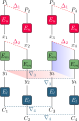
\includegraphics[width=0.55\textwidth]{./figures/sandwich.pdf}
\caption*{$P = \pr(P_3 \oplus P_4 = \Delta_1$)}
\end{figure}
\column[c]{0.5\textwidth}
\begin{figure}
\begin{center}
\begin{tikzpicture}[bc/.style={draw,minimum height=1cm, minimum width=.7cm, rounded corners=2pt}]
  \pgfmathsetmacro{\dx}{3};
  \pgfmathsetmacro{\dy}{1.6};
  \foreach \i/\labelside in {1/left, 2/right} {
    \draw (\dx*\i,0) node[below]     (P\i)  {$P_\i$}
          ++(0,-\dy) node[bc, fill=upper] (Eu\i) {\textcolor{white}{$E\Up$}}
          ++(0,-\dy) node[bc, fill=common] (Em\i) {$E\Mid$}
          ++(0,-\dy) node[bc, fill=lower] (El\i) {\textcolor{white}{$E\Low$}}
          ++(0,-\dy) node[above]    (C\i)  {$C_{\i}$};
    \draw[->] (P\i)  -- coordinate (Pp\i)           (Eu\i);
    \draw[->] (Eu\i) -- coordinate (Xp\i) node[\labelside] {$X_{\i}$} (Em\i);
    \draw[->] (Em\i) -- coordinate (Y\i) node[\labelside] {$Y_{\i}$} (El\i);
    \draw[->] (El\i) -- coordinate (Cc\i)           (C\i);
  }
  \draw[dashed, <->] (Pp1) -- node[tugred, above] (Pm) {$\Delta\In$} (Pp2);
  \draw[dashed, <->] (Xp1) -- node[tugred, above] (Xm) {\only<1>{$\Delta X$}} (Xp2);
  \draw[dashed, ->] (Pm)++(0, -\dy/4) -- node[right]{$p$} (Xm);
  \draw (Y1)++(0.5,0) node[mach] (Gm1) {\only<1>{$\Lambda Y$}}
        (Y2)++(-0.5,0) node[mach] (Gm2) {\only<1>{$\Lambda Y$}};
  \draw[dashed, ->] (Gm1) to[out=90, in=180] ($(Xm)+(0, -0.4)$) node[below] {$r$} to[out=0, in=90] (Gm2);
  \foreach \i/\labelside in {1/right, 2/left} {
    \draw (Gm\i|-C\i) node[mach] (Go\i) {$\lambda_o$};
    \draw[dashed, ->] (Gm\i) -- node[\labelside] {$q$} (Go\i);
    }
\end{tikzpicture}
\end{center}
\caption*{$\corr = \corr(\lambda_{o} \cdot (C_1 \oplus C_2))$}
\end{figure}
\end{columns}
\end{frame}

%%%%%%%%%%%%%%%%%%%%%%%%%%%%%%%%%%%%%%%%%%%%%%%%%%%%%%%%%%%%%%%%%%%%%%%%
\begin{frame}{Reuse the Tools from Boomerang Aanalysis in DL Analysis \cite{dlct_eurocrypt_BarOnDKW19, crypto_HDE2024}}
\begin{columns}
\column{0.5\textwidth}
\begin{table}[h!]
\centering
\begin{tabular}{c|c}
\textbf{Boomerang} & \textbf{Differential-Linear} \\
\toprule
\resizebox{0.3\textwidth}{!}{
\begin{tikzpicture}
  \pgfmathsetmacro{\lth}{1.5};
  \pgfmathsetmacro{\htt}{0.5};
  \node[tugred] (D1) at (0, 0) {$\Delta\In$};
  \node[right=\lth of D1, gray] (D2) {$\Delta\Out$};
  \node[below=\htt of D1, gray] (L1) {$\nabla\In$};
  \node[right=\lth of L1, blue] (L2) {$\nabla\Out$};
  \draw[->, gray] (D1) -- (D2);
  \draw[->] (D1) --node[above]{\bf\small\bct} (L2);
  \draw[<-, gray] (L1) -- (L2);
\end{tikzpicture}} &
\resizebox{0.3\textwidth}{!}{
\begin{tikzpicture}
  \pgfmathsetmacro{\lth}{1.5};
  \pgfmathsetmacro{\htt}{0.5};
  \node[tugred] (D1) at (0, 0) {$\Delta\In$};
  \node[right=\lth of D1, gray] (D2) {$\Delta\Out$};
  \node[below=\htt of D1, gray] (L1) {$\lambda\In$};
  \node[right=\lth of L1, blue] (L2) {$\lambda\Out$};
  \draw[->, gray] (D1) -- (D2);
  \draw[->] (D1) --node[above]{\bf\small\dlct} (L2);
  \draw[<-, gray] (L1) -- (L2);
\end{tikzpicture}} \\
\midrule
\resizebox{0.3\textwidth}{!}{
\begin{tikzpicture}
  \pgfmathsetmacro{\lth}{1.5};
  \pgfmathsetmacro{\htt}{0.5};
  \node[tugred] (D1) at (0, 0) {$\Delta\In$};
  \node[right=\lth of D1, tugred] (D2) {$\Delta\Out$};
  \node[below=\htt of D1, gray] (L1) {$\nabla\In$};
  \node[right=\lth of L1, blue] (L2) {$\nabla\Out$};
  \draw[->, gray] (D1) -- (D2);
  \draw[->] (D1) --node[above]{\bf\small\ubct} (L2);
  \draw[<-, gray] (L1) -- (L2);
\end{tikzpicture}} &
\resizebox{0.3\textwidth}{!}{
\begin{tikzpicture}
  \pgfmathsetmacro{\lth}{1.5};
  \pgfmathsetmacro{\htt}{0.5};
  \node[tugred] (D1) at (0, 0) {$\Delta\In$};
  \node[right=\lth of D1, tugred] (D2) {$\Delta\Out$};
  \node[below=\htt of D1, gray] (L1) {$\lambda\In$};
  \node[right=\lth of L1, blue] (L2) {$\lambda\Out$};
  \draw[->, gray] (D1) -- (D2);
  \draw[->] (D1) --node[above]{\bf\small\udlct} (L2);
  \draw[<-, gray] (L1) -- (L2);
\end{tikzpicture}} \\
\bottomrule
\end{tabular}
\end{table}

\column{0.5\textwidth}
\begin{table}[h!]
\centering
\begin{tabular}{c|c}
\textbf{Boomerang} & \textbf{Differential-Linear} \\
\toprule
\resizebox{0.3\textwidth}{!}{
\begin{tikzpicture}
  \pgfmathsetmacro{\lth}{1.5};
  \pgfmathsetmacro{\htt}{0.5};
  \node[tugred] (D1) at (0, 0) {$\Delta_1$};
  \node[right=\lth of D1, gray] (D2) {$\Delta_2$};
  \node[below=\htt of D1, blue] (L1) {$\nabla_1$};
  \node[right=\lth of L1, blue] (L2) {$\nabla_2$};
  \draw[->, gray] (D1) -- (D2);
  \draw[->] (D1) --node[above]{\bf\small\lbct} (L2);
  \draw[<-, gray] (L1) -- (L2);
\end{tikzpicture}} &
\resizebox{0.3\textwidth}{!}{
\begin{tikzpicture}
  \pgfmathsetmacro{\lth}{1.5};
  \pgfmathsetmacro{\htt}{0.5};
  \node[tugred] (D1) at (0, 0) {$\Delta\In$};
  \node[right=\lth of D1, gray] (D2) {$\Delta\Out$};
  \node[below=\htt of D1, blue] (L1) {$\lambda\In$};
  \node[right=\lth of L1, blue] (L2) {$\lambda\Out$};
  \draw[->, gray] (D1) -- (D2);
  \draw[->] (D1) --node[above]{\bf\small\ldlct} (L2);
  \draw[<-, gray] (L1) -- (L2);
\end{tikzpicture}} \\
\midrule
\resizebox{0.3\textwidth}{!}{
\begin{tikzpicture}
  \pgfmathsetmacro{\lth}{1.5};
  \pgfmathsetmacro{\htt}{0.5};
  \node[tugred] (D1) at (0, 0) {$\Delta_1$};
  \node[right=\lth of D1, tugred] (D2) {$\Delta_2$};
  \node[below=\htt of D1, blue] (L1) {$\nabla_1$};
  \node[right=\lth of L1, blue] (L2) {$\nabla_2$};
  \draw[->, gray] (D1) -- (D2);
  \draw[->] (D1) --node[above]{\bf\small\ebct} (L2);
  \draw[<-, gray] (L1) -- (L2);
\end{tikzpicture}} &
\resizebox{0.3\textwidth}{!}{
\begin{tikzpicture}
  \pgfmathsetmacro{\lth}{1.5};
  \pgfmathsetmacro{\htt}{0.5};
  \node[tugred] (D1) at (0, 0) {$\Delta\In$};
  \node[right=\lth of D1, tugred] (D2) {$\Delta\Out$};
  \node[below=\htt of D1, blue] (L1) {$\lambda\In$};
  \node[right=\lth of L1, blue] (L2) {$\lambda\Out$};
  \draw[->, gray] (D1) -- (D2);
  \draw[->] (D1) --node[above]{\bf\small\edlct} (L2);
  \draw[<-, gray] (L1) -- (L2);
\end{tikzpicture}} \\
\bottomrule
\end{tabular}
\end{table}
\end{columns}

\begin{table}
\centering
\begin{tabular}{c|c}
\textbf{Boomerang} & \textbf{Differential-Linear} \\
\toprule
\resizebox{0.4\textwidth}{!}{
  \begin{tikzpicture}
    \pgfmathsetmacro{\lth}{1.5};
    \pgfmathsetmacro{\htt}{0.5};
    \node[tugred] (D1) at (0, 0) {$\Delta\In$};
    \node[right=\lth of D1, gray] (D2) {$\Delta\Mid$};
    \node[right=\lth of D2, gray] (D3) {$\Delta\Out$};
    \node[below=\htt of D1, gray] (L1) {$\nabla\In$};
    \node[right=\lth of L1, gray] (L2) {$\nabla\Mid$};
    \node[right=\lth of L2, blue] (L3) {$\nabla\Out$};
    \draw[->] (D1) -- (D2);
    \draw[->, gray] (D2) -- (D3);
    \draw[->] (D1) -- (L2)node[above=0.3cm]{\dbct};
    \draw[->, gray] (L1) -- (L2);
    \draw[->, lower] (L2) -- (L3);
    \draw[->] (D2) -- (L3);
  \end{tikzpicture}} &
\resizebox{0.4\textwidth}{!}{
  \begin{tikzpicture}
    \pgfmathsetmacro{\lth}{1.5};
    \pgfmathsetmacro{\htt}{0.5};
    \node[tugred] (D1) at (0, 0) {$\Delta\In$};
    \node[right=\lth of D1, gray] (D2) {$\Delta\Mid$};
    \node[right=\lth of D2, gray] (D3) {$\Delta\Out$};
    \node[below=\htt of D1, gray] (L1) {$\lambda\In$};
    \node[right=\lth of L1, gray] (L2) {$\lambda\Mid$};
    \node[right=\lth of L2, blue] (L3) {$\lambda\Out$};
    \draw[->] (D1) -- (D2);
    \draw[->, gray] (D2) -- (D3);
    \draw[->] (D1) -- (L2)node[above=0.3cm]{\ddlct};
    \draw[->, gray] (L1) -- (L2);
    \draw[->, lower] (L2) -- (L3);
    \draw[->] (D2) -- (L3);
  \end{tikzpicture}} \\
\end{tabular}
\end{table}
\end{frame}

%%%%%%%%%%%%%%%%%%%%%%%%%%%%%%%%%%%%%%%%%%%%%%%%%%%%%%%%%%%%%%%%%%%%%%%%
\begin{frame}{Application of the Generalized \dlct Tables - AES ({\scriptsize\protect\dlfeistellegend})}
\vspace{-0.3cm}
\begin{figure}
%\resizebox{\textwidth}{!}{%
%\centering
%\input{aes_example.tex}
%}
  \colorlet{myred}{upper}
  \colorlet{myblue}{lower}
  \colorlet{mygray}{tuggray!50}
  \centering
  \begin{tikzpicture}[>=latex, 
                      stateopts/.style={scale=.35},
                      fillopts/.style={mach!50},
                      cellopts/.style={font=\scriptsize\color{white}}]
    \pgfmathsetmacro{\stepsep}{2} % between two cells with a labeled edge

    \draw[every node/.style={state}, rounded corners=2pt]
          (0,0)        node (S0) {\State{\Fill[myred]{ss32}\Cell{ss32}{\texttt{01}}}}
        ++(\stepsep,0) node (S1) {\State{\Fill[myred]{ss32}\Cell{ss32}{$\alpha$}}}
        ++(\stepsep,0) node (S2) {\State{\FillColumn[myred]{3}\Cell{ss03}{$\alpha$}\Cell{ss13}{$\alpha$}\Cell{ss23}{$3\alpha$}\Cell{ss33}{$2\alpha$}}}
        ++(\stepsep,0) node (S3) {\State{\FillColumn[mygray]{3}\Fill[myred]{ss03}\Cell{ss03}{$\beta$}}}
        ++(\stepsep,0) node (S4) {\State{\FillState[mygray]\FillColumn[myred]{3}\Cell{ss03}{$2\beta$}\Cell{ss13}{$3\beta$}\Cell{ss23}{$\beta$}\Cell{ss33}{$\beta$}}}
        ++(\stepsep,0) node (S5) {\State{\FillState[mygray]}}
        ;

    \foreach \in/\out/\label in {S0/S1/SB,S1/S2/{SR\\MC\\AK},
                                  S2/S3/SB,S3/S4/{SR\\MC\\AK},
                                  S4/S5/SB} {
    \draw[->] (\in) --node[above,align=center,font=\sffamily\tiny]{\label} (\out);
  }
  \foreach \st/\rr in {0/0, 2/1, 4/2} {
    \draw (S\st.north west) node[above right,font=\small] {R\rr};
  }
  \end{tikzpicture}
  \bigskip

  \begin{tikzpicture}[>=latex, 
                      stateopts/.style={scale=.35},
                      fillopts/.style={mach!50},
                      cellopts/.style={font=\scriptsize\color{white}}]
    \pgfmathsetmacro{\stepsep}{2} % between two cells with a labeled edge

    \draw[every node/.style={state}, rounded corners=2pt]
          (0,0)        node (S0) {\State{\FillState[mygray]}}
        ++(\stepsep,0) node (S1) {\State{\FillState[mygray]\FillDiagonal[myblue]{3}\Cell{ss03}{$2\delta$}\Cell{ss10}{$3\delta$}\Cell{ss21}{$\delta$}\Cell{ss32}{$\delta$}}}
        ++(\stepsep,0) node (S2) {\State{\FillDiagonal[mygray]{3}\Fill[myblue]{ss03}\Cell{ss03}{$\delta$}}}
        ++(\stepsep,0) node (S3) {\State{\FillDiagonal[myblue]{3}\Cell{ss03}{$\gamma$}\Cell{ss10}{$\gamma$}\Cell{ss21}{$2\gamma$}\Cell{ss32}{$3\gamma$}}}
        ++(\stepsep,0) node (S4) {\State{\Fill[myblue]{ss23}\Cell{ss23}{$\gamma$}}}
        ++(\stepsep,0) node (S5) {\State{\Fill[myblue]{ss23}\Cell{ss23}{\texttt{09}}}}
        ;

    \foreach \in/\out/\label in {S0/S1/SB,S1/S2/{SR\\MC\\AK},
                                  S2/S3/SB,S3/S4/{SR\\MC\\AK},
                                  S4/S5/SB} {
    \draw[->] (\in) --node[above,align=center,font=\sffamily\tiny]{\label} (\out);
  }
  \foreach \st/\rr in {0/0, 2/1, 4/2} {
    \draw (S\st.south west) node[below right,font=\small] {R\rr};
  }
  \end{tikzpicture}
\end{figure}
\[\sum_{\alpha, \beta, \gamma, \delta} \mathbb{C}_{\udlct}({\tt 1},\alpha,\delta) \cdot \mathbb{C}_{\edlct}(\alpha,\beta,\delta,\gamma)\cdot \mathbb{C}_{\ldlct}(\beta,\gamma,{\tt 9}) = -2^{-7.94}\]
\end{frame}

%%%%%%%%%%%%%%%%%%%%%%%%%%%%%%%%%%%%%%%%%%%%%%%%%%%%%%%%%%%%%%%%%%%%%%%%
\begin{frame}{Overview of Our Method to Search for Distinguishers in Sandwich Framework}
\begin{figure}
  \begin{tikzpicture}[yscale=1,xscale=1,baseline=0, decoration={
    markings,
    mark=at position 0.5 with {\arrow{>>}}}]
  \pgfmathsetmacro{\hstep}{3.5}
  \pgfmathsetmacro{\vstep}{1.2}
  \pgfmathsetmacro{\halfvstep}{\vstep/2}
  \pgfmathsetmacro{\quartervstep}{\vstep/4}
  \pgfmathsetmacro{\halfhstep}{\hstep/2}
  \pgfmathsetmacro{\quarterhstep}{\hstep/4}
  
  \visible<1>{
  \node (c1) at (0, 0) {};
  \node[right=\hstep of c1] (c2) {};
  \node[right=\hstep of c2] (c3) {};
  \node[right=\hstep of c3] (c4) {};
  \draw[rounded corners=2pt] ($(c1) + (0, -\halfvstep)$) rectangle ($(c4) + (0, \halfvstep)$) node[pos=0.5] {\only<1>{$E$}\only<2->{$E_{m}$}};
	\draw[<->, dashed, white] ($(c1) + (0, \halfvstep + 0.1)$) -- node[above] {$r_{0}$} ($(c2) + (0,\halfvstep + 0.1)$);
  }

  \visible<2-5>{
  \draw[rounded corners=2pt] ($(c1) + (0, -\halfvstep)$) rectangle ($(c4) + (0, \halfvstep)$) node[pos=0.5] {$E\Mid$};
  \draw[] ($(c2) + (0, -\halfvstep)$) -- ($(c2) + (0, \halfvstep + 0.2)$);
  \draw[] ($(c3) + (0, -\halfvstep)$) -- ($(c3) + (0, \halfvstep + 0.2)$);
  \draw[<->, dashed] ($(c1) + (0, \halfvstep + 0.1)$) -- node[above] {$r\Up$} ($(c2) + (0,\halfvstep + 0.1)$);
  \draw[<->, dashed] ($(c2) + (0, \halfvstep + 0.1)$) -- node[above] {$r\Mid$} ($(c3) + (0,\halfvstep + 0.1)$);
  \draw[<->, dashed] ($(c3) + (0, \halfvstep + 0.1)$) -- node[above] {$r\Low$} ($(c4) + (0,\halfvstep + 0.1)$);
  \node[] (e0) at ($0.5*(c1) + 0.5*(c2)$) {$E\Up$};
  \node[] (e1) at ($0.5*(c3) + 0.5*(c4)$) {$E\Low$};
  }

  \only<3-5>{
    \draw[fill=upper, opacity=0.6] ($(c1) + (0, 1.2*\quartervstep)$) -- ($(c2) + (0, 0.3*\quartervstep)$) -- ($(c2) + (0, -0.3*\quartervstep)$) -- ($(c1) + (0, -1.2*\quartervstep)$) -- cycle;
    \draw[fill=upper, opacity=0.6] ($(c2) + (0, 0.3*\quartervstep)$) -- ($(c3) + (0, 1.6*\quartervstep)$) -- ($(c3) + (0, -1.6*\quartervstep)$) -- ($(c2) + (0, -0.3*\quartervstep)$) -- cycle;
  }
  \only<4-5>{
    \draw[fill=lower, opacity=0.6] ($(c2) + (0, 1.6*\quartervstep)$) -- ($(c3) + (0, 0.3*\quartervstep)$) -- ($(c3) + (0, -0.3*\quartervstep)$) -- ($(c2) + (0, -1.6*\quartervstep)$) -- cycle;
    \draw[fill=lower, opacity=0.6] ($(c3) + (0, 0.3*\quartervstep)$) -- ($(c4) + (0, 1.2*\quartervstep)$) -- ($(c4) + (0, -1.2*\quartervstep)$) -- ($(c3) + (0, -0.3*\quartervstep)$) -- cycle;
  }

  \visible<3-5>{
  \node[below=\vstep+0.2 of c1] (c1) {};
  \node[right=\hstep of c1] (c2) {};
  \node[right=\hstep of c2] (c3) {};
  \node[right=\hstep of c3] (c4) {};
  \coordinate[left=0.4 of c1] (di);
  \draw[->] (di) --node[above]{$\Delta\In$} (di-|c1);
  \coordinate[right=0.4 of c3] (lm);
  \draw[->] (lm) --node[above]{$\lambda\Mid$} (lm-|c3);
  \draw[] ($(c2) + (0, -\halfvstep)$) -- ($(c2) + (0, \halfvstep)$);
  \draw[rounded corners=2pt] ($(c1) + (0, -\halfvstep)$) rectangle ($(c3) + (0, \halfvstep)$);
  
  \visible<3-4>{
  \node[box, minimum size=9, fill=upper] at ($(c1) + (\quarterhstep, \quartervstep)$) {{\scriptsize $s$}};
  \node[box, minimum size=9] at ($(c1) + (\quarterhstep, 0)$) {{\scriptsize $s$}};
  \node[box, minimum size=9, fill=upper] at ($(c1) + (\quarterhstep, -\quartervstep)$) {{\scriptsize $s$}};
  
  \node[box, minimum size=9, fill=upper] at ($(c1.east) + (\halfhstep, \quartervstep)$) {{\scriptsize $s$}};
  \node[box, minimum size=9] at ($(c1.east) + (\halfhstep, 0)$) {{\scriptsize $s$}};
  \node[box, minimum size=9, fill=upper] at ($(c1.east) + (\halfhstep, -\quartervstep)$) {{\scriptsize $s$}};
  
  \node[box, minimum size=9] at ($(c2) + (-\quarterhstep, \quartervstep)$) {{\scriptsize $s$}};
  \node[box, minimum size=9, fill=upper] at ($(c2) + (-\quarterhstep, 0)$) {{\scriptsize $s$}};
  \node[box, minimum size=9] at ($(c2) + (-\quarterhstep, -\quartervstep)$) {{\scriptsize $s$}};
  
  \node[box, minimum size=9] at ($(c2) + (\quarterhstep, \quartervstep)$) {{\scriptsize $s$}};
  \node[box, minimum size=9, fill=common] at ($(c2) + (\quarterhstep, 0)$) {{\scriptsize $s$}};
  \node[box, minimum size=9] at ($(c2) + (\quarterhstep, -\quartervstep)$) {{\scriptsize $s$}};
  
  \node[box, minimum size=9] at ($(c2.east) + (\halfhstep, \quartervstep)$) {{\scriptsize $s$}};
  \node[box, minimum size=9, fill=common] at ($(c2.east) + (\halfhstep, 0)$) {{\scriptsize $s$}};
  \node[box, minimum size=9, fill=upper] at ($(c2.east) + (\halfhstep, -\quartervstep)$) {{\scriptsize $s$}};
  
  \node[box, minimum size=9, fill=upper] at ($(c3) + (-\halfhstep + \quarterhstep, \quartervstep)$) {{\scriptsize $s$}};
  \node[box, minimum size=9, fill=upper] at ($(c3) + (-\halfhstep + \quarterhstep, 0)$) {{\scriptsize $s$}};
  \node[box, minimum size=9, fill=common] at ($(c3) + (-\halfhstep + \quarterhstep, -\quartervstep)$) {{\scriptsize $s$}};
  }
  \draw[|-|, postaction={decorate}, thick] ($(c1) + (0, \halfvstep + 0.2)$) -- ($(c2) + (0,\halfvstep + 0.2)$);
  \draw[-|, postaction={decorate}, thick, dashed] ($(c2) + (0, \halfvstep + 0.2)$) -- ($(c3) + (0,\halfvstep + 0.2)$);
  }

  \visible<5>{
    \node[] at ($0.5*(c1) + 0.5*(c2)$) (temp) {\small \textcolor{tugred}{$\tilde{u}_{0}, \ldots, \tilde{u}_{k - 1}$}};
    \node[] at ($0.5*(c2) + 0.5*(c3)$) (temp) {\small \textcolor{tugred}{$u_{0}, \ldots, u_{t - 1}$}};
  }
  \visible<4-5>{
  \node[below=\vstep of c1] (c1) {};
  \node[right=\hstep of c1] (c2) {};
  \node[right=\hstep of c2] (c3) {};
  \node[right=\hstep of c3] (c4) {};
  \coordinate[left=0.5 of c2] (dm);
  \draw[->] (dm) --node[above]{$\Delta\Mid$} (dm-|c2);
  \coordinate[right=0.4 of c4] (lo);
  \draw[->] (lo) --node[above]{$\lambda\Out$} (lo-|c4);
  \draw[] ($(c3) + (0, -\halfvstep)$) -- ($(c3) + (0, \halfvstep)$);
  \draw[rounded corners=2pt] ($(c2) + (0, -\halfvstep)$) rectangle ($(c4) + (0, \halfvstep)$);
  
  \visible<4>{
  \node[box, minimum size=9, fill=lower] at ($(c2) + (\quarterhstep, \quartervstep)$) {{\scriptsize $s$}};
  \node[box, minimum size=9, fill=common] at ($(c2) + (\quarterhstep, 0)$) {{\scriptsize $s$}};
  \node[box, minimum size=9, fill=lower] at ($(c2) + (\quarterhstep, -\quartervstep)$) {{\scriptsize $s$}};
  
  \node[box, minimum size=9, fill=lower] at ($(c2.east) + (\halfhstep, \quartervstep)$) {{\scriptsize $s$}};
  \node[box, minimum size=9, fill=common] at ($(c2.east) + (\halfhstep, 0)$) {{\scriptsize $s$}};
  \node[box, minimum size=9] at ($(c2.east) + (\halfhstep, -\quartervstep)$) {{\scriptsize $s$}};
  
  \node[box, minimum size=9] at ($(c3) + (-\quarterhstep, +\quartervstep)$) {{\scriptsize $s$}};
  \node[box, minimum size=9] at ($(c3) + (-\quarterhstep, 0)$) {{\scriptsize $s$}};
  \node[box, minimum size=9, fill=common] at ($(c3) + (-\halfhstep + \quarterhstep, -\quartervstep)$) {{\scriptsize $s$}};
  
  \node[box, minimum size=9] at ($(c3) + (\quarterhstep, \quartervstep)$) {{\scriptsize $s$}};
  \node[box, minimum size=9] at ($(c3) + (\quarterhstep, 0)$) {{\scriptsize $s$}};
  \node[box, minimum size=9, fill=lower] at ($(c3) + (\quarterhstep, -\quartervstep)$) {{\scriptsize $s$}};
  
  \node[box, minimum size=9, fill=lower] at ($(c3.east) + (\halfhstep, \quartervstep)$) {{\scriptsize $s$}};
  \node[box, minimum size=9] at ($(c3.east) + (\halfhstep, 0)$) {{\scriptsize $s$}};
  \node[box, minimum size=9, fill=lower] at ($(c3.east) + (\halfhstep, -\quartervstep)$) {{\scriptsize $s$}};
  
  \node[box, minimum size=9, fill=lower] at ($(c4) + (-\quarterhstep, +\quartervstep)$) {{\scriptsize $s$}};
  \node[box, minimum size=9] at ($(c4) + (-\quarterhstep, 0)$) {{\scriptsize $s$}};
  \node[box, minimum size=9, fill=lower] at ($(c4) + (-\quarterhstep, -\quartervstep)$) {{\scriptsize $s$}};
  }
  \draw[|-|, postaction={decorate}, thick, dashed] ($(c3) - (0, \halfvstep + 0.2)$) -- ($(c2) - (0,\halfvstep + 0.2)$);
  \draw[|-, postaction={decorate}, thick] ($(c4) - (0, \halfvstep + 0.2)$) -- ($(c3) - (0,\halfvstep + 0.2)$);
  }
  \visible<5>{
    \draw[rounded corners=2pt] ($(c2) + (0, -\halfvstep)$) rectangle ($(c4) + (0, \halfvstep)$);
    \node[] at ($0.5*(c2) + 0.5*(c3)$) (temp) {\small \textcolor{mach}{$\ell_{0}, \ldots, \ell_{t - 1}$}};
    \node[] at ($(c1.east) + (\halfhstep, +\halfvstep + 0.15)$) (w0) {\scriptsize $w\Up$};
    \draw[<-, dashed] ($(c1) + (0, +\halfvstep + 0.15)$) -- (w0);
    \draw[->, dashed] (w0) -- ($(c2) + (0, +\halfvstep + 0.15)$);
    \node[] at ($(c2.east) + (\halfhstep, +\halfvstep + 0.15)$) (wm) {\scriptsize $w\Mid$};
    \draw[<-, dashed] ($(c2) + (0, +\halfvstep + 0.15)$) -- (wm);
    \draw[->, dashed] (wm) -- ($(c3) + (0, +\halfvstep + 0.15)$);
    \node[] at ($0.5*(c3) + 0.5*(c4)$) (temp) {\small \textcolor{mach}{$\tilde{\ell}_{0}, \ldots, \tilde{\ell}_{n - 1}$}};
    \node[] at ($(c3.east) + (\halfhstep, +\halfvstep + 0.15)$) (w1) {\scriptsize $w\Low$};
    \draw[<-, dashed] ($(c3) + (0, +\halfvstep + 0.15)$) -- (w1);
    \draw[->, dashed] (w1) -- ($(c4) + (0, +\halfvstep + 0.15)$);
    \node[] at ($0.5*(c2) + 0.5*(c3) + (0, -1.1*\vstep-\quartervstep)$) {\small $\min \left(\sum_{i = 0}^{k - 1} \textcolor{tugred}{w\Up}\cdot \textcolor{tugred}{\tilde{u}_{i}} + \sum_{j = 0}^{t - 1} \textcolor{black}{w\Mid}\cdot \textcolor{black}{\booltoint\left(\textcolor{tugred}{\ell_{j}} + \textcolor{mach}{u_{j}} = 2\right)} + \sum_{k = 0}^{n - 1} \textcolor{mach}{w\Low}\cdot \textcolor{mach}{\tilde{\ell}_{k}}\right)$};
  }
  \end{tikzpicture}
  \smallskip\par
  \tikzset{rounded corners=2pt}
  \visible<3-4>{
  \legendwrap{\Fill[upper]{0,0}} differentially active S-box\quad
  \legendwrap{\Fill[lower]{0,0}} linearly active S-box\quad
  \legendwrap{\Fill[common]{0,0}} common active S-box
  }
\end{figure}
\end{frame}

%%%%%%%%%%%%%%%%%%%%%%%%%%%%%%%%%%%%%%%%%%%%%%%%%%%%%%%%%%%%%%%%%%%%%%%%
\begin{frame}{Example: A 5-round DL Distinguisher for \cipher{AES}}
\begin{center}
\includegraphics[width=\textwidth]{./figures/aes_sk_5r_v0.pdf} % Replace with your third shape
\end{center}
\begin{center}
  \resizebox{0.9\textwidth}{!}{
\begin{tabular}{@{}cc@{}}
  \toprule
  \multicolumn{2}{c}{$r_{0} = 1, r_{m} = 3, r_{1} = 1, ~ p = 2^{-24.00}, r = 2^{-7.66}, ~ q^{2} = 2^{-24.00}, ~ prq^{2} = 2^{-55.66}$}\\
  \midrule
  $\Delta X_{0}$ \small\texttt{001c00000000e200000000dfb3000000} & $\Delta X_{1}$ \small\texttt{000000000000000000f7000000000000}\\
  $\Gamma X_{4}$ \small\texttt{00000000000000006700000000000000} & $\Gamma X_{5}$ \small\texttt{21d3814d93b1ef228e923507f67383fd}\\
  \bottomrule
\end{tabular}}
\end{center}
\end{frame}


%%%%%%%%%%%%%%%%%%%%%%%%%%%%%%%%%%%%%%%%%%%%%%%%%%%%%%%%%%%%%%%%%%%%%%%%
\begin{frame}{Example: Distinguishers for up to 8 Rounds of \cipher{CLEFIA} \cite{crypto_HDE2024}}
\begin{itemize}
  \item Comparing the data complexity of best boomerang and DL distinguishers
\end{itemize}
\begin{center}
\begin{tabular}[t]{c|c|c|c}
\toprule
\# Rounds    &  Boomerang \cite{tosc_HadipourNE22} & Differential-Linear \cite{crypto_HDE2024}& Gain\\
\midrule
3            &  1            & 1           & 1\\
4            &  $2^{6.32}$   & 1           & $2^{6.32}$\\
5            &  $2^{12.26}$  & $2^{5.36}$  & $2^{6.90}$\\
6            &  $2^{22.45}$  & $2^{14.14}$ & $2^{8.31}$\\
7            &  $2^{32.67}$  & $2^{23.50}$ & $2^{9.17}$\\
8            &  $2^{76.03}$  & $2^{66.86}$ & $2^{9.17}$\\
\bottomrule
\end{tabular}
\end{center}
\end{frame}

%%%%%%%%%%%%%%%%%%%%%%%%%%%%%%%%%%%%%%%%%%%%%%%%%%%%%%%%%%%%%%%%%%%%%%%%
\section{Research Gaps and Future Works}

%%%%%%%%%%%%%%%%%%%%%%%%%%%%%%%%%%%%%%%%%%%%%%%%%%%%%%%%%%%%%%%%%%%%%%%%
\begin{frame}{Lessons and Future Works}
\begin{itemize}
  \large
  \item Lessons learned:
  \begin{itemize}
    \item[\color{tugred}{\faDiamond}] Consider the theoretical links between attacks in automated discovery.  
    \item[\color{tugred}{\faDiamond}] Consider the structural similarities between attacks in automated discovery. 
  \end{itemize}
  \item \textbf{Future works}:
  \begin{itemize}
    \item[\color{tugblue}{\faRoad}] Connections between attacks are underutilized in automated discovery.
    \item[\color{tugblue}{\faRoad}] Existing methods often lack either accuracy or efficiency (hard to achieve both).
    \item[\color{tugblue}{\faRoad}] No unified framework exists for finding complete attacks across various types, e.g., differential, linear, boomerang.
    \item[\color{tugblue}{\faRoad}] Current methods are limited to strongly aligned designs, lacking approaches for weakly aligned designs.
  \end{itemize}
\end{itemize}
\end{frame}

% ######################################################################
\begin{frame}{A Sentence from My Mom That is Relevant to Cryptanalysis}
\begin{center}
\textit{\textbf{\Huge "In this world, there is a universal law: to gain something, you must lose something else."}}\\
\vspace{0.5cm}
\textit{\textbf{\Huge -- My Mom}}
\end{center}
\begin{center}
\Large
\vspace{1cm}
\faGithub: \url{https://github.com/hadipourh/talks}
\end{center}
\end{frame}

% ######################################################################
% ######################################################################
% ######################################################################
% Bakcup slides

\include{backupslides}
% ######################################################################
% ######################################################################
% ######################################################################

\begin{filecontents*}[overwrite]{\jobname.bib}

% Seminal paper of Differential-Linear Cryptanalysis
@inproceedings{dl_crypto_LangfordH94,
  author       = {Susan K. Langford and
                  Martin E. Hellman},
  title        = {Differential-Linear Cryptanalysis},
  booktitle    = {{CRYPTO} '94},
  volume       = {839},
  pages        = {17--25},
  publisher    = {Springer},
  year         = {1994},
  doi          = {10.1007/3-540-48658-5_3}
}

% AES specification
@article{daemen1999aes,
  title={AES proposal: Rijndael},
  author={Daemen, Joan and Rijmen, Vincent},
  year={1999},
  publisher={Gaithersburg, MD, USA}
}

% seminal paper for differential cryptanalysis
@inproceedings{crypto_BihamS90,
  author       = {Eli Biham and
                  Adi Shamir},
  editor       = {Alfred Menezes and
                  Scott A. Vanstone},
  title        = {Differential Cryptanalysis of {DES}-like Cryptosystems},
  booktitle    = {{CRYPTO} '90},
  series       = {LNCS},
  volume       = {537},
  pages        = {2--21},
  publisher    = {Springer},
  year         = {1990},
  doi          = {10.1007/3-540-38424-3_1}
}

% seminal paper for linear cryptanalysis (Piling-up lemma)
@inproceedings{eurocrypt_Matsui93,
  author       = {Mitsuru Matsui},
  editor       = {Tor Helleseth},
  title        = {Linear Cryptanalysis Method for {DES} Cipher},
  booktitle    = {{EUROCRYPT} '93},
  series       = {LNCS},
  volume       = {765},
  pages        = {386--397},
  publisher    = {Springer},
  year         = {1993},
  doi          = {10.1007/3-540-48285-7_33}
}

% Formalizes the complexity of DL attacks
@article{journals_joc_BlondeauLN17,
  author       = {C{\'{e}}line Blondeau and
                  Gregor Leander and
                  Kaisa Nyberg},
  title        = {Differential-Linear Cryptanalysis Revisited},
  journal      = {J. Cryptol.},
  volume       = {30},
  number       = {3},
  pages        = {859--888},
  year         = {2017},
  doi          = {10.1007/s00145-016-9237-5}
}

% sandwich framework
@article{joc_DunkelmanKS14,
  author       = {Orr Dunkelman and
                  Nathan Keller and
                  Adi Shamir},
  title        = {A Practical-Time Related-Key Attack on the {KASUMI} Cryptosystem Used
                  in {GSM} and {3G} Telephony},
  journal      = {J. Cryptol.},
  volume       = {27},
  number       = {4},
  pages        = {824--849},
  year         = {2014},
  doi          = {10.1007/s00145-013-9154-9}
}

% DLCT paper. This is also the first paper splitting the cipher into three parts for DL analysis.
@inproceedings{dlct_eurocrypt_BarOnDKW19,
  author       = {Achiya Bar{-}On and
                  Orr Dunkelman and
                  Nathan Keller and
                  Ariel Weizman},
  title        = {{DLCT:} {A} New Tool for Differential-Linear Cryptanalysis},
  booktitle    = {{EUROCRYPT} 2019},
  series       = {LNCS},
  volume       = {11476},
  pages        = {313--342},
  publisher    = {Springer},
  year         = {2019},
  doi          = {10.1007/978-3-030-17653-2_11}
}

@inproceedings{fse_Wagner99,
  author    = {David A. Wagner},
  title     = {The Boomerang Attack},
  booktitle = {{FSE}},
  series    = {LNCS},
  volume    = {1636},
  pages     = {156--170},
  publisher = {Springer},
  doi       = {10.1007/3-540-48519-8_12},
  year      = {1999}
}

@inproceedings{fse_BlondeauLN14,
  author       = {C{\'{e}}line Blondeau and
                  Gregor Leander and
                  Kaisa Nyberg},
  editor       = {Carlos Cid and
                  Christian Rechberger},
  title        = {Differential-Linear Cryptanalysis Revisited},
  booktitle    = {{FSE} 2014},
  series       = {LNCS},
  volume       = {8540},
  pages        = {411--430},
  publisher    = {Springer},
  year         = {2014},
  doi          = {10.1007/978-3-662-46706-0_21},
}

@inproceedings{conf_crypto_DunkelmanKS10,
	author    = {Orr Dunkelman and
		         Nathan Keller and
		         Adi Shamir},
	title     = {A Practical-Time Related-Key Attack on the {KASUMI} Cryptosystem Used
		in {GSM} and 3G Telephony},
	booktitle = {{CRYPTO}},
	series    = {LNCS},
	volume    = {6223},
	pages     = {393--410},
	publisher = {Springer},
	doi       = {10.1007/978-3-642-14623-7_21},
	year      = {2010}
}

@inproceedings{eurocrypt_CidHPSS18,
  author       = {Carlos Cid and
                  Tao Huang and
                  Thomas Peyrin and
                  Yu Sasaki and
                  Ling Song},
  editor       = {Jesper Buus Nielsen and
                  Vincent Rijmen},
  title        = {Boomerang Connectivity Table: {A} New Cryptanalysis Tool},
  booktitle    = {{EUROCRYPT} 2018},
  series       = {LNCS},
  volume       = {10821},
  pages        = {683--714},
  publisher    = {Springer},
  year         = {2018},
  doi          = {10.1007/978-3-319-78375-8_22}
}

@article{tosc_WangP19,
  author       = {Haoyang Wang and
                  Thomas Peyrin},
  title        = {Boomerang Switch in Multiple Rounds. Application to {AES} Variants
                  and Deoxys},
  journal      = {{IACR} Trans. Symmetric Cryptol.},
  volume       = {2019},
  number       = {1},
  pages        = {142--169},
  year         = {2019},
  doi          = {10.13154/TOSC.V2019.I1.142-169}
}

@article{tosc_DelauneDV20,
  author       = {St{\'{e}}phanie Delaune and
                  Patrick Derbez and
                  Mathieu Vavrille},
  title        = {Catching the Fastest Boomerangs Application to {SKINNY}},
  journal      = {{IACR} Trans. Symmetric Cryptol.},
  volume       = {2020},
  number       = {4},
  pages        = {104--129},
  year         = {2020},
  doi          = {10.46586/TOSC.V2020.I4.104-129}
}

@article{tosc_SongQH19,
  author       = {Ling Song and
                  Xianrui Qin and
                  Lei Hu},
  title        = {Boomerang Connectivity Table Revisited. Application to {SKINNY} and
                  {AES}},
  journal      = {{IACR} Trans. Symmetric Cryptol.},
  volume       = {2019},
  number       = {1},
  pages        = {118--141},
  year         = {2019},
  url          = {https://doi.org/10.13154/tosc.v2019.i1.118-141},
  doi          = {10.13154/TOSC.V2019.I1.118-141},
}

@article{tosc_BoukerrouHLMM20,
  author       = {Hamid Boukerrou and
                  Paul Huynh and
                  Virginie Lallemand and
                  Bimal Mandal and
                  Marine Minier},
  title        = {On the Feistel Counterpart of the Boomerang Connectivity Table Introduction
                  and Analysis of the {FBCT}},
  journal      = {{IACR} Trans. Symmetric Cryptol.},
  volume       = {2020},
  number       = {1},
  pages        = {331--362},
  year         = {2020},
  doi          = {10.13154/TOSC.V2020.I1.331-362},
}

@article{tosc_HadipourBS21,
  author       = {Hosein Hadipour and
                  Nasour Bagheri},
  title        = {Improved Rectangle Attacks on {SKINNY} and {CRAFT}},
  journal      = {{IACR} Trans. Symmetric Cryptol.},
  volume       = {2021},
  number       = {2},
  pages        = {140--198},
  year         = {2021},
  doi          = {10.46586/TOSC.V2021.I2.140-198},
}

% more precise measurement of bias for 9-round DL distinguisher of serpent
@inproceedings{indocrypt_DunkelmanIK08,
  author       = {Orr Dunkelman and
                  Sebastiaan Indesteege and
                  Nathan Keller},
  editor       = {Dipanwita Roy Chowdhury and
                  Vincent Rijmen and
                  Abhijit Das},
  title        = {A Differential-Linear Attack on 12-Round {Serpent}},
  booktitle    = {{INDOCRYPT} 2008},
  series       = {LNCS},
  volume       = {5365},
  pages        = {308--321},
  publisher    = {Springer},
  year         = {2008},
  doi          = {10.1007/978-3-540-89754-5_24}
}

% application of miqcp to simeck
@article{zhou2024milp,
  title        = {{MILP/MIQCP}-Based Fully Automatic Method of Searching for Differential-Linear Distinguishers for {SIMON}-Like Ciphers},
  author       = {Zhou, Yanyan and  
                  Wang, Senpeng and 
                  Hu, Bin},
  journal      = {IET Information Security},
  volume       = {2024},
  year         = {2024},
  publisher    = {Hindawi},
  doi          = {10.1049/2024/8315115}
}

% specification of CLEFIA
@inproceedings{conf_fse_ShiraiSAMI07,
  author    = {Taizo Shirai and
               Kyoji Shibutani and
               Toru Akishita and
               Shiho Moriai and
               Tetsu Iwata},
  title     = {The 128-Bit Blockcipher {CLEFIA} (Extended Abstract)},
  booktitle = {{FSE} 2007},
  series    = {LNCS},
  volume    = {4593},
  pages     = {181--195},
  publisher = {Springer},
  year      = {2007}
}

% skinny specification
@inproceedings{skinny_spec,  
  author    = {Beierle, Christof and 
              Jean, J{\'e}r{\'e}my and 
              K{\"o}lbl, Stefan and 
              Leander, Gregor and 
              Moradi, Amir and 
              Peyrin, Thomas and 
              Sasaki, Yu and 
              Sasdrich, Pascal and 
              Sim, Siang Meng},
  title     = {{The SKINNY family of block ciphers and its low-latency variant MANTIS}},
  Xbooktitle= {Advances in Cryptology -- CRYPTO 2016},
  booktitle = {{CRYPTO} 2016},
  pages     = {123--153},
  year      = {2016},
  organization= {Springer},
  doi       = {10.1007/978-3-662-53008-5_5},
}

% specification of TRIVIUM
@incollection{canniere2008trivium,
  title     = {Trivium},
  author    = {Canni{\`e}re, Christophe De and Preneel, Bart},
  booktitle = {New stream cipher designs},
  pages     = {244--266},
  year      = {2008},
  publisher = {Springer}
}

% specification of ZUC
@article{zuc128_specification,
	author    = {ETSI/SAGE},
	title     = {Specification of the 3GPP confidentiality and integrity algorithms
	{128-EEA3} and {128-EIA3}: {ZUC} specification},
	journal   = {ETSI/SAGE, Document 2, Version 1.6},
	year      = {2011}
}

% Ascon (JoC)
@article{ascon_jocDobraunigEMS21,
  author    = {Christoph Dobraunig and
                Maria Eichlseder and
                Florian Mendel and
                Martin Schl{\"{a}}ffer},
  title     = {{Ascon} v1.2: Lightweight Authenticated Encryption and Hashing},
  journal   = {Journal of Cryptology},
  volume    = {34},
  number    = {3},
  pages     = {33},
  year      = {2021},
  doi       = {10.1007/s00145-021-09398-9},
}

% Ascon (Final NIST sumbission)
@misc{asconnist,
  author       = {Christoph Dobraunig and
                  Maria Eichlseder and
                  Florian Mendel and
                  Martin Schl{\"a}ffer},
  howpublished = {Finalist submission to the NIST lightweight cryptography standardization process},
  title        = {{{Ascon} v1.2 (Submission to NIST)}},
  year         = {2021},
  url          = {https://csrc.nist.gov/Projects/Lightweight-Cryptography}
}

% specification of Keccak
@inproceedings{eurocrypt_BertoniDPA13,
  author    = {Guido Bertoni and
               Joan Daemen and
               Micha{\"{e}}l Peeters and
               Gilles Van Assche},
  title     = {Keccak},
  booktitle = {{EUROCRYPT}},
  series    = {Lecture Notes in Computer Science},
  volume    = {7881},
  pages     = {313--314},
  publisher = {Springer},
  year      = {2013},
  doi       = {10.1007/978-3-642-38348-9_19}
}

% specification of Enocoro-128v2
@article{watanabe2010hardware,
  title     = {A Hardware-Oriented Light Weight Pseudo-Random Number Generator Enocoro-128v2. The 2010 Symposium on Cryptography and Information Security, SCIS 2010, 3D1-3},
  author    = {Watanabe, D and Okamoto, K and Kaneko, T},
  year      = {2010}
}

% QARMAv2 specification
@article{qarmav2_spec, 
  title        = {The {QARMAv2} Family of Tweakable Block Ciphers}, 
  author       = {Avanzi, Roberto and
                 Banik, Subhadeep and 
                 Dunkelman, Orr and 
                 Eichlseder, Maria and 
                 Ghosh, Shibam and 
                 Nageler, Marcel and 
                 Regazzoni, Francesco}, 
  volume       = {2023}, 
  number       = {3}, 
  journal      = {IACR Transactions on Symmetric Cryptology}, 
  year         = {2023}, 
  month        = {Sep.}, 
  pages        = {25-73},
  doi          = {10.46586/tosc.v2023.i3.25-73},   
}

% impossible differential Knudesen
@article{knudsen1998deal,
  title     = {DEAL-a 128-bit block cipher},
  author    = {Knudsen, Lars},
  journal   = {complexity},
  volume    = {258},
  number    = {2},
  pages     = {216},
  year      = {1998},
  publisher = {Citeseer}
}

% impossible differential Biham (miss-in-the-middle technique)
@inproceedings{eurocrypt_BihamBS99,
  author    = {Eli Biham and
               Alex Biryukov and
               Adi Shamir},
  title     = {Cryptanalysis of Skipjack Reduced to 31 Rounds Using Impossible Differentials},
  booktitle = {{EUROCRYPT} 1999},
  series    = {LNCS},
  volume    = {1592},
  pages     = {12--23},
  publisher = {Springer},
  year      = {1999},
  doi       = {10.1007/3-540-48910-X_2}
}

% integral attack as a theoretical generalization of differential cryptanalysis
@article{Lai1994,
author      =  {Lai, Xuejia},
Xeditor      = {Blahut, Richard E.
               and Costello, Daniel J.
              and Maurer, Ueli
              and Mittelholzer, Thomas},
title       = {Higher Order Derivatives and Differential Cryptanalysis},
booktitle   = {Communications and Cryptography: Two Sides of One Tapestry},
year        = {1994},
publisher   = {Springer US},
address     = {Boston, MA},
pages       = {227--233},
doi         = {10.1007/978-1-4615-2694-0_23},
}

% integral attack by Daemen
@inproceedings{square_fse_DaemenKR97,
  author    = {Joan Daemen and
               Lars R. Knudsen and
               Vincent Rijmen},
  title     = {The Block Cipher {Square}},
  booktitle = {{FSE} 1997},
  series    = {LNCS},
  volume    = {1267},
  pages     = {149--165},
  publisher = {Springer},
  year      = {1997},
  doi       = {10.1007/BFb0052343},
}

% seminal paper for cube attack
@inproceedings{eurocrypt_DinurS09,
  author       = {Itai Dinur and
                  Adi Shamir},
  editor       = {Antoine Joux},
  title        = {Cube Attacks on Tweakable Black Box Polynomials},
  booktitle    = {{EUROCRYPT} 2009},
  series       = {LNCS},
  volume       = {5479},
  pages        = {278--299},
  publisher    = {Springer},
  year         = {2009},
  doi          = {10.1007/978-3-642-01001-9_16},
}

% full-round differential attack on DES
@inproceedings{crypto_BihamS92,
  author       = {Eli Biham and
                  Adi Shamir},
  editor       = {Ernest F. Brickell},
  title        = {Differential Cryptanalysis of the Full 16-Round {DES}},
  booktitle    = {{CRYPTO} '92},
  series       = {LNCS},
  volume       = {740},
  pages        = {487--496},
  publisher    = {Springer},
  year         = {1992},
  doi          = {10.1007/3-540-48071-4_34},
}

% full-round related-key boomerang attack on AES-256
@inproceedings{crypto_BiryukovKN09,
  author       = {Alex Biryukov and
                  Dmitry Khovratovich and
                  Ivica Nikolic},
  editor       = {Shai Halevi},
  title        = {Distinguisher and Related-Key Attack on the Full {AES-256}},
  booktitle    = {{CRYPTO} 2009},
  series       = {LNCS},
  volume       = {5677},
  pages        = {231--249},
  publisher    = {Springer},
  year         = {2009},
  doi          = {10.1007/978-3-642-03356-8_14},
}

% Enhanced DL (Using a non-deterministic differential trail in DL for the first time)
@inproceedings{enhanced_dl_asiacrypt_BihamDK02,
  author       = {Eli Biham and
                  Orr Dunkelman and
                  Nathan Keller},
  title        = {Enhancing Differential-Linear Cryptanalysis},
  booktitle    = {{ASIACRYPT} 2002},
  series       = {LNCS},
  volume       = {2501},
  pages        = {254--266},
  publisher    = {Springer},
  year         = {2002},
  doi          = {10.1007/3-540-36178-2_16},
}

% full-round integral attack on MISTY1
@inproceedings{crypto_Todo15,
  author       = {Yosuke Todo},
  editor       = {Rosario Gennaro and
                  Matthew Robshaw},
  title        = {Integral Cryptanalysis on Full {MISTY1}},
  booktitle    = {{CRYPTO} 2015},
  series       = {LNCS},
  volume       = {9215},
  pages        = {413--432},
  publisher    = {Springer},
  year         = {2015},
  doi          = {10.1007/978-3-662-47989-6_20},
}

% first cube attack on SHA3
@inproceedings{eurocrypt_HuangWXWZ17,
  author       = {Senyang Huang and
                  Xiaoyun Wang and
                  Guangwu Xu and
                  Meiqin Wang and
                  Jingyuan Zhao},
  editor       = {Jean{-}S{\'{e}}bastien Coron and
                  Jesper Buus Nielsen},
  title        = {Conditional Cube Attack on Reduced-Round Keccak Sponge Function},
  booktitle    = {{EUROCRYPT} 2017},
  series       = {LNCS},
  volume       = {10211},
  pages        = {259--288},
  year         = {2017},
  doi          = {10.1007/978-3-319-56614-6\_9},
}

@inproceedings{mine_acns_HadipourE22,
  author       = {\textbf{Hosein Hadipour} and
                  Maria Eichlseder},
  editor       = {Giuseppe Ateniese and
                  Daniele Venturi},
  title        = {Autoguess: {A} Tool for Finding Guess-and-Determine Attacks and Key
                  Bridges},
  booktitle    = {{\textbf{ACNS}} 2022},
  series       = {LNCS},
  volume       = {13269},
  pages        = {230--250},
  publisher    = {Springer},
  year         = {2022},
  doi          = {10.1007/978-3-031-09234-3_12},
  keywords     = {mypaper}
}

% automatic bit-wise search for ZC/Integral distinguishers
@article{tosc_HadipourSNSB19,
  author    = {\textbf{Hosein Hadipour} and
               Sadegh Sadeghi and
               Majid M. Niknam and
               Ling Song and
               Nasour Bagheri},
  title     = {Comprehensive security analysis of {CRAFT}},
  journal   = {{IACR} Trans. Symmetric Cryptol.},
  volume    = {2019},
  number    = {4},
  pages     = {290--317},
  year      = {2019},
  doi       = {10.13154/tosc.v2019.i4.290-317},
  keywords  = {mypaper}
}

% monomial_prediction_warp
@article{tosc_HadipourE22,
  author    = {\textbf{Hosein Hadipour} and
               Maria Eichlseder},
  title     = {Integral Cryptanalysis of {WARP} based on Monomial Prediction},
  journal   = {{IACR} Trans. Symmetric Cryptol.},
  volume    = {2022},
  number    = {2},
  pages     = {92--112},
  year      = {2022},
  doi       = {10.46586/tosc.v2022.i2.92-112},
  keywords  = {mypaper}
}

@inproceedings{eurocrypt_HadipourSE23,
  author       = {\textbf{Hosein Hadipour} and
                  Sadegh Sadeghi and
                  Maria Eichlseder},
  editor       = {Carmit Hazay and
                  Martijn Stam},
  title        = {Finding the Impossible: Automated Search for Full Impossible-Differential, Zero-Correlation, and Integral Attacks},
  booktitle    = {{\textbf{EUROCRYPT}} 2023},
  series       = {LNCS},
  volume       = {14007},
  pages        = {128--157},
  publisher    = {Springer},
  year         = {2023},
  doi          = {10.1007/978-3-031-30634-1_5},
  keywords     = {mypaper}
}

% Sbox Analyzer
@article{tosc_HadipourNE22,
  author    = {\textbf{Hosein Hadipour} and
               Marcel Nageler and
               Maria Eichlseder},
  title     = {Throwing Boomerangs into {Feistel} Structures: {Application} to {CLEFIA}, {WARP}, {LBlock}, {LBlock-s} and {TWINE}},
  journal   = {{IACR} Trans. Symmetric Cryptol.},
  volume    = {2022},
  number    = {3},
  pages     = {271--302},
  year      = {2022},
  doi       = {10.46586/tosc.v2022.i3.271-302},
  keywords  = {mypaper}
}

@article{journals_tosc_HadipourT24,
  author       = {\textbf{Hosein Hadipour} and
                  Yosuke Todo},
  title        = {Cryptanalysis of QARMAv2},
  journal      = {{IACR} Trans. Symmetric Cryptol.},
  volume       = {2024},
  number       = {1},
  pages        = {188--213},
  year         = {2024},
  doi          = {10.46586/tosc.v2024.i1.188-213},
  keywords     = {mypaper}
}

% our zeroplus paper
@article{zeroplus_cryptoeprint_2023_1701,
author = {\textbf{Hosein Hadipour} and
          Simon Gerhalter and
          Sadegh Sadeghi and
          Maria Eichlseder},
  title = {Improved Search for Integral, Impossible-Differential and Zero-Correlation Attacks: Application to {Ascon}, {ForkSKINNY}, {SKINNY}, {MANTIS}, {PRESENT} and {QARMAv2}},
  journal      = {{IACR} Trans. Symmetric Cryptol.},
  volume       = {2024},
  number       = {1},
  year         = {2024},
  pages        = {234-325},
  doi          = {10.46586/tosc.v2024.i1.234-325},
  keywords     = {mypaper}
}

@inproceedings{crypto_HDE2024,
  author       = {\textbf{Hosein Hadipour} and
                  Patrick Derbez and
                  Maria Eichlseder},
  editor       = {Leonid Reyzin and 
                  Douglas Stebila},
  title        = {Revisiting Differential-Linear Attacks via a Boomerang Perspective With Application to {AES}, {Ascon}, {CLEFIA}, {SKINNY}, {PRESENT}, {KNOT}, {TWINE}, {WARP}, {LBlock}, {Simeck}, and {SERPENT}},
  booktitle    = {{\textbf{CRYPTO}} 2024},
  series       = {LNCS},
  volume       = {14922},
  pages        = {290--305},
  publisher    = {Springer},
  year         = {2024},
  doi          = {10.1007/978-3-031-68385-5_2},
  keywords     = {mypaper}
}

@article{journals_tches_SoleimanyBHRBM22,
  author       = {Hadi Soleimany and
                  Nasour Bagheri and
                  \textbf{Hosein Hadipour} and
                  Prasanna Ravi and
                  Shivam Bhasin and
                  Sara Mansouri},
  title        = {Practical Multiple Persistent Faults Analysis},
  journal      = {{IACR} Trans. Cryptogr. Hardw. Embed. Syst.},
  volume       = {2022},
  number       = {1},
  pages        = {367--390},
  year         = {2022},
  doi          = {10.46586/TCHES.V2022.I1.367-390},
  keywords     = {mypaper},
  labeltitle   = {CHES 2023}
}

@article{tosc_ChakrabortyHNM24,
  author       = {Debasmita Chakraborty and
                  \textbf{Hosein Hadipour} and
                  Nguyen, {Phuong Hoa} and
                  Maria Eichlseder},
  title        = {Finding Complete Impossible Differential Attacks on AndRX Ciphers
                  and Efficient Distinguishers for {ARX} Designs},
  journal      = {{IACR} Trans. Symmetric Cryptol.},
  volume       = {2024},
  number       = {3},
  pages        = {84--176},
  year         = {2024},
  doi          = {10.46586/tosc.v2024.i3.84-176},
  keywords     = {mypaper}
}

% One of the seminal papers for integral attacks
@incollection{hod_discrete_derivatives_lai1994higher,
  author    = {Lai, Xuejia},
  title     = {Higher order derivatives and differential cryptanalysis},
  booktitle = {Communications and cryptography},
  pages     = {227--233},
  year      = {1994},
  publisher = {Springer}
}

% link between ZC, ID and Integral attacks
@inproceedings{crypto_SunLRLCWAL15,
  author    = {Bing Sun and
               Zhiqiang Liu and
               Vincent Rijmen and
               Ruilin Li and
               Lei Cheng and
               Qingju Wang and
               Hoda AlKhzaimi and
               Chao Li},
  title     = {Links Among Impossible Differential, Integral and Zero Correlation
               Linear Cryptanalysis},
  booktitle = {{CRYPTO} 2015},
  series    = {LNCS},
  volume    = {9215},
  pages     = {95--115},
  publisher = {Springer},
  year      = {2015},
  doi       = {10.1007/978-3-662-47989-6_5}
}

% partial sum technique
@inproceedings{fseFergusonKLSSWW00,
  author    = {Niels Ferguson and
               John Kelsey and
               Stefan Lucks and
               Bruce Schneier and
               Michael Stay and
               David A. Wagner and
               Doug Whiting},
  Xeditor   = {Bruce Schneier},
  title     = {Improved Cryptanalysis of {Rijndael}},
  booktitle = {{FSE} 2000},
  series    = {LNCS},
  volume    = {1978},
  pages     = {213--230},
  publisher = {Springer},
  year      = {2000},
  doi       = {10.1007/3-540-44706-7_15},
}

% the early abort tehnique
@inproceedings{ctrsa_LuKKD08,
  author    = {Jiqiang Lu and
               Jongsung Kim and
               Nathan Keller and
               Orr Dunkelman},
  title     = {Improving the Efficiency of Impossible Differential Cryptanalysis
               of Reduced {Camellia} and {MISTY1}},
  booktitle = {{CT-RSA} 2008},
  series    = {LNCS},
  volume    = {4964},
  pages     = {370--386},
  publisher = {Springer},
  year      = {2008},
  doi          = {10.1007/978-3-540-79263-5_24},
}

% patrick's tool for mitm and id attacks
@inproceedings{crypto_DerbezF16,
  author    = {Patrick Derbez and
               Pierre-Alain Fouque},
  title     = {Automatic Search of Meet-in-the-Middle and Impossible Differential
               Attacks},
  booktitle = {{CRYPTO} 2016},
  series    = {LNCS},
  volume    = {9815},
  pages     = {157--184},
  publisher = {Springer},
  year      = {2016}
}

% milp-based method to search for ID attacks - works for ARX and SPN
@misc{eprint_Cui,
  author    = {Tingting Cui and 
            Shiyao Chen and 
            Keting Jia and 
            Kai Fu and 
            Meiqin Wang},
  title     = {New Automatic Search Tool for Impossible Differentials and Zero-Correlation Linear Approximations},
  howpublished = {IACR Cryptology ePrint Archive, Report 2016/689},
  year      = {2016},
  url       = {https://eprint.iacr.org/2016/689}
}

% milp model of division 
@inproceedings{asiacrypt_XiangZBL16,
  author    = {Zejun Xiang and
               Wentao Zhang and
               Zhenzhen Bao and
               Dongdai Lin},
  title     = {Applying {MILP} Method to Searching Integral Distinguishers Based
               on Division Property for 6 Lightweight Block Ciphers},
  booktitle = {{ASIACRYPT} 2016},
  series    = {LNCS},
  volume    = {10031},
  pages     = {648--678},
  year      = {2016},
  doi       = {10.1007/978-3-662-53887-6_24}
}

% milp-based method to search for ID attacks - works for SPN
@inproceedings{eurocrypt_SasakiTodo2017,
  author    = {Sasaki, Yu and 
               Todo, Yosuke},              
  Xeditor    = {Coron, Jean-S{\'e}bastien
                and 
                Nielsen, Jesper Buus},
  title     = {New Impossible Differential Search Tool from Design and Cryptanalysis Aspects},
  Xbooktitle = {Advances in Cryptology -- EUROCRYPT 2017},
  booktitle = {{EUROCRYPT} 2017},
  year      = {2017},
  publisher = {Springer International Publishing},
  address   = {Cham},
  pages     = {185--215},
  doi       = {10.1007/978-3-319-56617-7_7}
}

% cp-based method by sun and gerault
@article{tosc_SunGLYTQH2017,
author      = {Sun, Siwei and 
            Gerault, David and 
            Lafourcade, Pascal and 
            Yang, Qianqian and 
            Todo, Yosuke and 
            Qiao, Kexin and 
            Hu, Lei}, 
  title     = {Analysis of {AES}, {SKINNY}, and Others with Constraint Programming}, 
  volume    = {2017}, 
  doi       = {10.13154/tosc.v2017.i1.281-306}, 
  number    = {1}, 
  journal   = {IACR Transactions on Symmetric Cryptology}, 
  year      = {2017}, 
  month     = {Mar.}, 
  pages     = {281–306} 
}

% cp model to encode the deterministic truncated trails
@article{tosc_SunGWW2020, 
  author    = {Sun, Ling and Gerault, David and Wang, Wei and Wang, Meiqin},
  title     = {On the Usage of Deterministic (Related-Key) Truncated Differentials and Multidimensional Linear Approximations for SPN Ciphers}, 
  volume    = {2020},   
  doi       = {10.13154/tosc.v2020.i3.262-287}, 
  number    = {3}, 
  journal   = {IACR Transactions on Symmetric Cryptology}, 
  year      = {2020}, 
  month     = {Sep.}, 
  pages     = {262–287}
}

% The seminal paper for undisrupted bits
@article{journals_jcam_Tezcan14_ubits,
  author       = {Cihangir Tezcan},
  title        = {Improbable differential attacks on {Present} using undisturbed bits},
  journal      = {J. Comput. Appl. Math.},
  volume       = {259},
  pages        = {503--511},
  year         = {2014},
  doi          = {10.1016/j.cam.2013.06.023}
}

% MiniZinc
@inproceedings{cp_NethercoteSBBDT07,
  author    = {Nicholas Nethercote and
               Peter J. Stuckey and
               Ralph Becket and
               Sebastian Brand and
               Gregory J. Duck and
               Guido Tack},
  title     = {MiniZinc: Towards a Standard {CP} Modelling Language},
  booktitle = {{CP} 2007},
  series    = {LNCS},
  volume    = {4741},
  pages     = {529--543},
  publisher = {Springer},
  year      = {2007}
}

@misc{gurobi,
  author    = {{Gurobi Optimization, LLC}},
  title     = {{Gurobi Optimizer Reference Manual}},
  year      = {2022},
  url       = {https://www.gurobi.com}
}

% Or-Tools
@software{ortools,
  author    = {Laurent Perron and Vincent Furnon},
  title     = {{OR-Tools}},
  version   = {9.3},
  organization = {Google},
  url       = {https://developers.google.com/optimization/},
  date      = {2022-3-15}
}

% related key zc/integral
@inproceedings{ctrsa_NiuLSW21,
  author    = {Chao Niu and
               Muzhou Li and
               Siwei Sun and
               Meiqin Wang},
  title     = {Zero-Correlation Linear Cryptanalysis with Equal Treatment for Plaintexts and Tweakeys},
  booktitle = {{CT-RSA} 2021},
  series    = {LNCS},
  volume    = {12704},
  pages     = {126--147},
  publisher = {Springer},
  year      = {2021},
  doi       = {10.1007/978-3-030-75539-3_6}
}

% ID-RT and ZC-ST attacks on SKINNY (Sadeghi et al.)
@article{tosc_SadeghiMB18,
  author    = {Sadegh Sadeghi and
               Tahereh Mohammadi and
               Nasour Bagheri},
  title     = {Cryptanalysis of Reduced round {SKINNY} Block Cipher},
  journal   = {{IACR} Trans. Symmetric Cryptol.},
  volume    = {2018},
  number    = {3},
  pages     = {124--162},
  year      = {2018},
  doi       = {10.13154/tosc.v2018.i3.124-162}
}

% zc-integral attack
@article{tosc_AnkeleDGLGY2019, 
  author    = {Ankele, Ralph and Dobraunig, Christoph and Guo, Jian and Lambooij, Eran and Leander, Gregor and Todo, Yosuke}, 
  title     = {Zero-Correlation Attacks on Tweakable Block Ciphers with Linear Tweakey Expansion}, 
  volume    = {2019},
  doi       = {10.13154/tosc.v2019.i1.192-235}, 
  number    = {1}, 
  journal   = {IACR Transactions on Symmetric Cryptology}, 
  year      = {2019},
  month     = {Mar.}, 
  pages     = {192–235},
}

% ID attacks on SKINNY in the ST setting (IET)
@article{iet_YangQC17,
  author    = {Dong Yang and
               Wen{-}Feng Qi and
               Hua{-}Jin Chen},
  title     = {Impossible differential attacks on the {SKINNY} family of block ciphers},
  journal   = {{IET} Inf. Secur.},
  volume    = {11},
  number    = {6},
  pages     = {377--385},
  year      = {2017},
  doi       = {10.1049/iet-ifs.2016.0488}
}

% seminal paper of ZC attack
@article{dcc_BogdanovR14,
  author    = {Andrey Bogdanov and
               Vincent Rijmen},
  title     = {Linear hulls with correlation zero and linear cryptanalysis of block
               ciphers},
  journal   = {Des. Codes Cryptogr.},
  volume    = {70},
  number    = {3},
  pages     = {369--383},
  year      = {2014},
  doi       = {10.1007/s10623-012-9697-z}
}

% one of the 1st papers using the probabilistic extension in the key recovery of differential attacks
@inproceedings{indocrypt_LuDKK08,
  author       = {Jiqiang Lu and
                  Orr Dunkelman and
                  Nathan Keller and
                  Jongsung Kim},
  editor       = {Dipanwita Roy Chowdhury and
                  Vincent Rijmen and
                  Abhijit Das},
  title        = {New Impossible Differential Attacks on {AES}},
  booktitle    = {{INDOCRYPT} 2008},
  series       = {LNCS},
  volume       = {5365},
  pages        = {279--293},
  publisher    = {Springer},
  year         = {2008},
  doi          = {10.1007/978-3-540-89754-5_22},
}

% one of the 1st papers using the probabilistic extension in the key recovery of differential attacks
@article{journals_ipl_Phan04,
  author       = {Raphael Chung{-}Wei Phan},
  title        = {Impossible differential cryptanalysis of 7-round Advanced Encryption
                  Standard {(AES)}},
  journal      = {Inf. Process. Lett.},
  volume       = {91},
  number       = {1},
  pages        = {33--38},
  year         = {2004},
  doi          = {10.1016/J.IPL.2004.02.018},
}

% one of the 1st papers using the probabilistic extension in the key recovery of differential attacks
@inproceedings{conf_indocrypt_MalaDRM10,
  author       = {Hamid Mala and
                  Mohammad Dakhilalian and
                  Vincent Rijmen and
                  Mahmoud Modarres{-}Hashemi},
  editor       = {Guang Gong and
                  Kishan Chand Gupta},
  title        = {Improved Impossible Differential Cryptanalysis of 7-Round {AES-128}},
  booktitle    = {{INDOCRYPT} 2010},
  series       = {LNCS},
  volume       = {6498},
  pages        = {282--291},
  publisher    = {Springer},
  year         = {2010},
  doi          = {10.1007/978-3-642-17401-8_20},
}

% fft in linear attack
@inproceedings{conf_icisc_CollardSQ07,
  author       = {Baudoin Collard and
                  Fran{\c{c}}ois{-}Xavier Standaert and
                  Jean{-}Jacques Quisquater},
  editor       = {Kil{-}Hyun Nam and
                  Gwangsoo Rhee},
  title        = {Improving the Time Complexity of Matsui's Linear Cryptanalysis},
  booktitle    = {{ICISC} 2007},
  series       = {LNCS},
  volume       = {4817},
  pages        = {77--88},
  publisher    = {Springer},
  year         = {2007},
  doi          = {10.1007/978-3-540-76788-6_7}
}

% fft in linear attack
@inproceedings{conf_eurocrypt_Florez_Gutierrez20,
  author       = {Antonio Fl{\'{o}}rez{-}Guti{\'{e}}rrez and
                  Mar{\'{\i}}a Naya{-}Plasencia},
  editor       = {Anne Canteaut and
                  Yuval Ishai},
  title        = {Improving Key-Recovery in Linear Attacks: Application to 28-Round
                  {PRESENT}},
  booktitle    = {{EUROCRYPT} 2020},
  series       = {LNCS},
  volume       = {12105},
  pages        = {221--249},
  publisher    = {Springer},
  year         = {2020},
  doi          = {10.1007/978-3-030-45721-1_9}
}

% key-bridging 
@inproceedings{conf_asiacrypt_DunkelmanKS10,
  author       = {Orr Dunkelman and
                  Nathan Keller and
                  Adi Shamir},
  editor       = {Masayuki Abe},
  title        = {Improved Single-Key Attacks on 8-Round {AES-192} and {AES-256}},
  booktitle    = {{ASIACRYPT} 2010},
  series       = {LNCS},
  volume       = {6477},
  pages        = {158--176},
  publisher    = {Springer},
  year         = {2010},
  doi          = {10.1007/978-3-642-17373-8_10}
}

@article{journals_tosc_DerbezF20,
  author       = {Patrick Derbez and
                  Pierre{-}Alain Fouque},
  title        = {Increasing Precision of Division Property},
  journal      = {{IACR} Trans. Symmetric Cryptol.},
  volume       = {2020},
  number       = {4},
  pages        = {173--194},
  year         = {2020},
  url          = {https://doi.org/10.46586/tosc.v2020.i4.173-194},
  doi          = {10.46586/TOSC.V2020.I4.173-194}
}

@article{Zhang_Cao_Guo_Pasalic_2020, 
  author      = {Zhang, Wenying and
                Cao, Meichun and
                Guo, Jian and
                Pasalic, Enes}, 
  title       = {Improved Security Evaluation of SPN Block Ciphers and its Applications in the Single-key Attack on SKINNY}, 
  volume      = {2019},  
  number      = {4}, 
  journal     = {{IACR} Trans. Symmetric Cryptol.}, 
   
  year        = {2020}, 
  doi         = {10.13154/tosc.v2019.i4.171-191},    
  pages={171–191} 
}

\end{filecontents*}

\end{document}